\documentclass[10pt]{beamer}
\usetheme[
%%% option passed to the outer theme
%    progressstyle=fixedCircCnt,   % fixedCircCnt, movingCircCnt (moving is deault)
  ]{Feather}

% If you want to change the colors of the various elements in the theme, edit and uncomment the following lines

% Change the bar colors:
%\setbeamercolor{Feather}{fg=red!20,bg=red}

% Change the color of the structural elements:
%\setbeamercolor{structure}{fg=red}

% Change the frame title text color:
%\setbeamercolor{frametitle}{fg=blue}

% Change the normal text color background:
%\setbeamercolor{normal text}{fg=black,bg=gray!10}

%-------------------------------------------------------
% INCLUDE PACKAGES
%-------------------------------------------------------

\usepackage[utf8]{inputenc}
\usepackage[english]{babel}
\usepackage[T1]{fontenc}
\usepackage{helvet}

% Code syntax highlight
\usepackage{setspace}
\usepackage{color}
\usepackage{listings}

%-------------------------------------------------------
% DEFFINING AND REDEFINING COMMANDS
%-------------------------------------------------------

% colored hyperlinks
\newcommand{\chref}[2]{
  \href{#1}{{\usebeamercolor[bg]{Feather}#2}}
}

%-------------------------------------------------------
% Configure syntax highlight
%-------------------------------------------------------
\lstset{
  backgroundcolor=\color{white},
  breaklines=true,
  commentstyle=\color{green},
  extendedchars=true,
  frame=single,
  keepspaces=true,
  keywordstyle=\color{blue},
  language=Ruby,
  numbers=left,
  numbersep=10pt,
  numberstyle=\small\color{gray},
  rulecolor=\color{black},
  stringstyle=\color{blue},
  tabsize=2
}

%-------------------------------------------------------
% INFORMATION IN THE TITLE PAGE
%-------------------------------------------------------

\title[] % [] is optional - is placed on the bottom of the sidebar on every slide
{ % is placed on the title page
      \textbf{New memory management}
}

\subtitle[SpaceJMP a new approach]
{
}

\author[Rodrigo Siqueira Jordão]
{      Rodrigo Siqueira Jordão\\
      {\ttfamily siqueira@kuniri.org}
}

\institute[]
{
      University of Sao Paulo\\
      Institute of Mathematics and Statistics\\

  %there must be an empty line above this line - otherwise some unwanted space
  % is added between the university and the country (I do not know why;( )
}

\date{\today}

%-------------------------------------------------------
% THE BODY OF THE PRESENTATION
%-------------------------------------------------------

\begin{document}

%-------------------------------------------------------
% THE TITLEPAGE
%-------------------------------------------------------

{\1% % this is the name of the PDF file for the background
% the plain option removes the header from the title page, noframenumbering removes the numbering of this frame only
\begin{frame}[plain,noframenumbering]
  \titlepage % call the title page information from above
\end{frame}}

\begin{frame}{Content}{}
  \tableofcontents
\end{frame}

%=======================================================
\section{Context}
%=======================================================
\begin{frame}{Context}{Process-centric}
  \begin{figure}[ht]
    \centering
    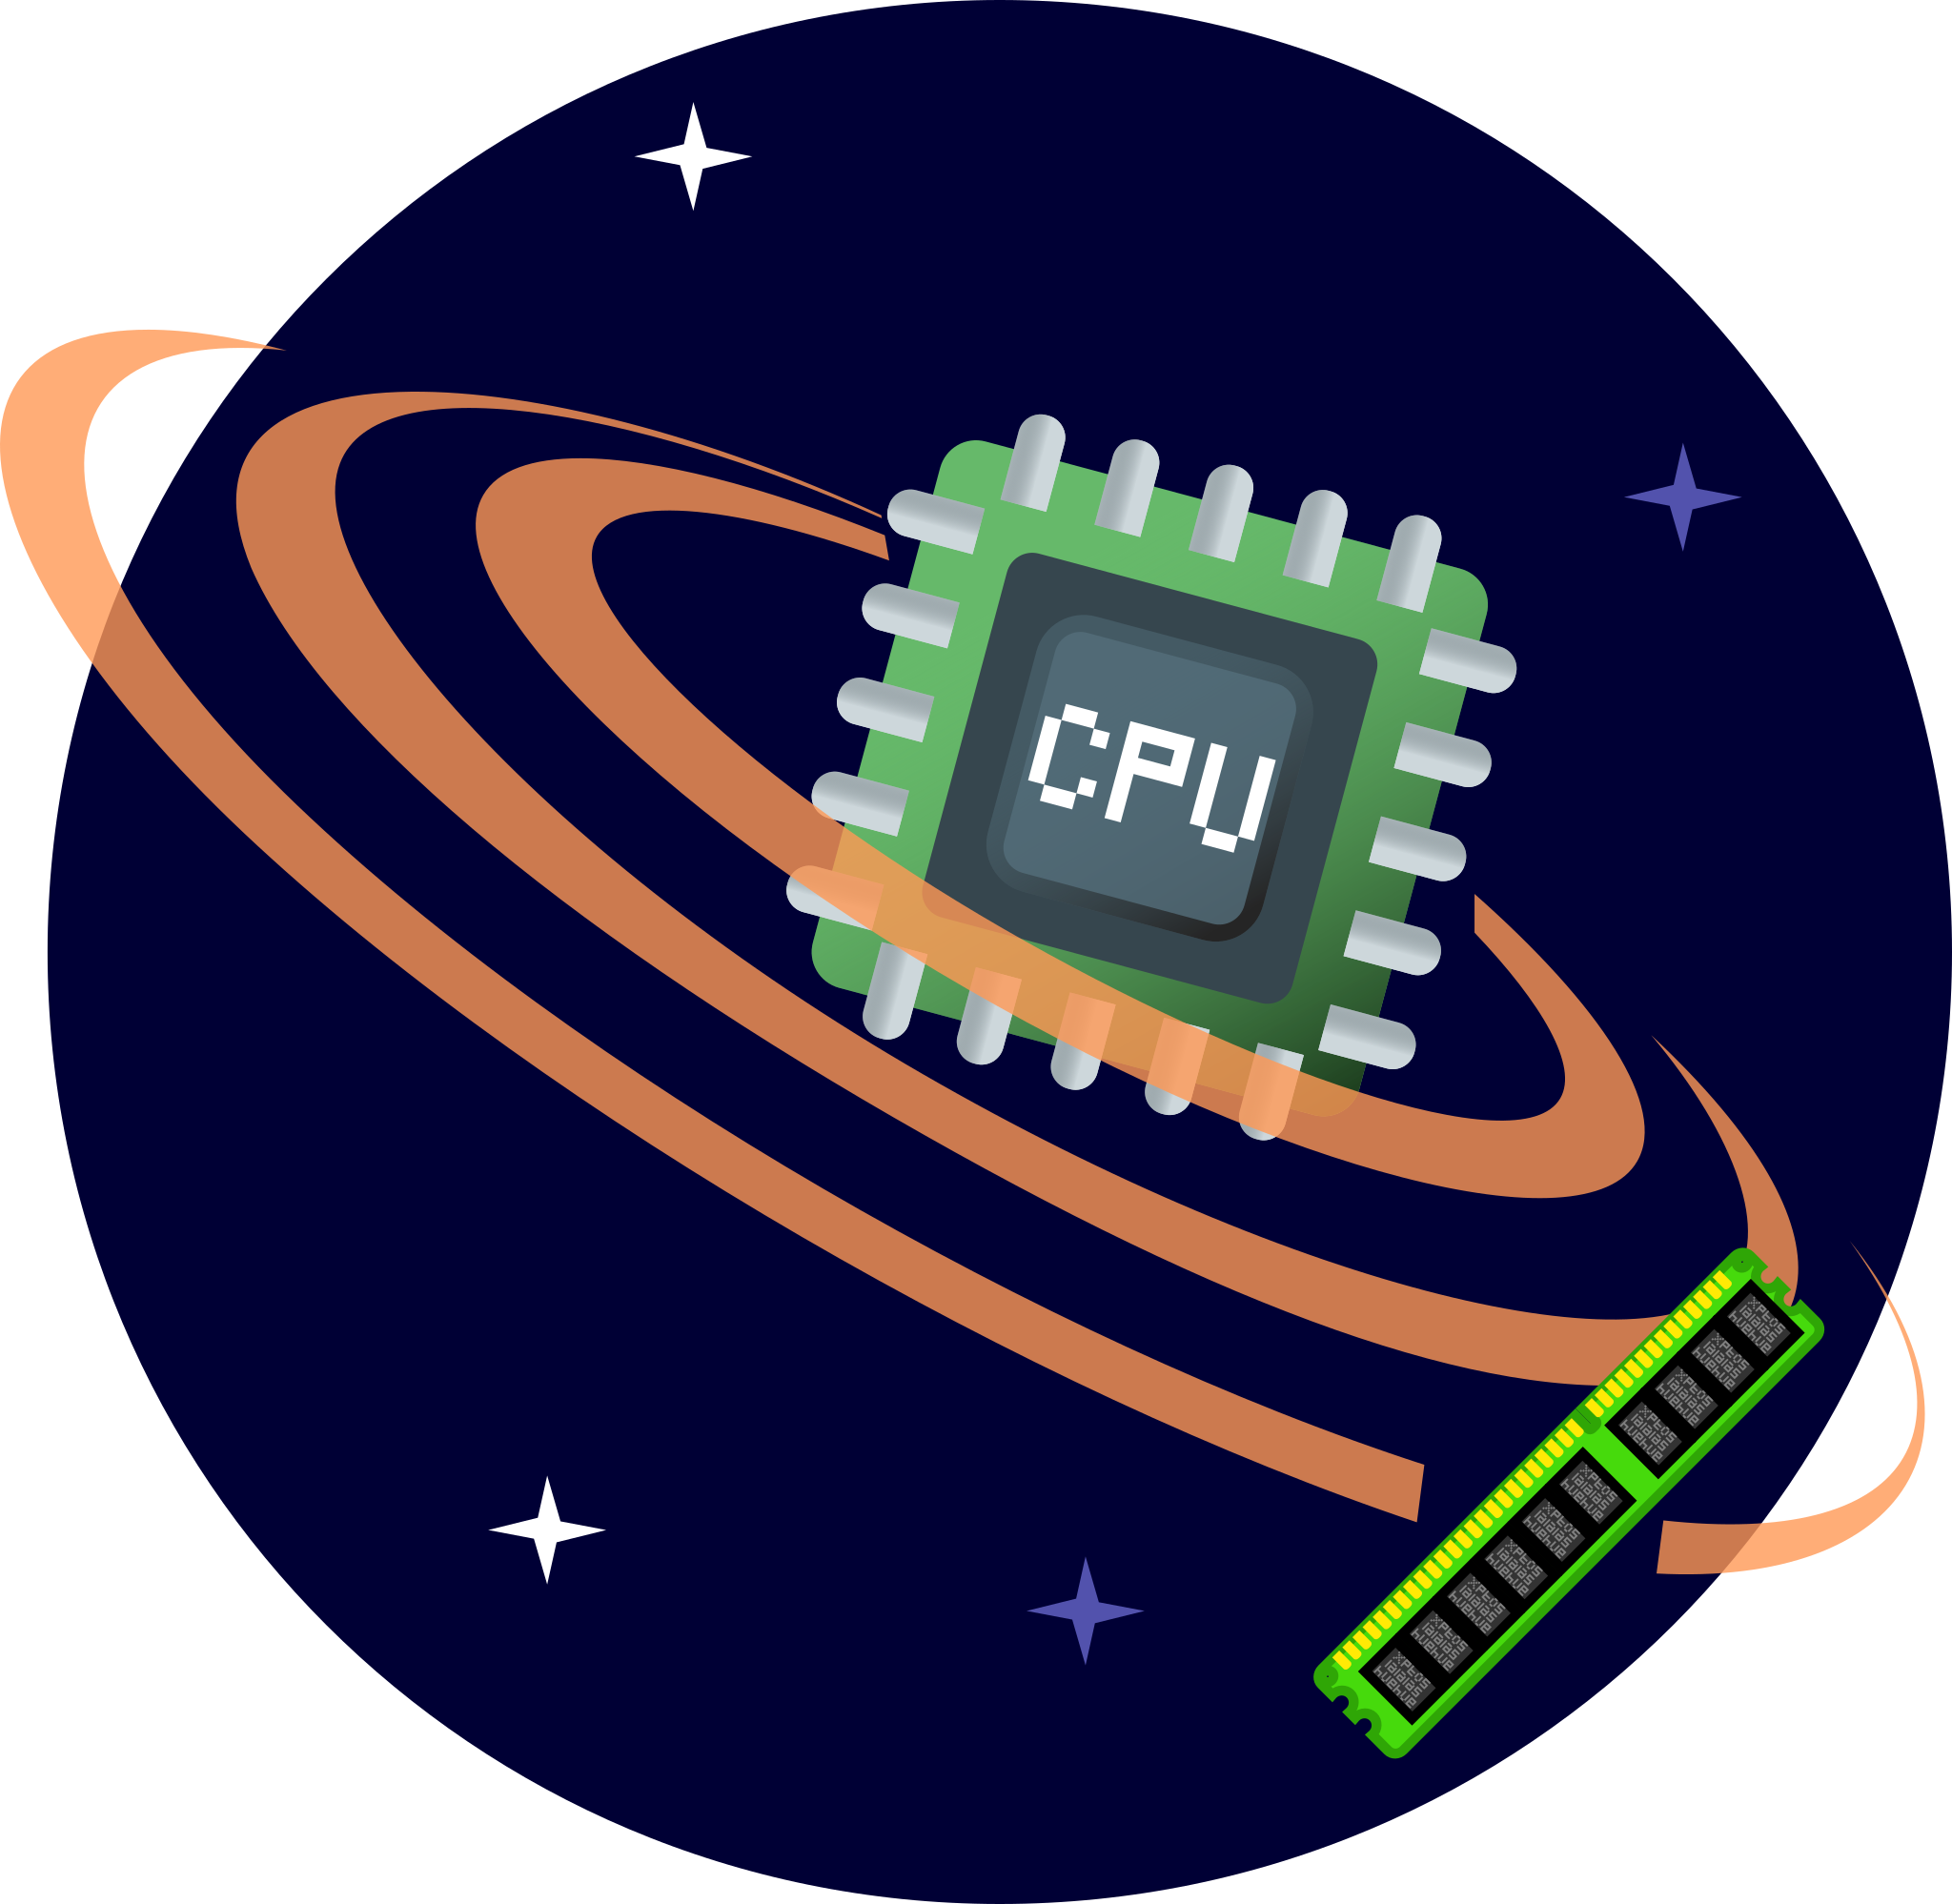
\includegraphics[width=0.7\textwidth, keepaspectratio=true]{images/cpu_centric.png}
  \end{figure}
\end{frame}

\begin{frame}{Process-centric}{Memory hierarchy}
  \begin{figure}[ht]
    \centering
    
\includegraphics[width=0.5\textwidth, keepaspectratio=true]{images/memory_hierarchy_cache.png}
  \end{figure}
\end{frame}

\begin{frame}{Process-centric}{Memory hierarchy}
  \begin{figure}[ht]
    \centering
    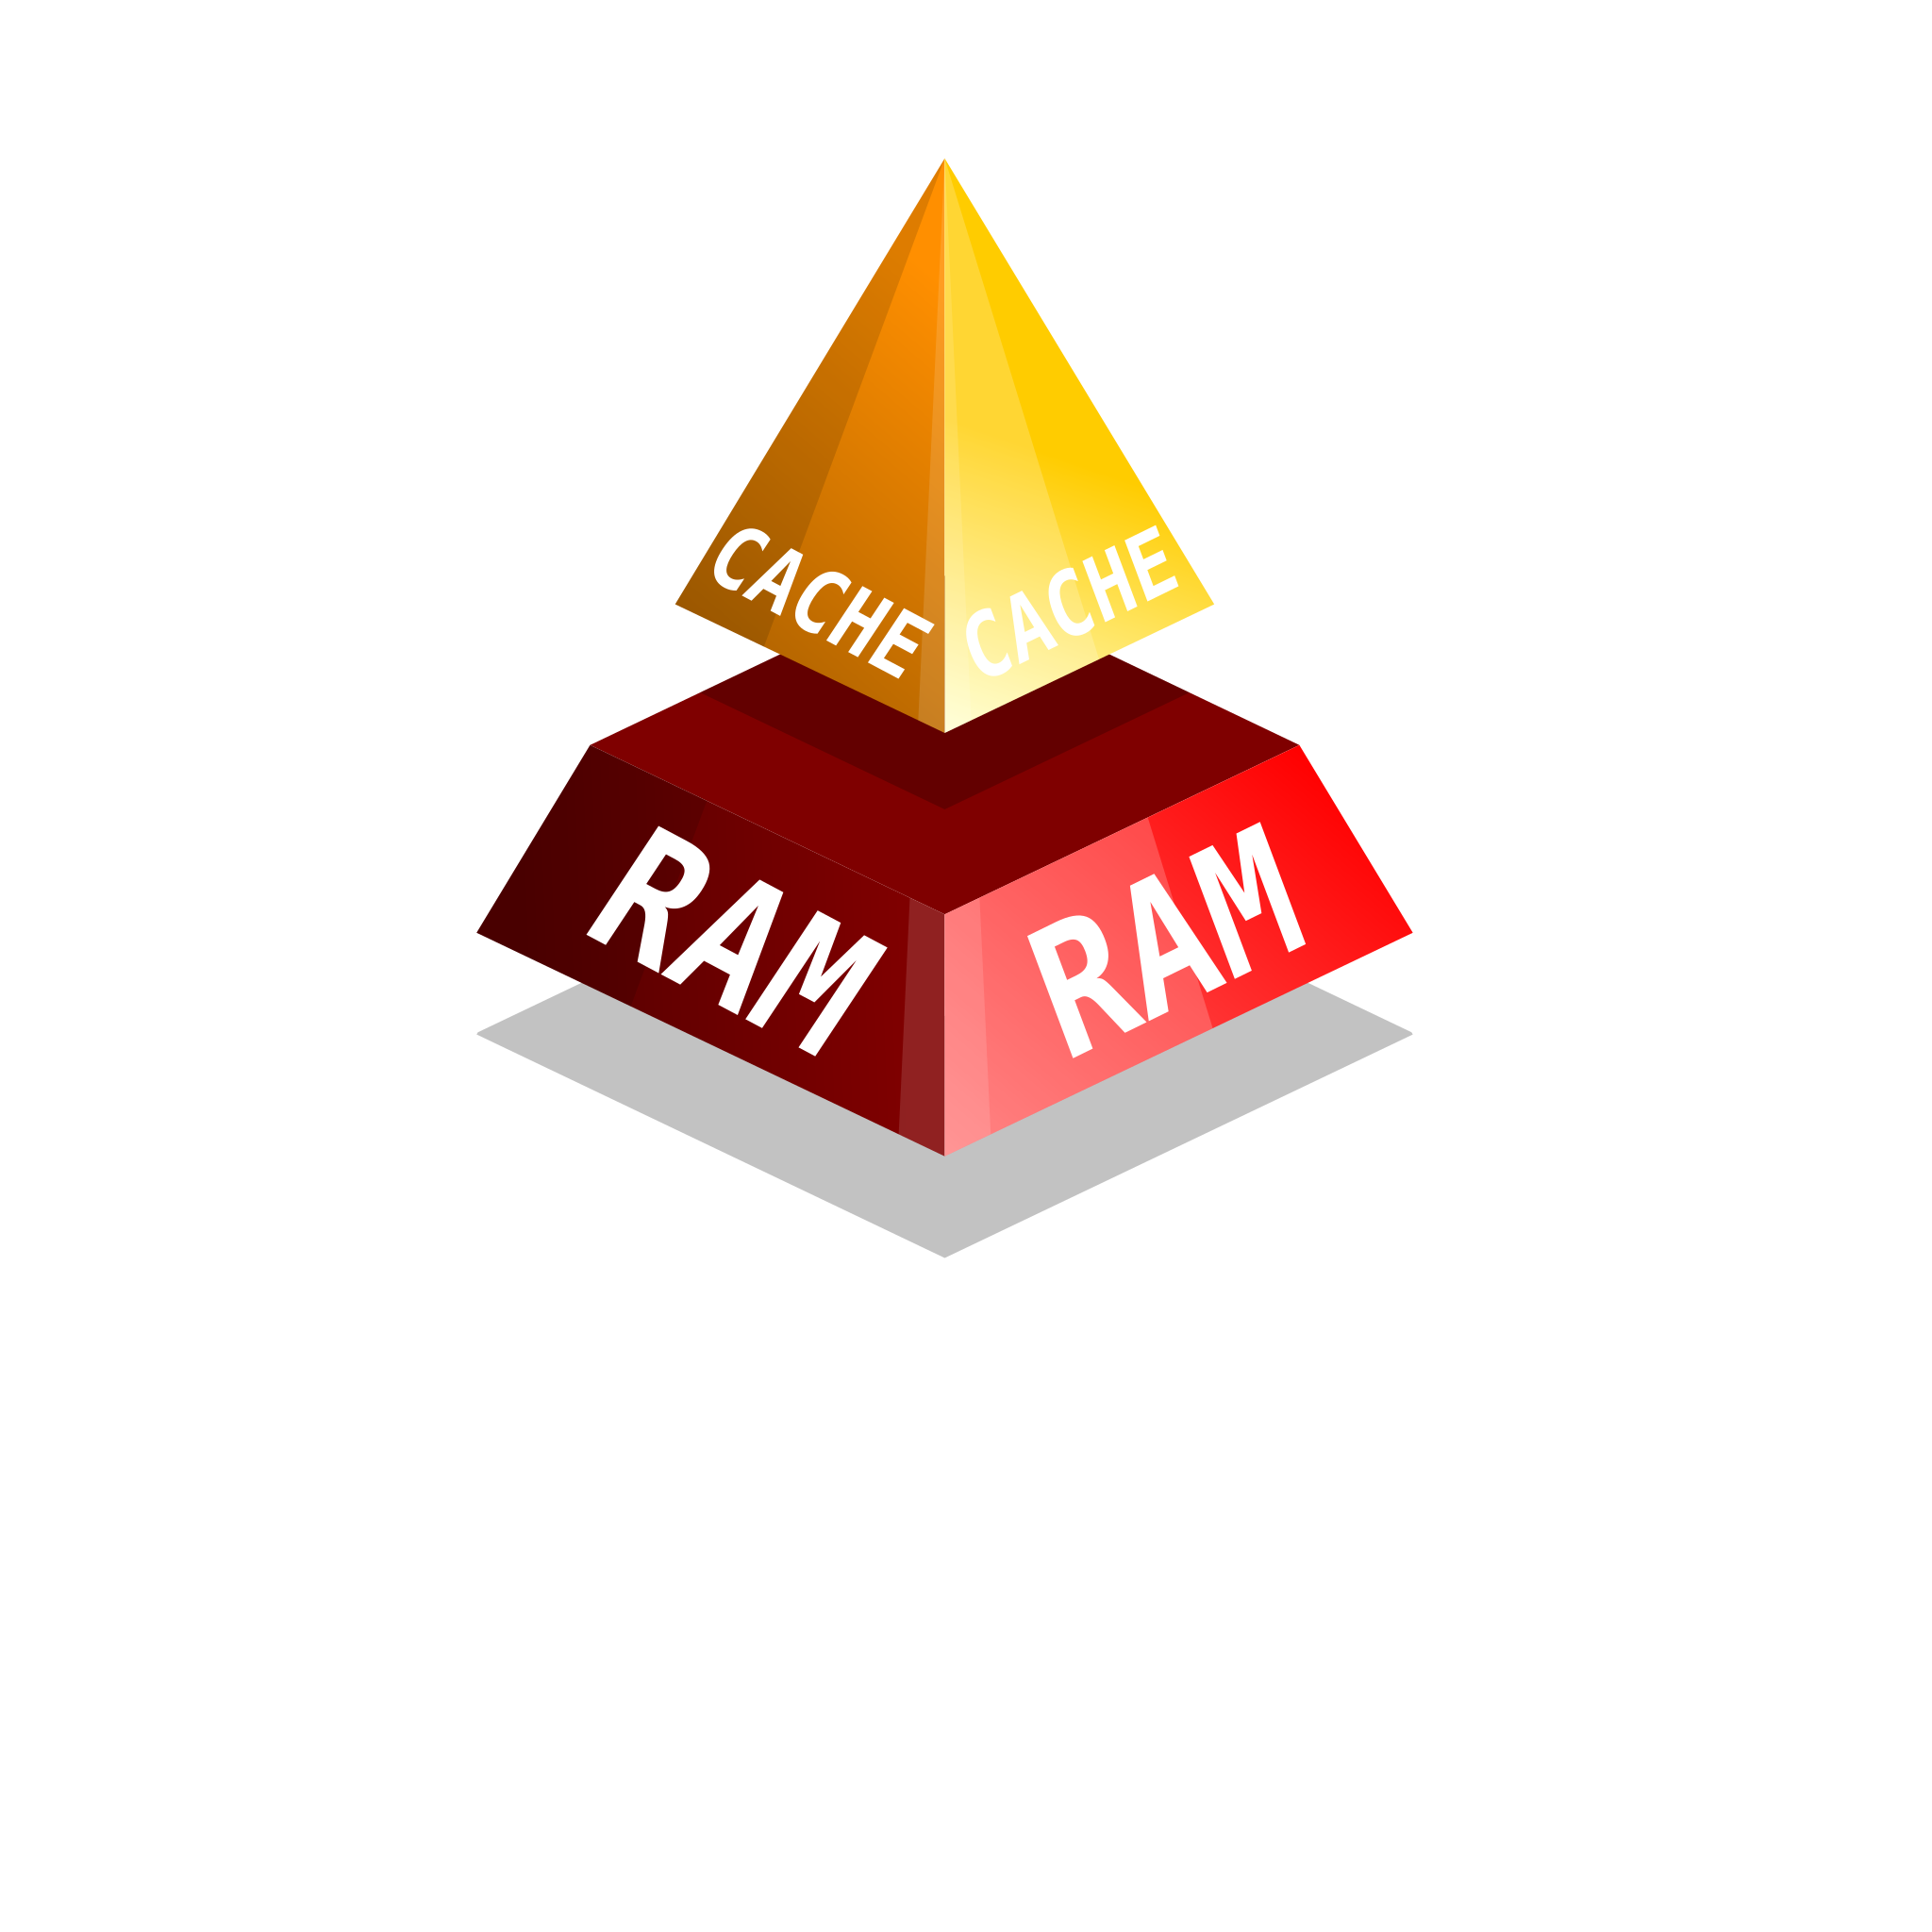
\includegraphics[width=0.5\textwidth, keepaspectratio=true]{images/memory_hierarchy_ram_cache.png}
  \end{figure}
\end{frame}

\begin{frame}{Process-centric}{Memory hierarchy}
  \begin{figure}[ht]
    \centering
    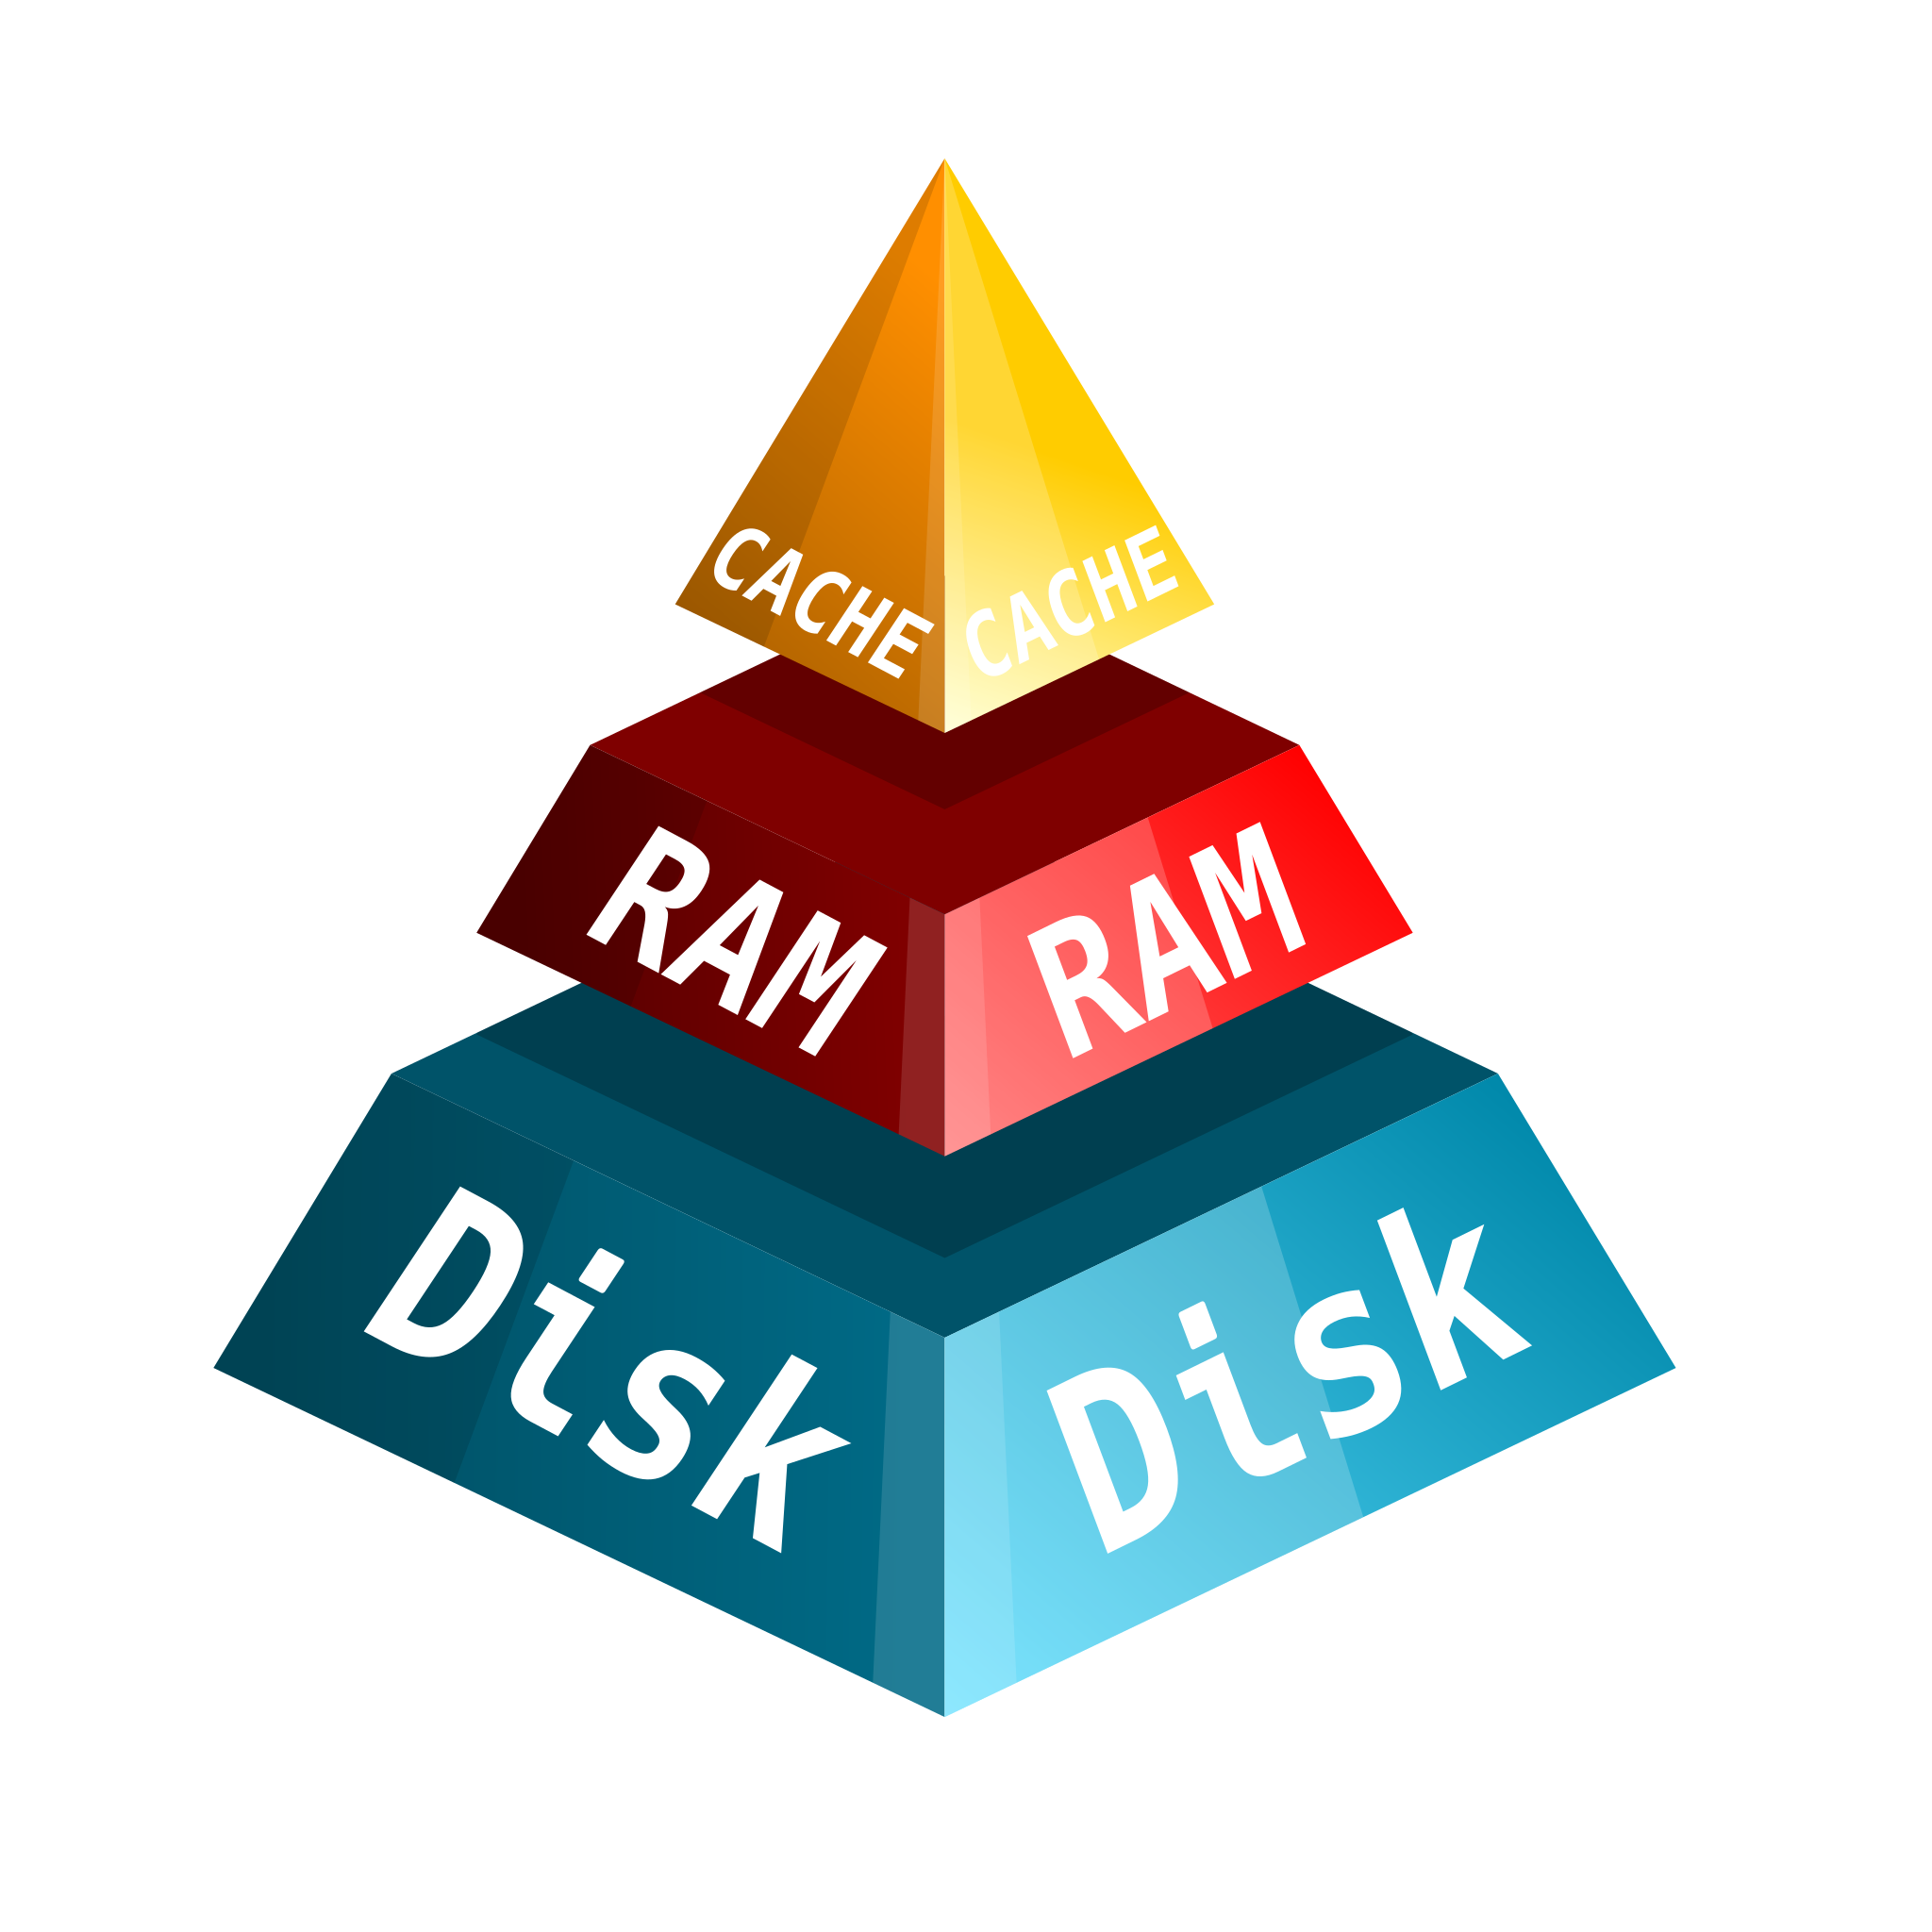
\includegraphics[width=0.5\textwidth, keepaspectratio=true]{images/memory_hierarchy_disk_ram_cache.png}
  \end{figure}
\end{frame}

%=======================================================
\section{Memory Management - Overview}
%=======================================================
\begin{frame}{Memory Management}{Overview}
  \begin{figure}[ht]
    \centering
    
\includegraphics[width=0.5\textwidth, keepaspectratio=true]{images/concepts.png}
  \end{figure}
\end{frame}


\begin{frame}{Memory Management}{Overview}
  \begin{figure}[ht]
    \centering
    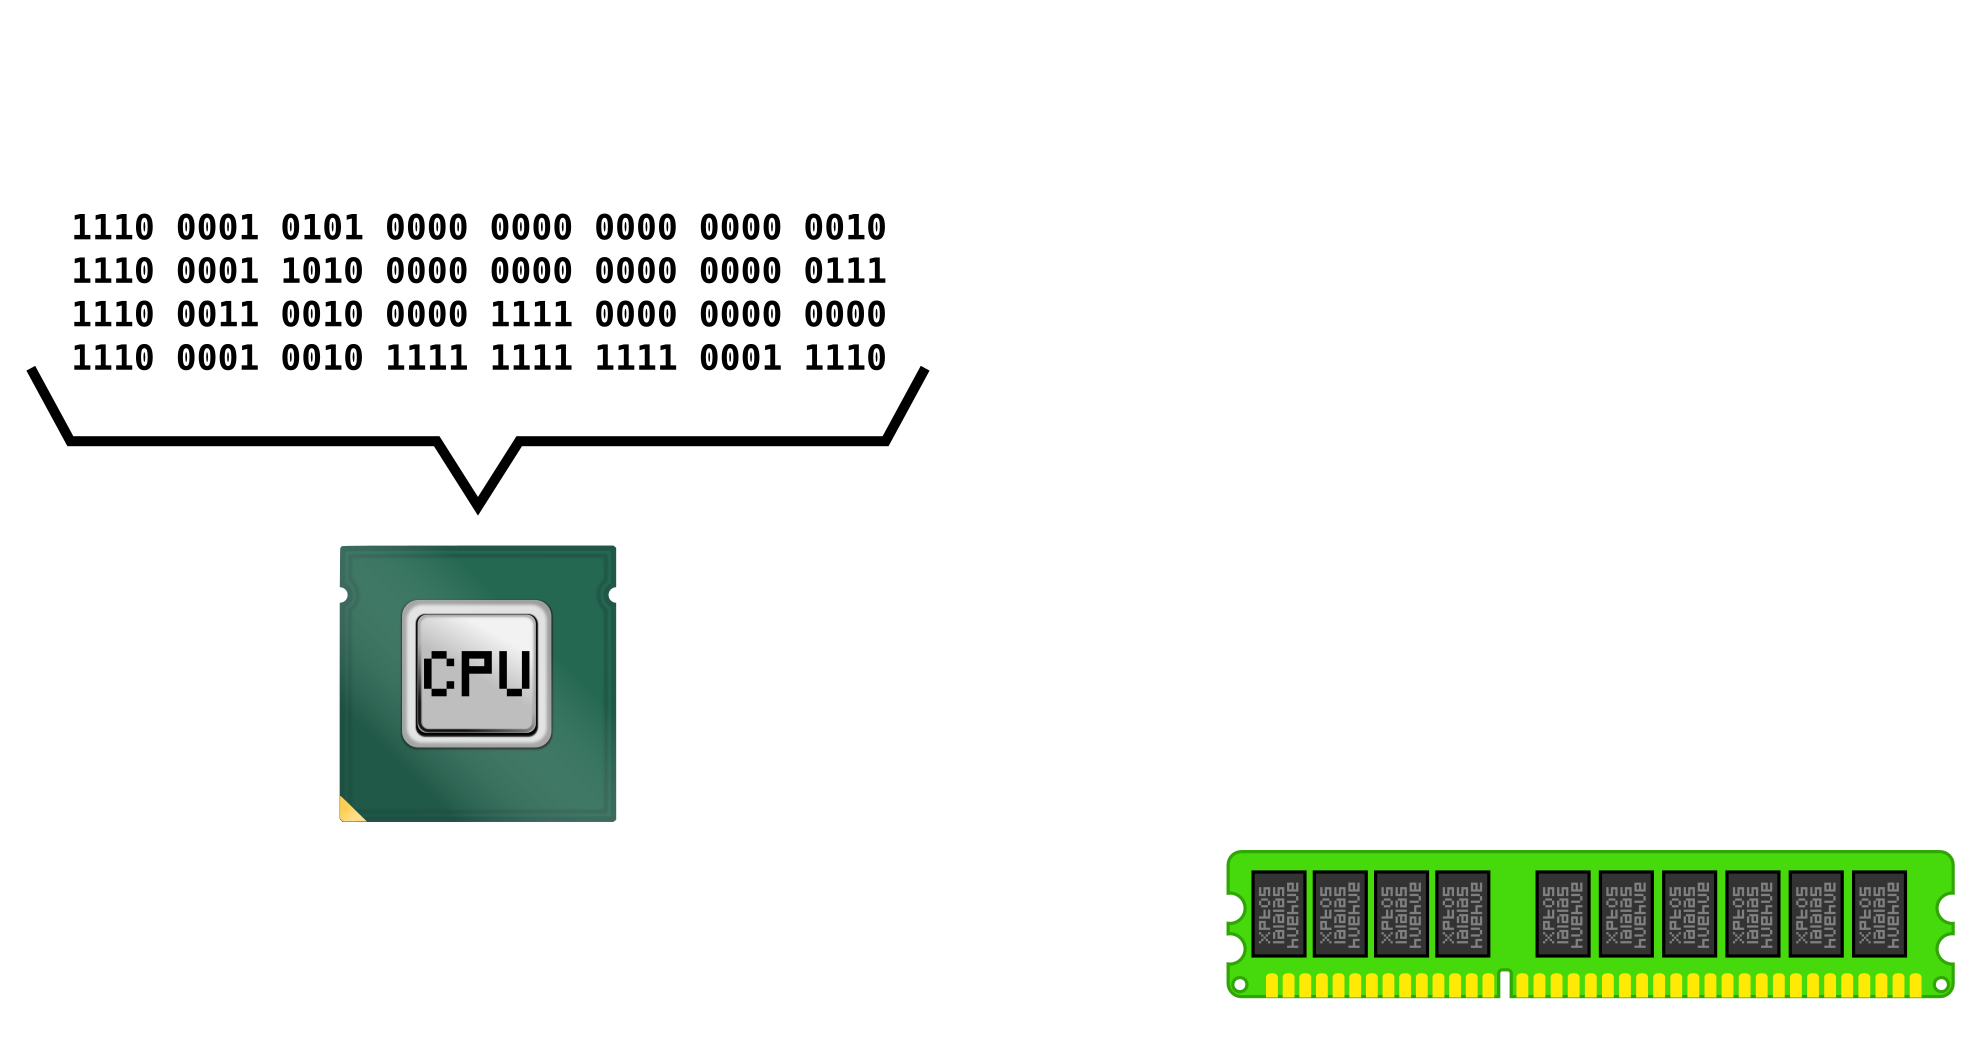
\includegraphics[width=0.9\textwidth, keepaspectratio=true]{images/virtual_memory_a.png}
  \end{figure}
\end{frame}

\begin{frame}{Memory Management}{Overview}
  \begin{figure}[ht]
    \centering
    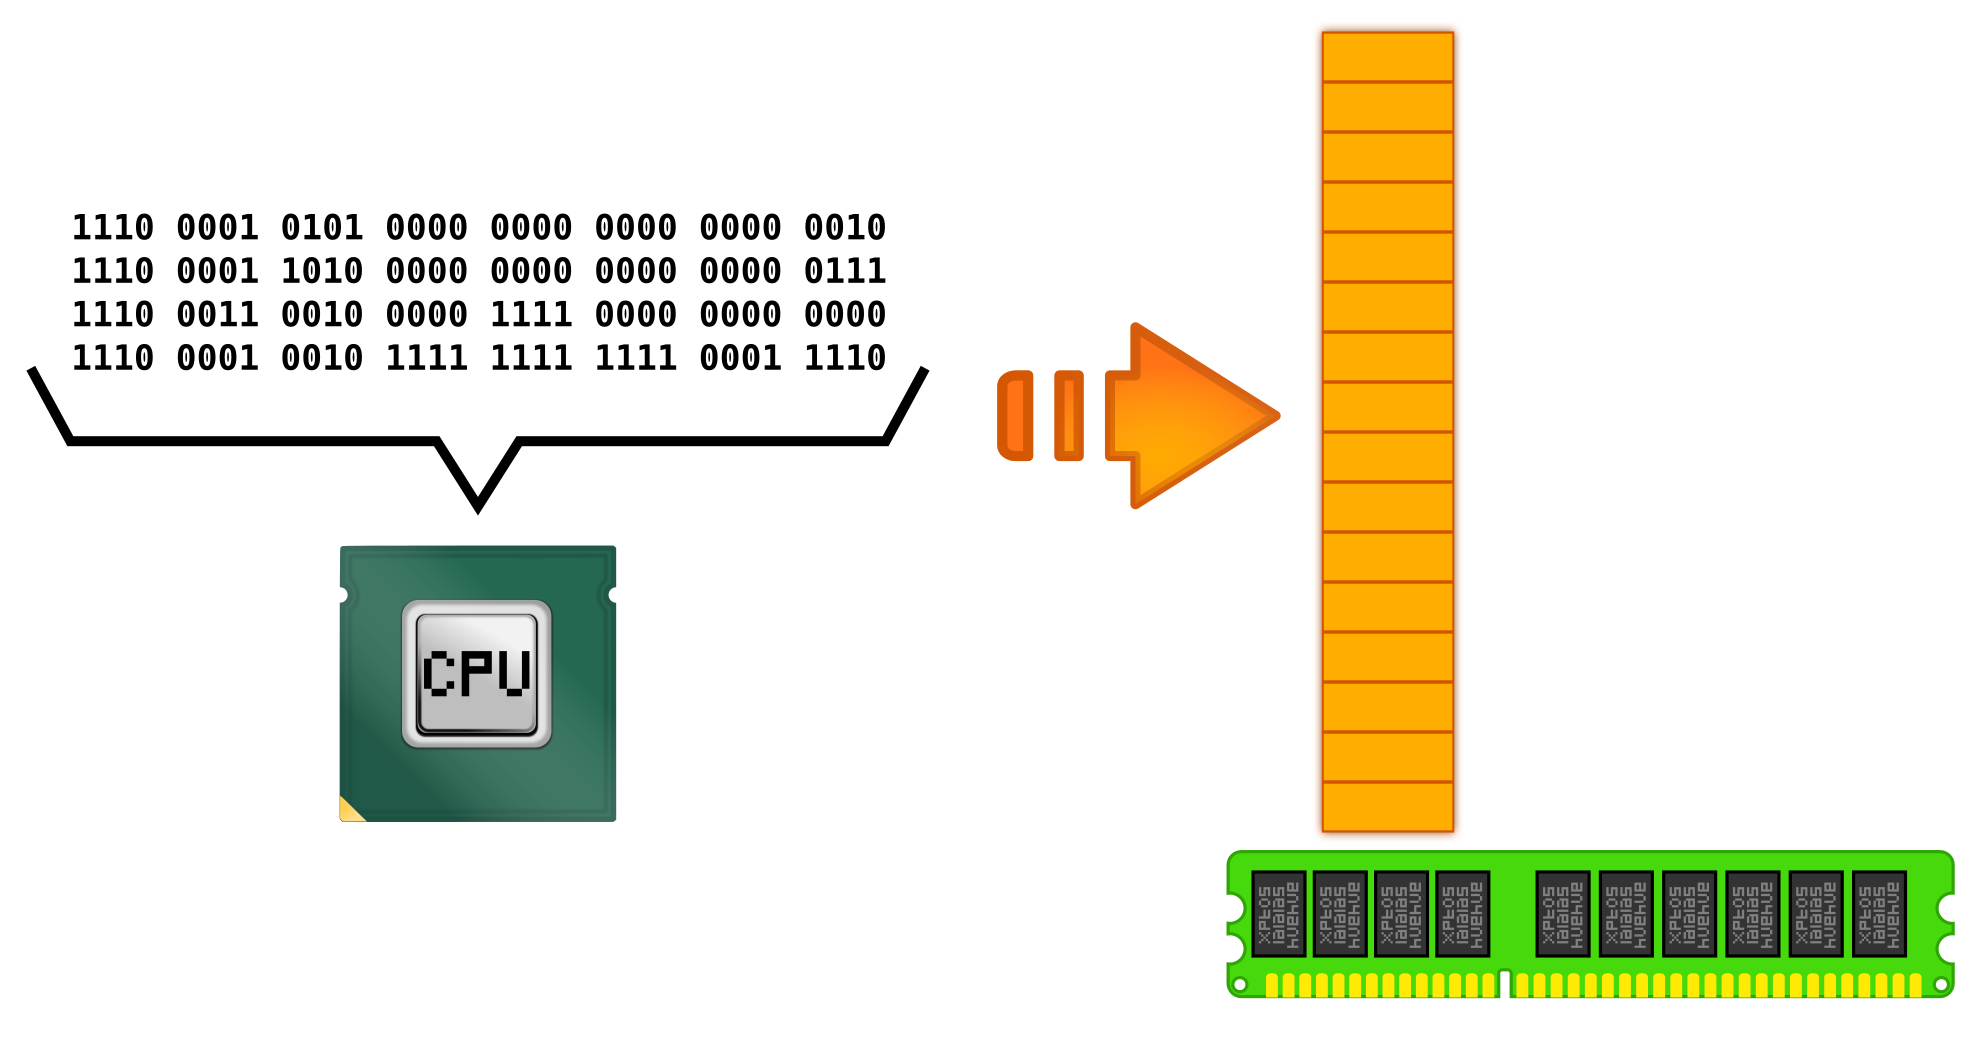
\includegraphics[width=0.9\textwidth, keepaspectratio=true]{images/virtual_memory_b.png}
  \end{figure}
\end{frame}

\begin{frame}{Memory Management}{Overview}
  \begin{figure}[ht]
    \centering
    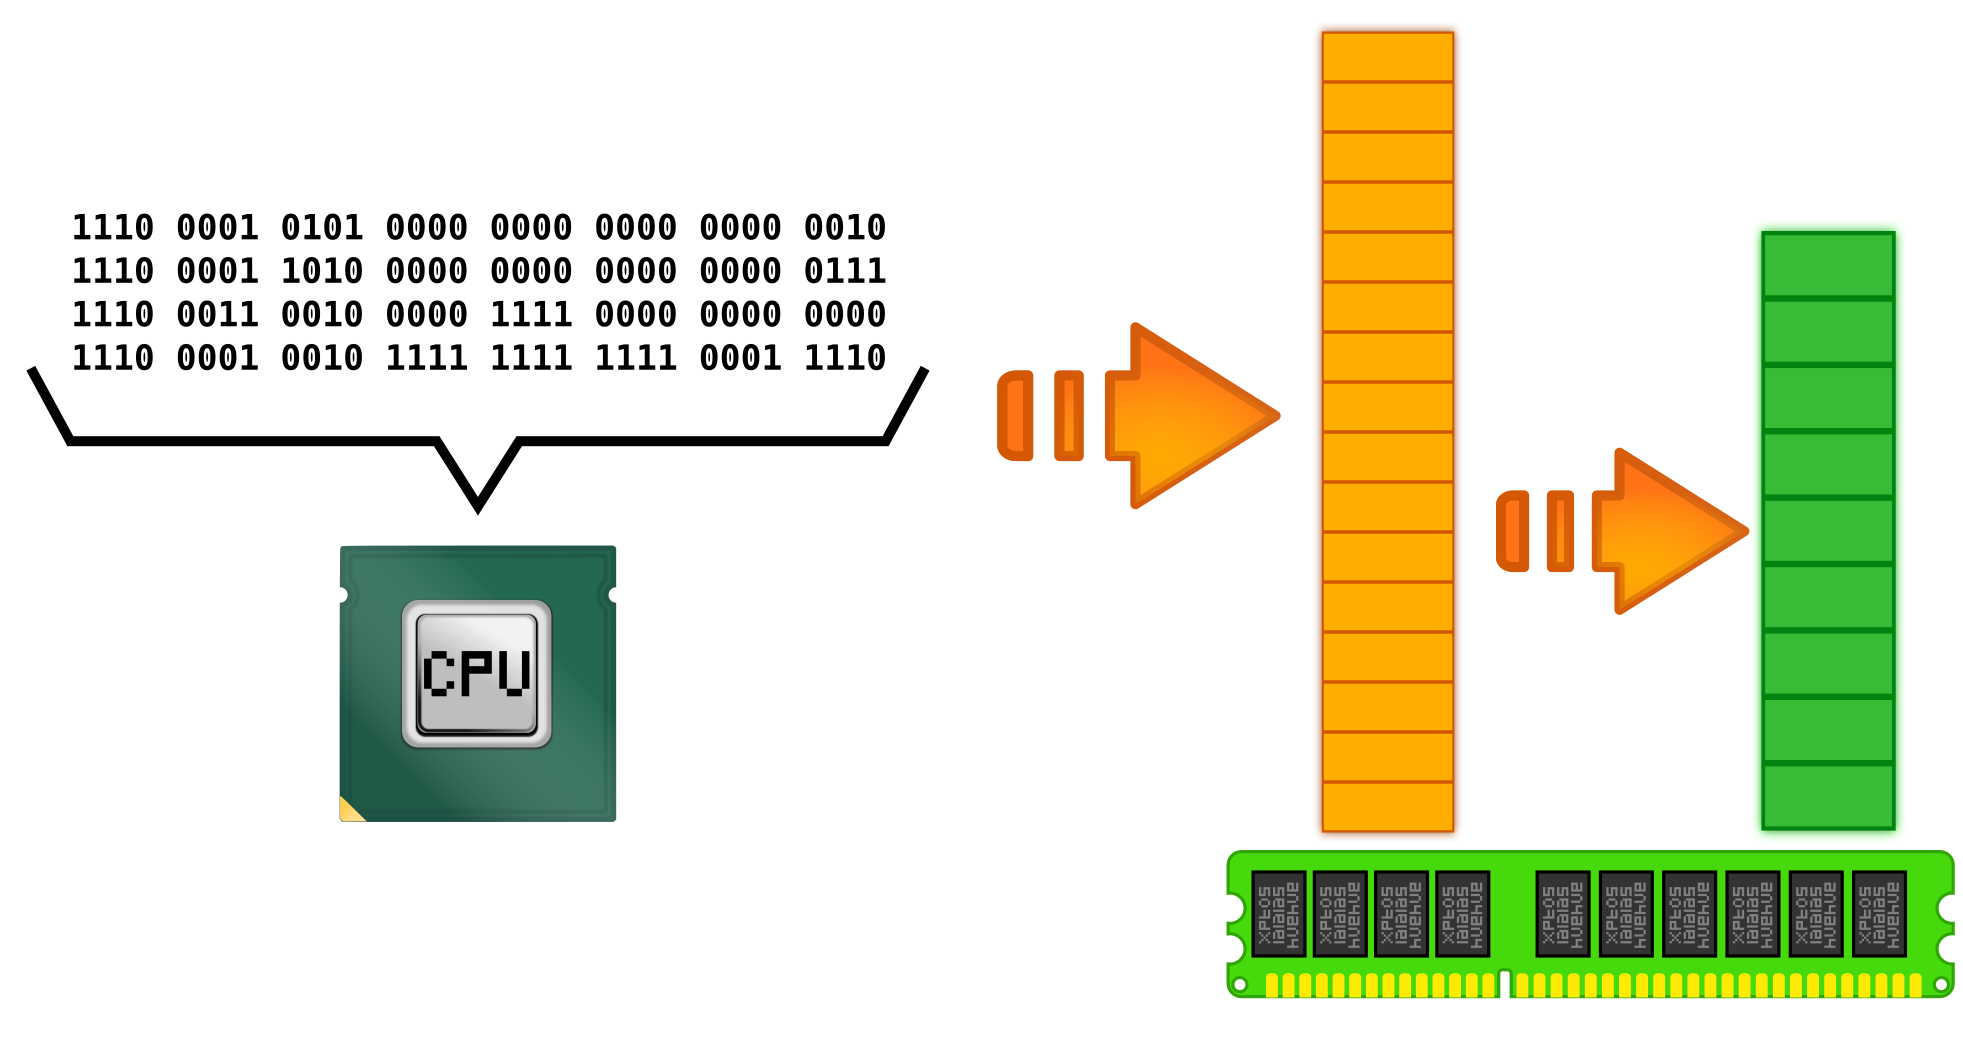
\includegraphics[width=0.9\textwidth, keepaspectratio=true]{images/virtual_memory_c.png}
  \end{figure}
\end{frame}

\begin{frame}{Memory Management}{Overview}
  \begin{figure}[ht]
    \centering
    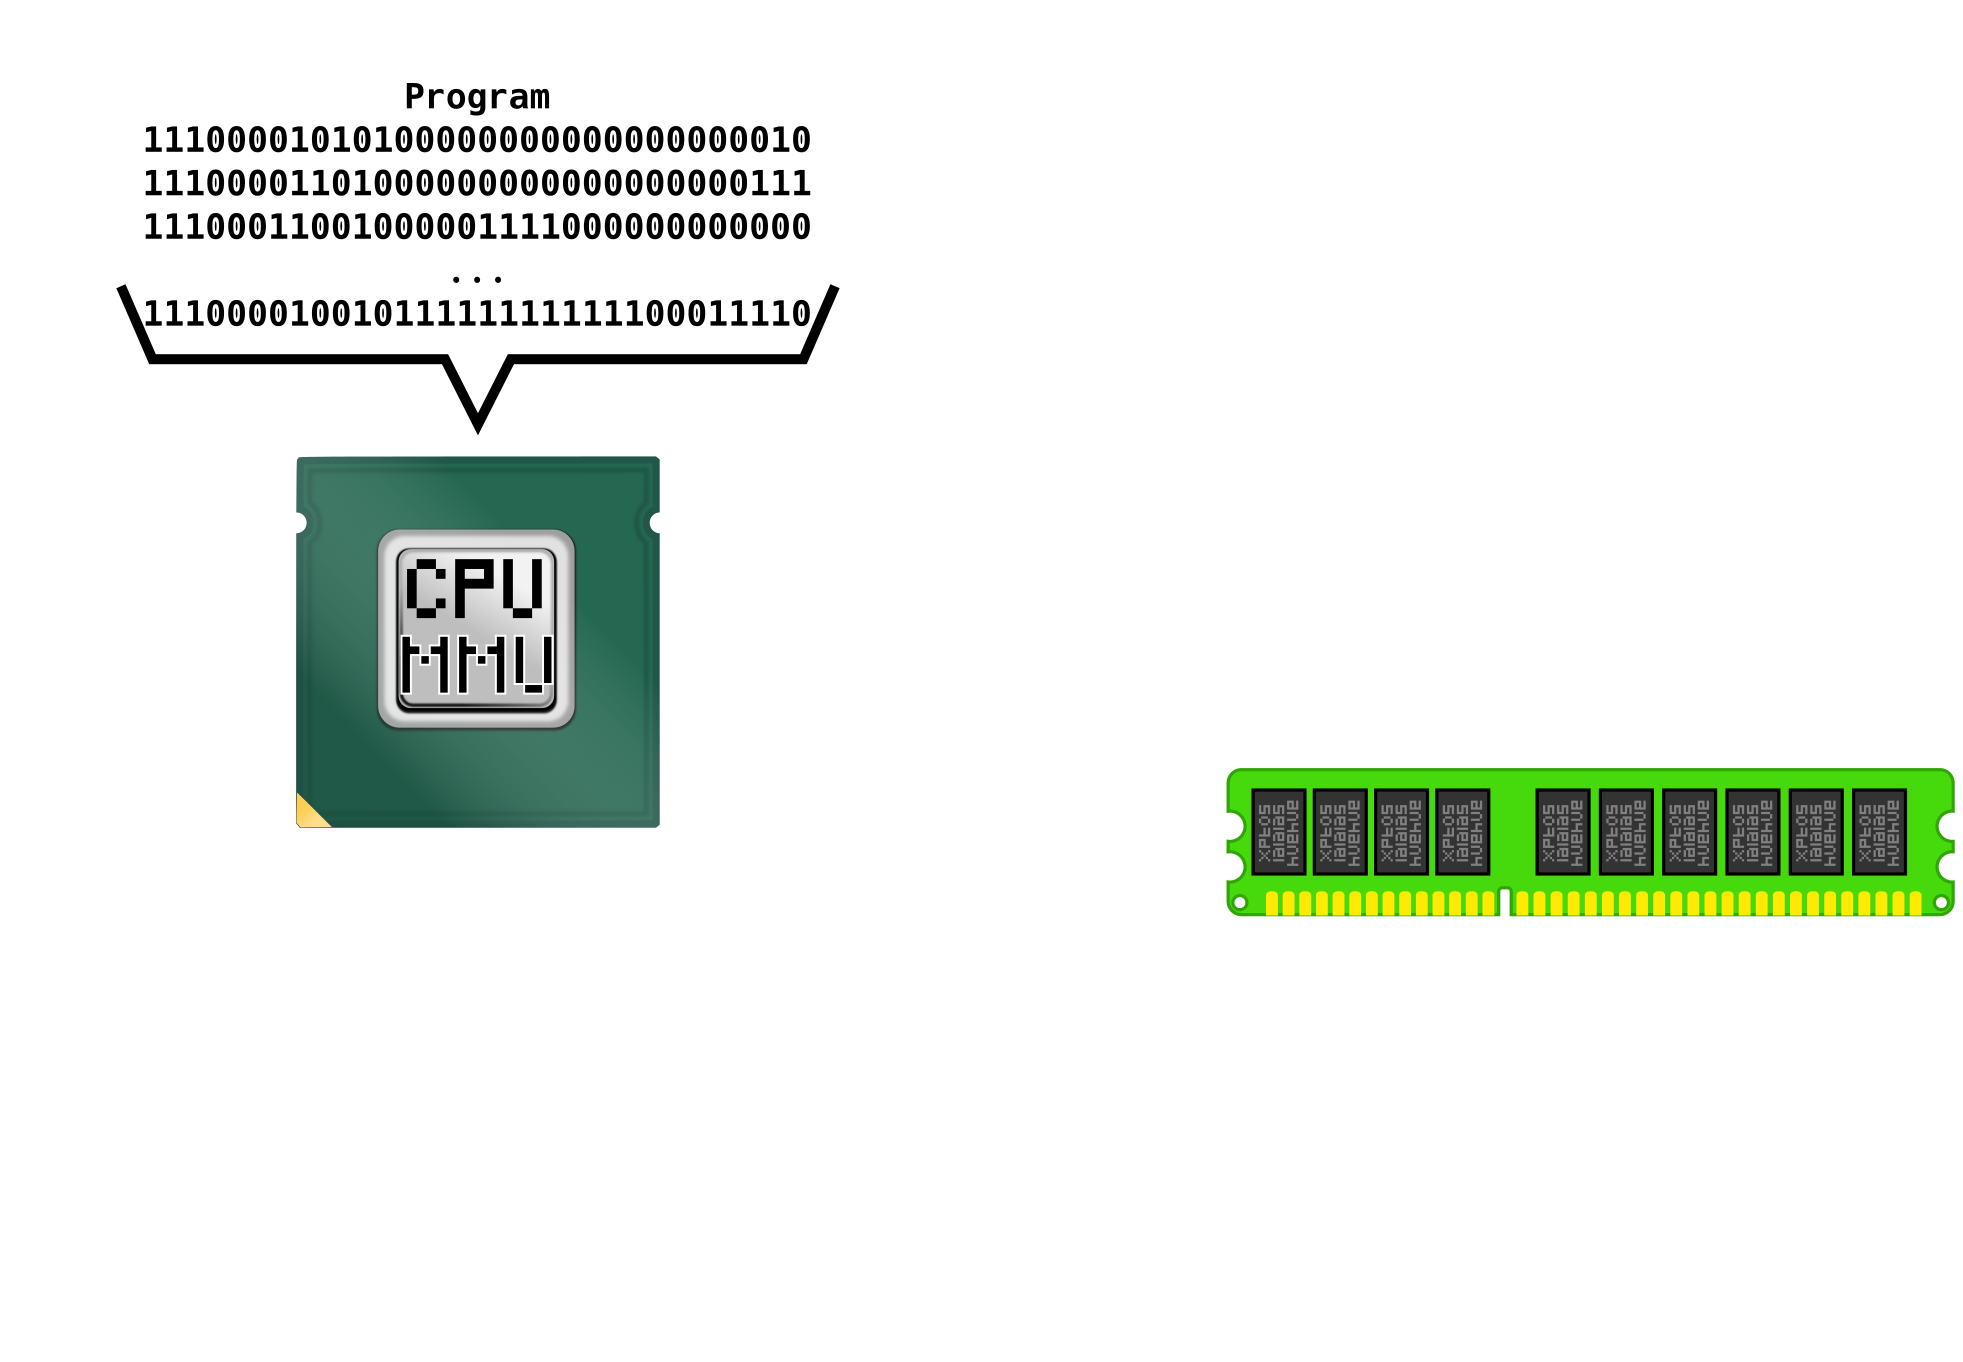
\includegraphics[width=0.9\textwidth, keepaspectratio=true]{images/mmu_a.png}
  \end{figure}
\end{frame}

\begin{frame}{Memory Management}{Overview}
  \begin{figure}[ht]
    \centering
    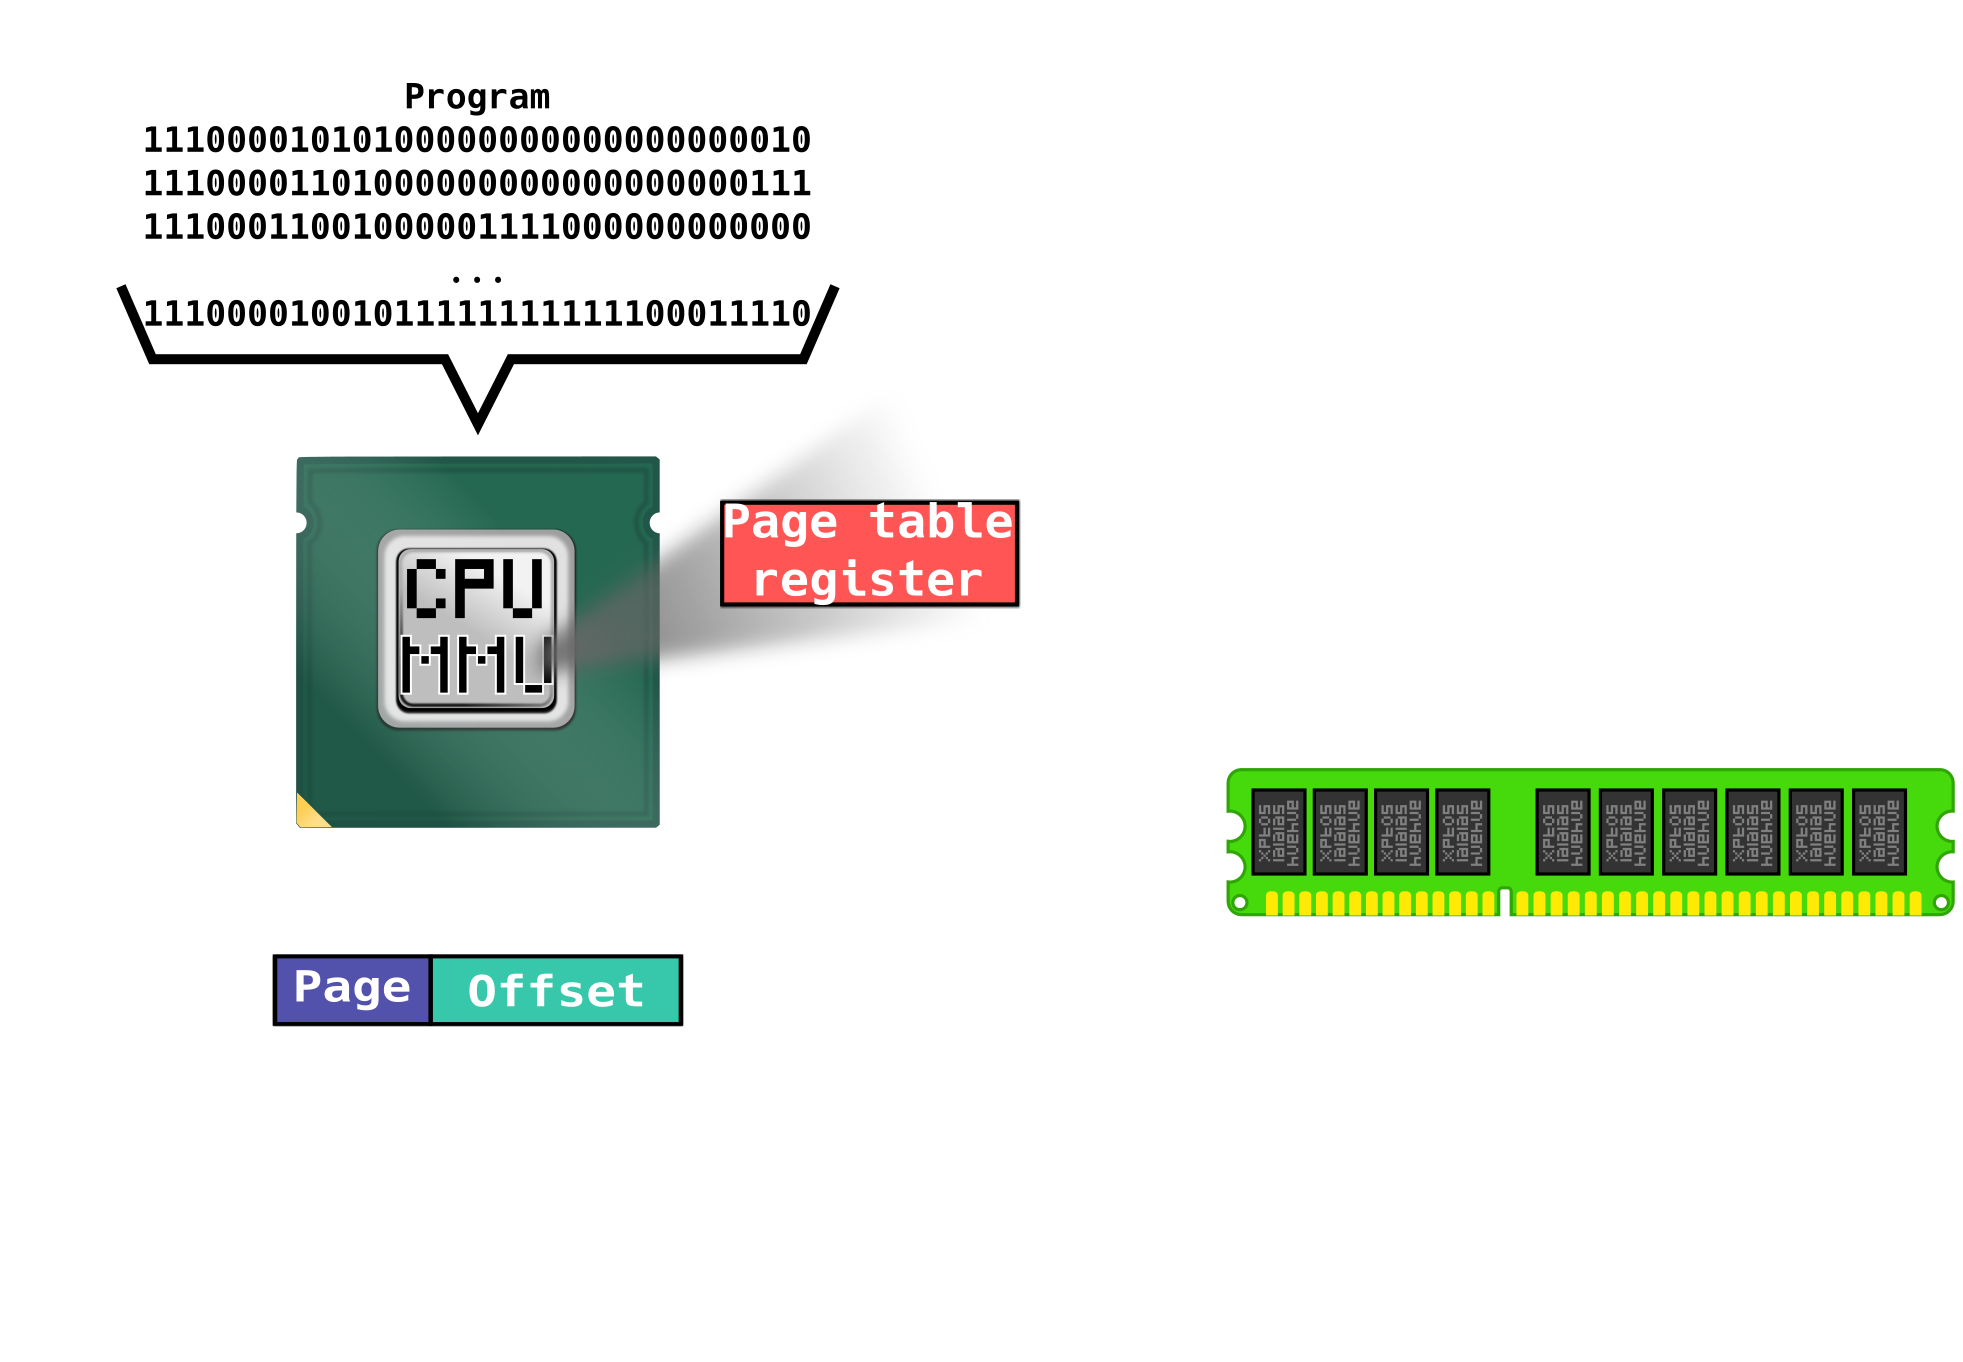
\includegraphics[width=0.9\textwidth, keepaspectratio=true]{images/mmu_b.png}
  \end{figure}
\end{frame}

\begin{frame}{Memory Management}{Overview}
  \begin{figure}[ht]
    \centering
    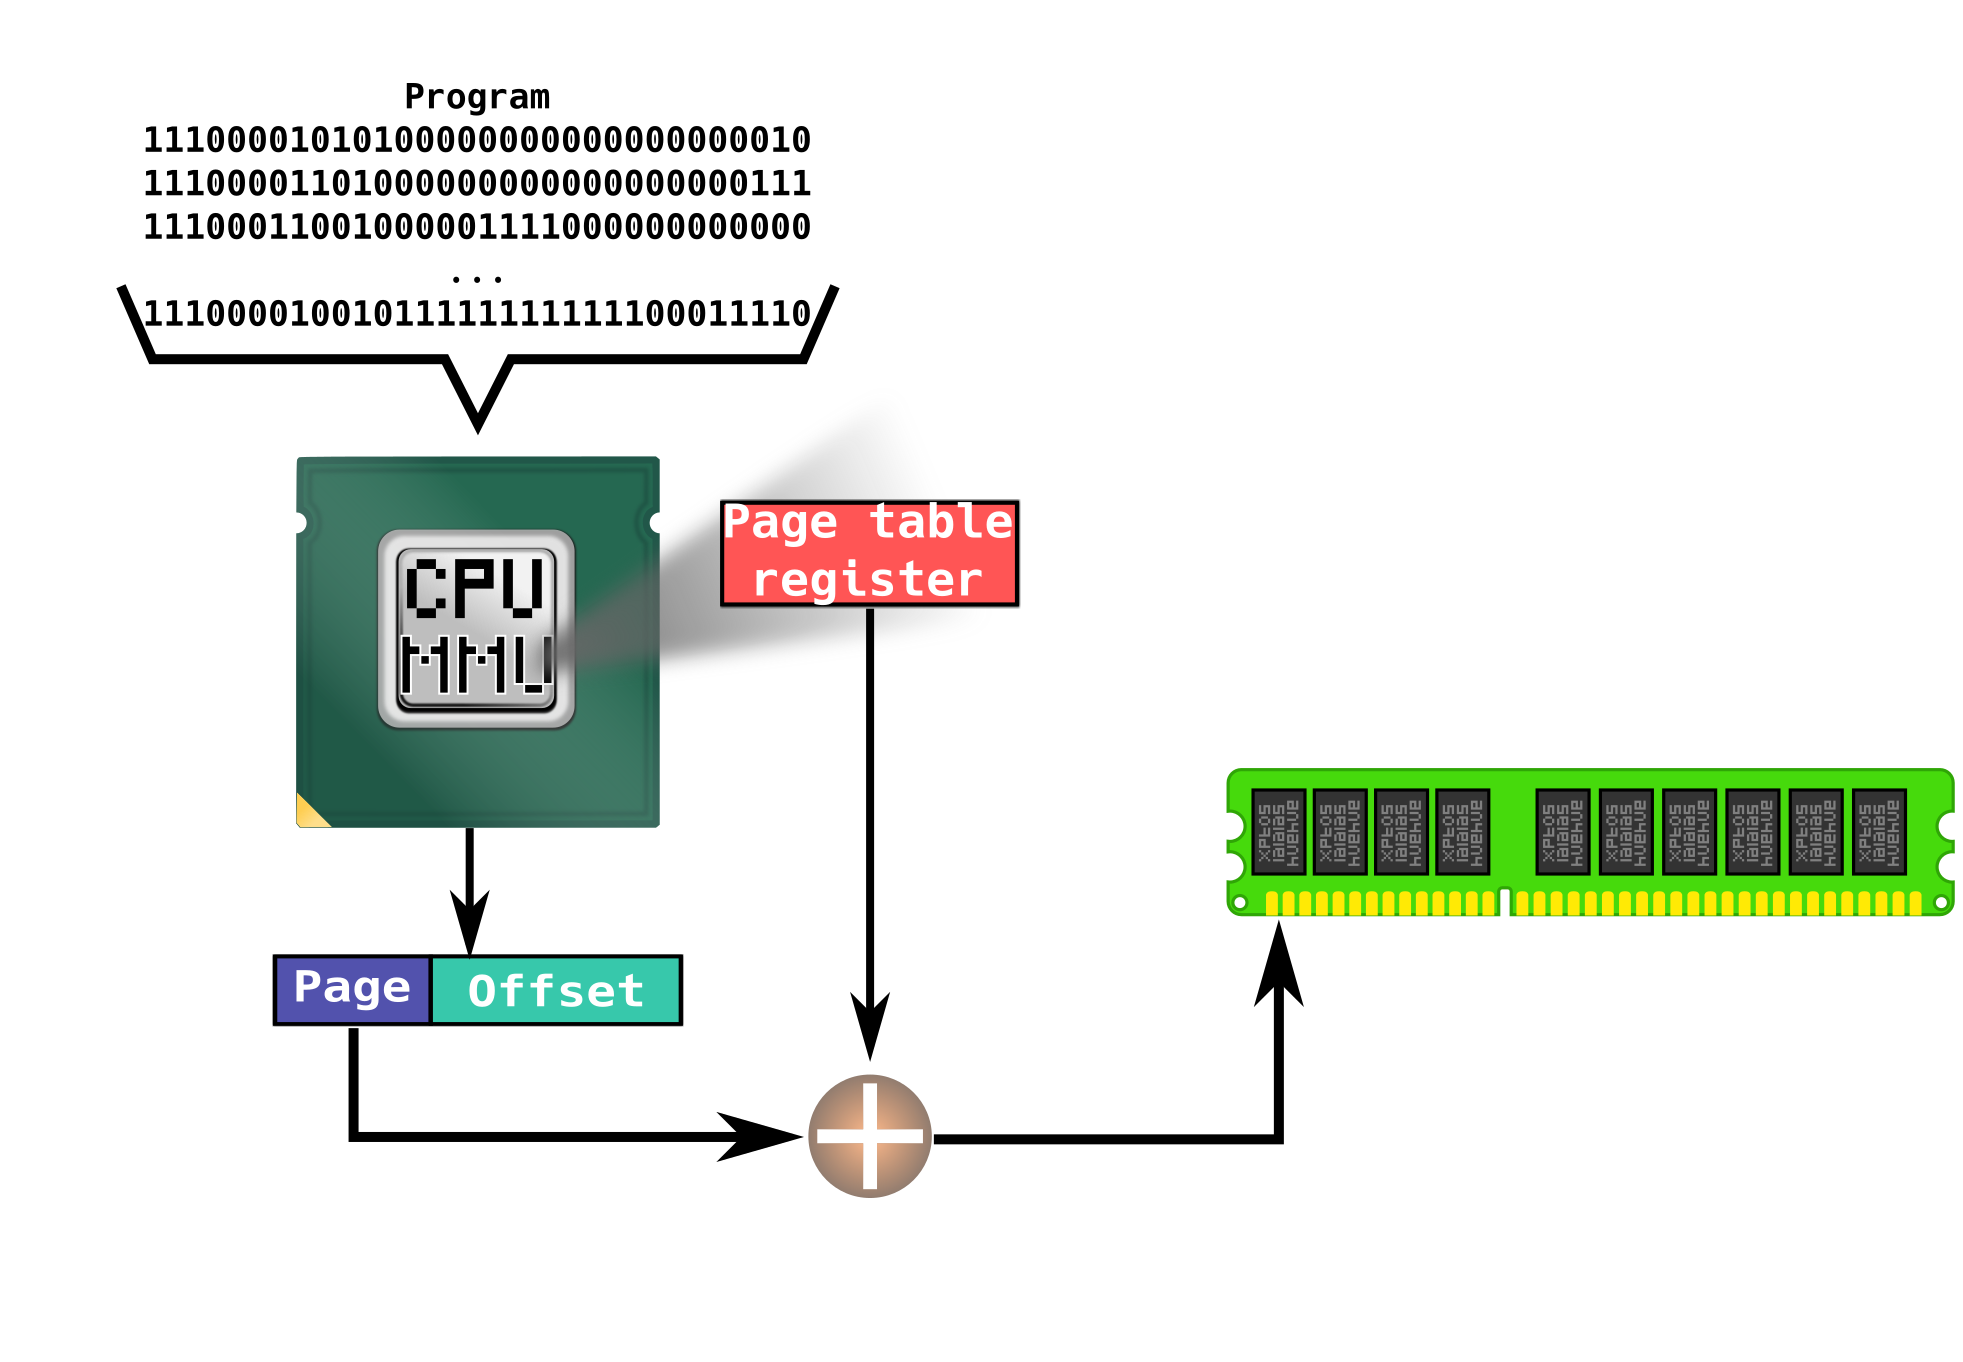
\includegraphics[width=0.9\textwidth, keepaspectratio=true]{images/mmu_c.png}
  \end{figure}
\end{frame}

\begin{frame}{Memory Management}{Overview}
  \begin{figure}[ht]
    \centering
    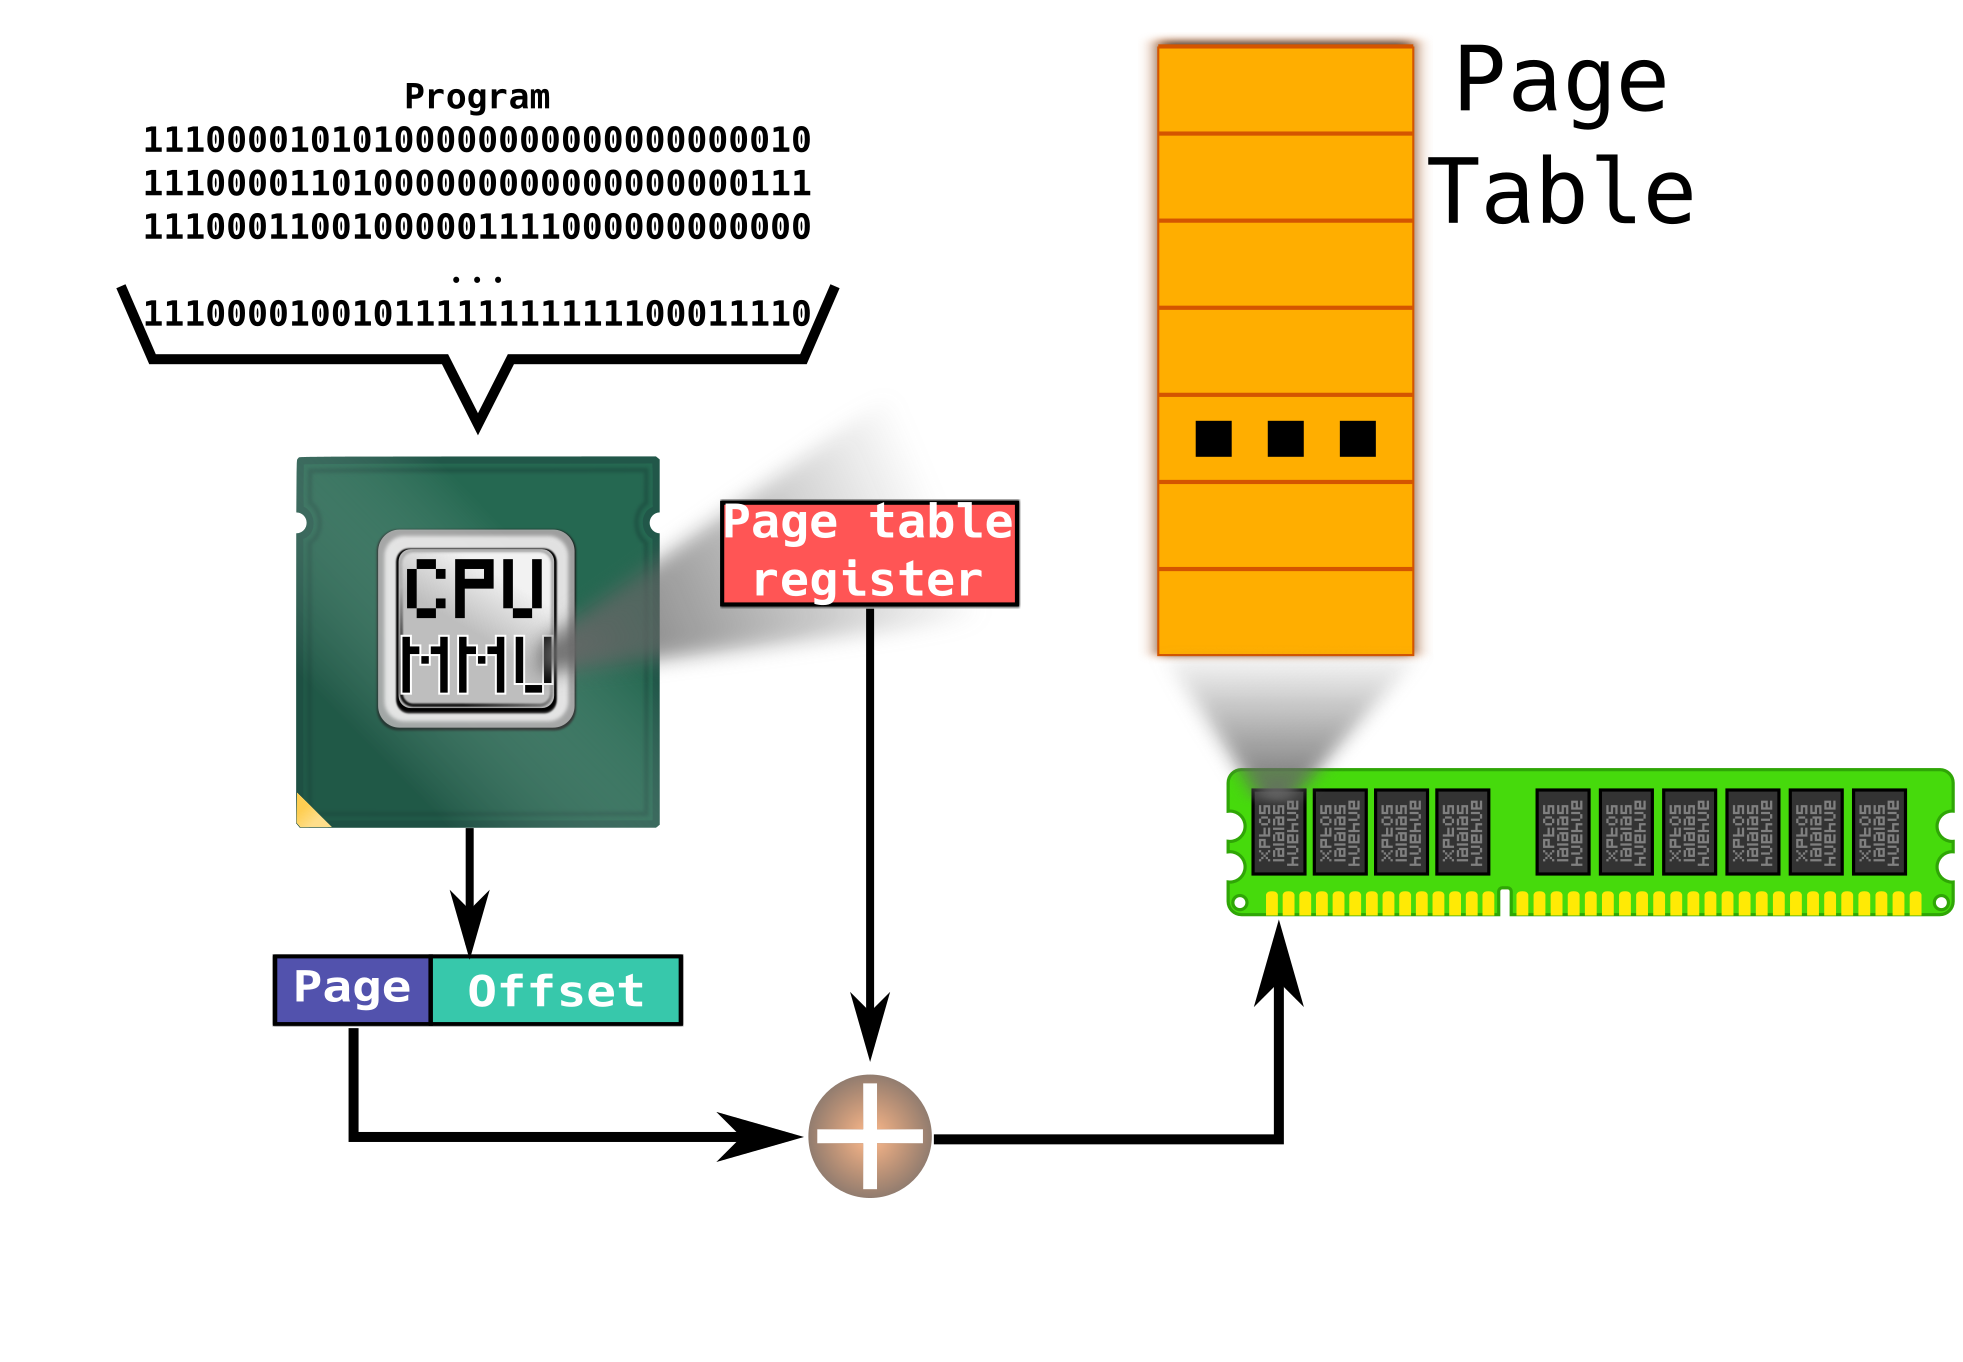
\includegraphics[width=0.9\textwidth, keepaspectratio=true]{images/mmu_d.png}
  \end{figure}
\end{frame}

\begin{frame}{Memory Management}{Overview}
  \begin{figure}[ht]
    \centering
    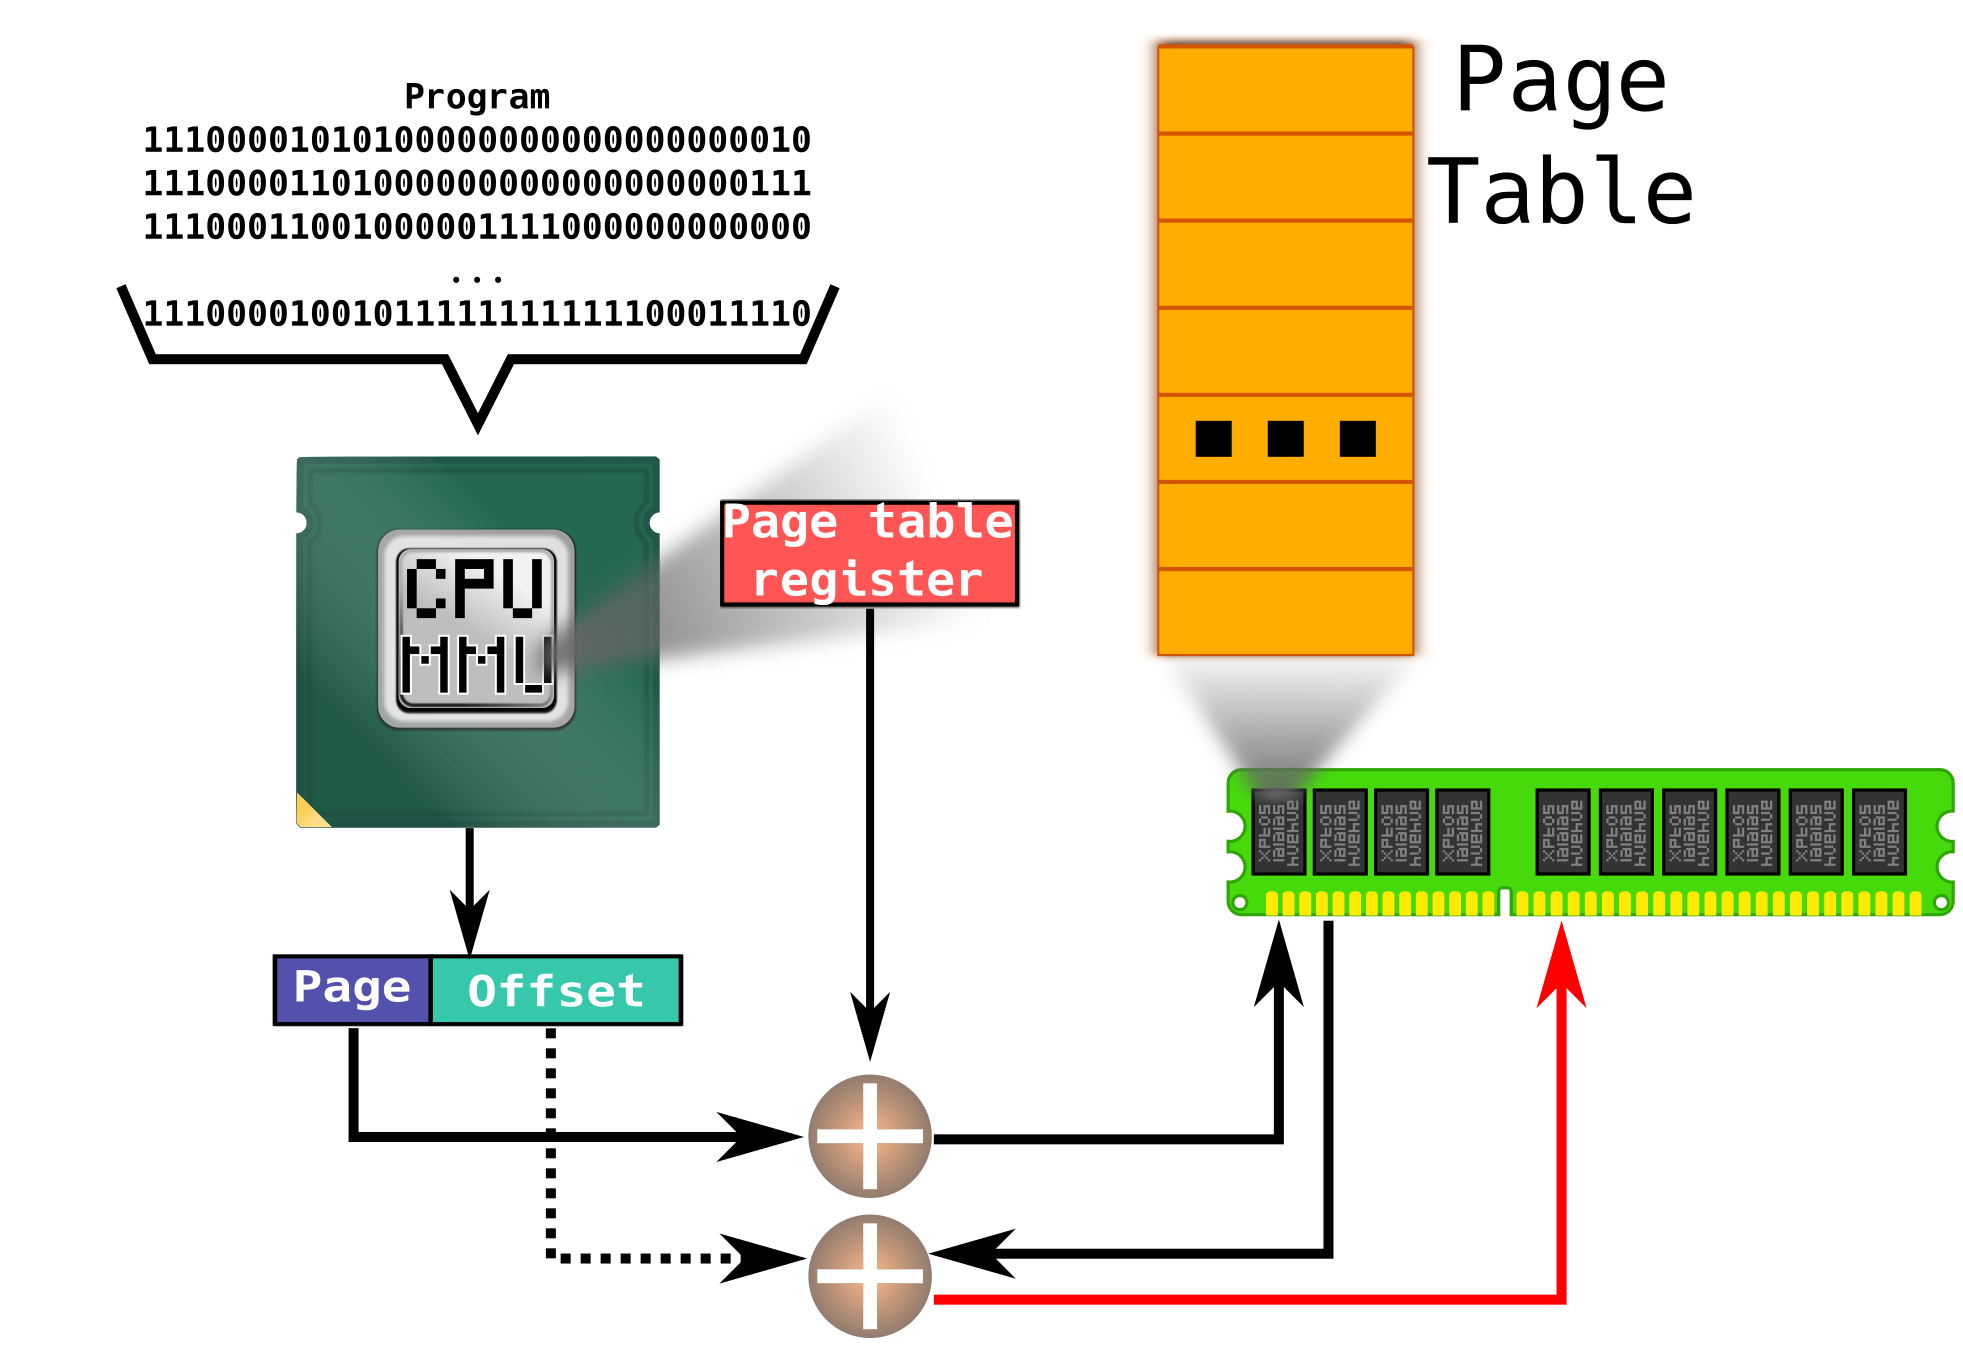
\includegraphics[width=0.9\textwidth, keepaspectratio=true]{images/mmu_e.png}
  \end{figure}
\end{frame}

\begin{frame}{Memory Management}{Overview}
  \begin{figure}[ht]
    \centering
    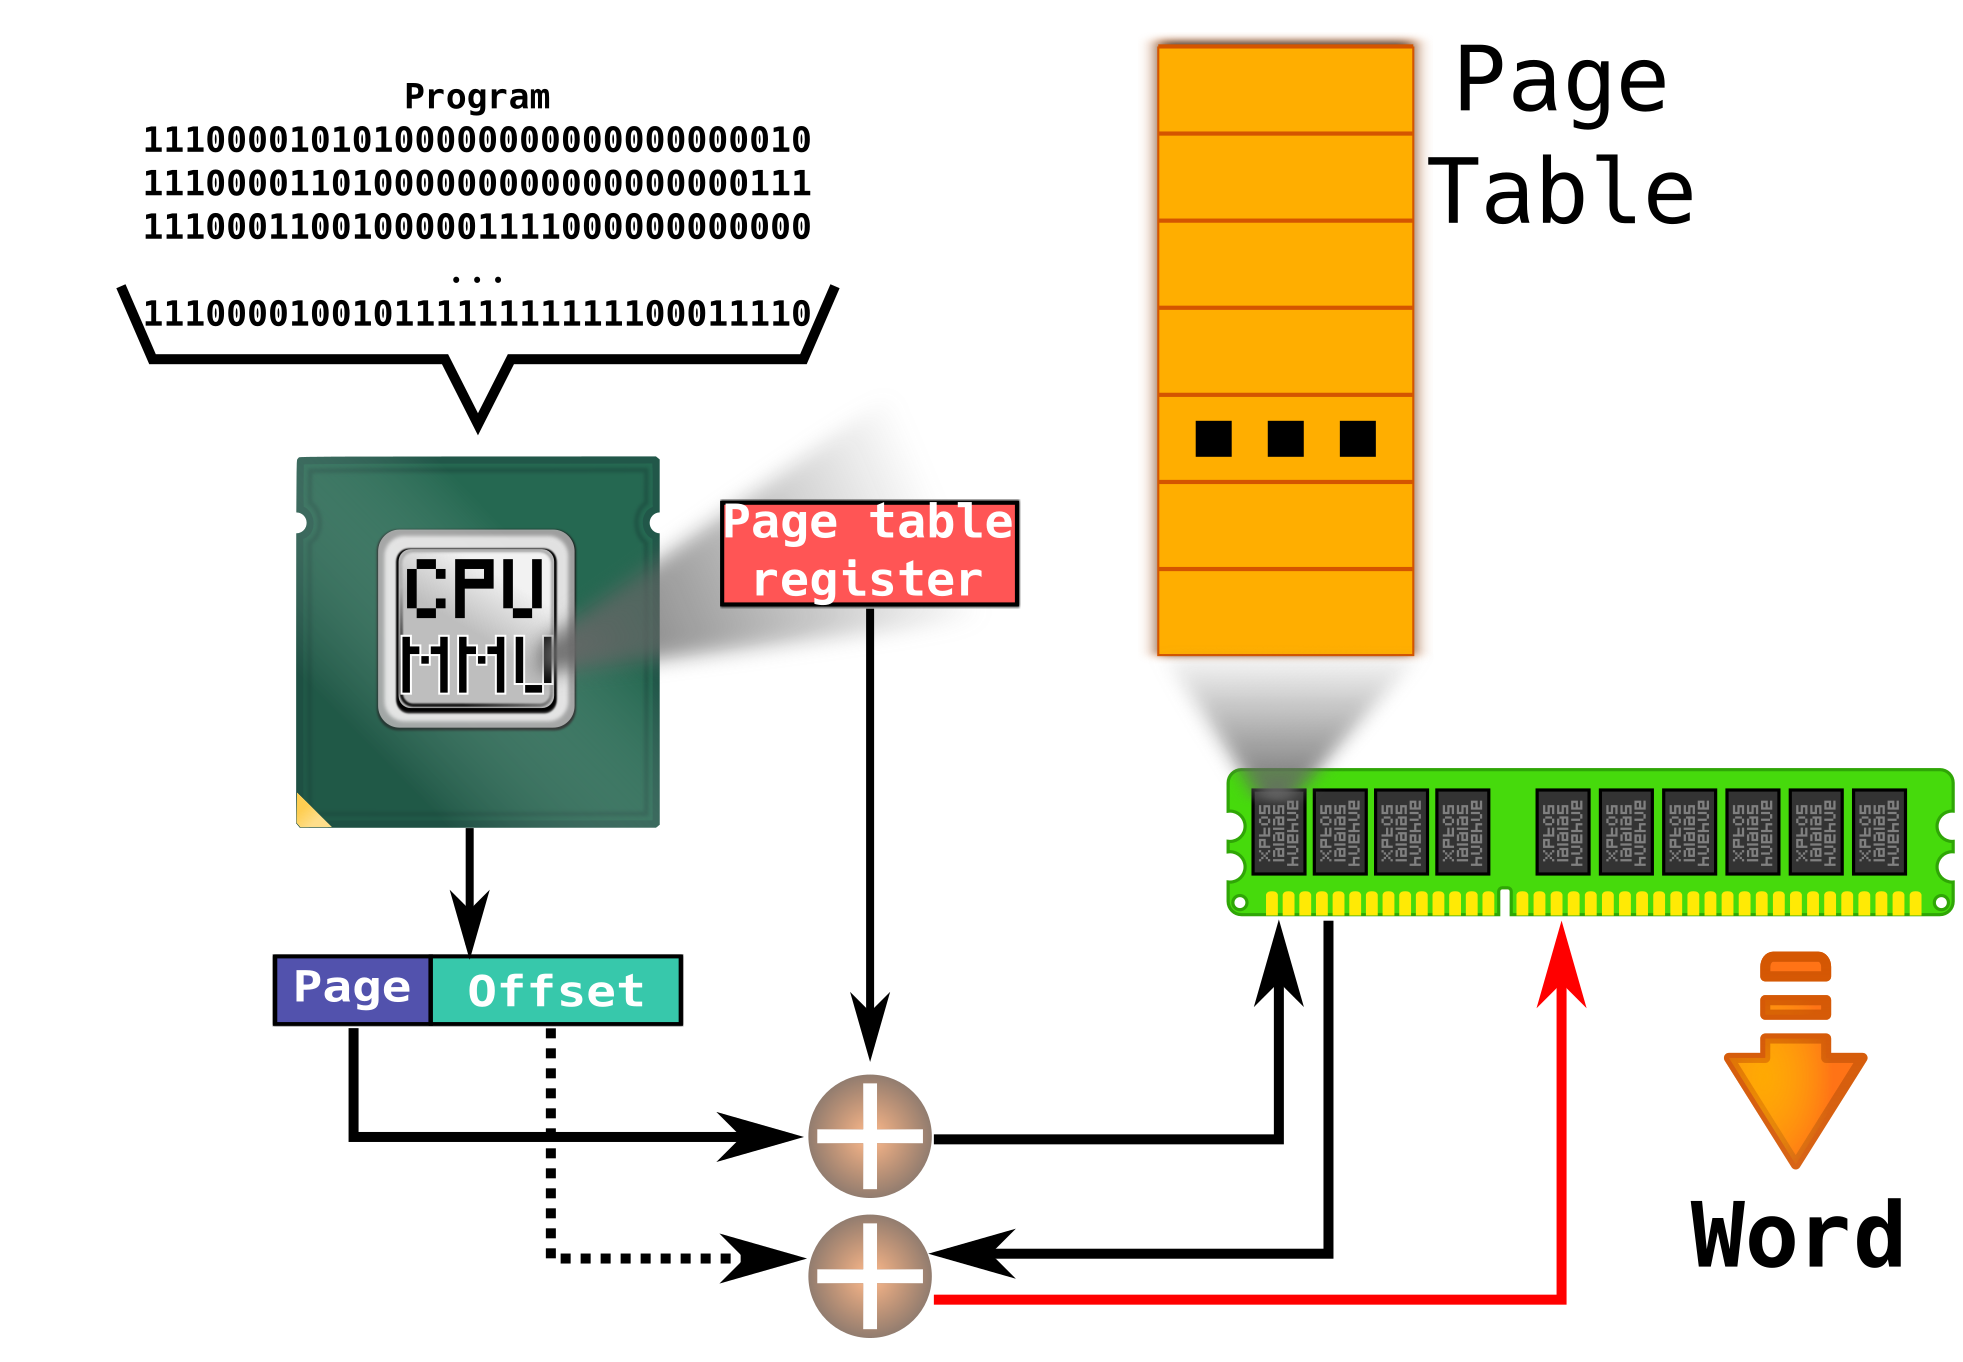
\includegraphics[width=0.9\textwidth, keepaspectratio=true]{images/mmu_f.png}
  \end{figure}
\end{frame}

\begin{frame}{Memory Management}{Overview}
  \begin{figure}[ht]
    \centering
    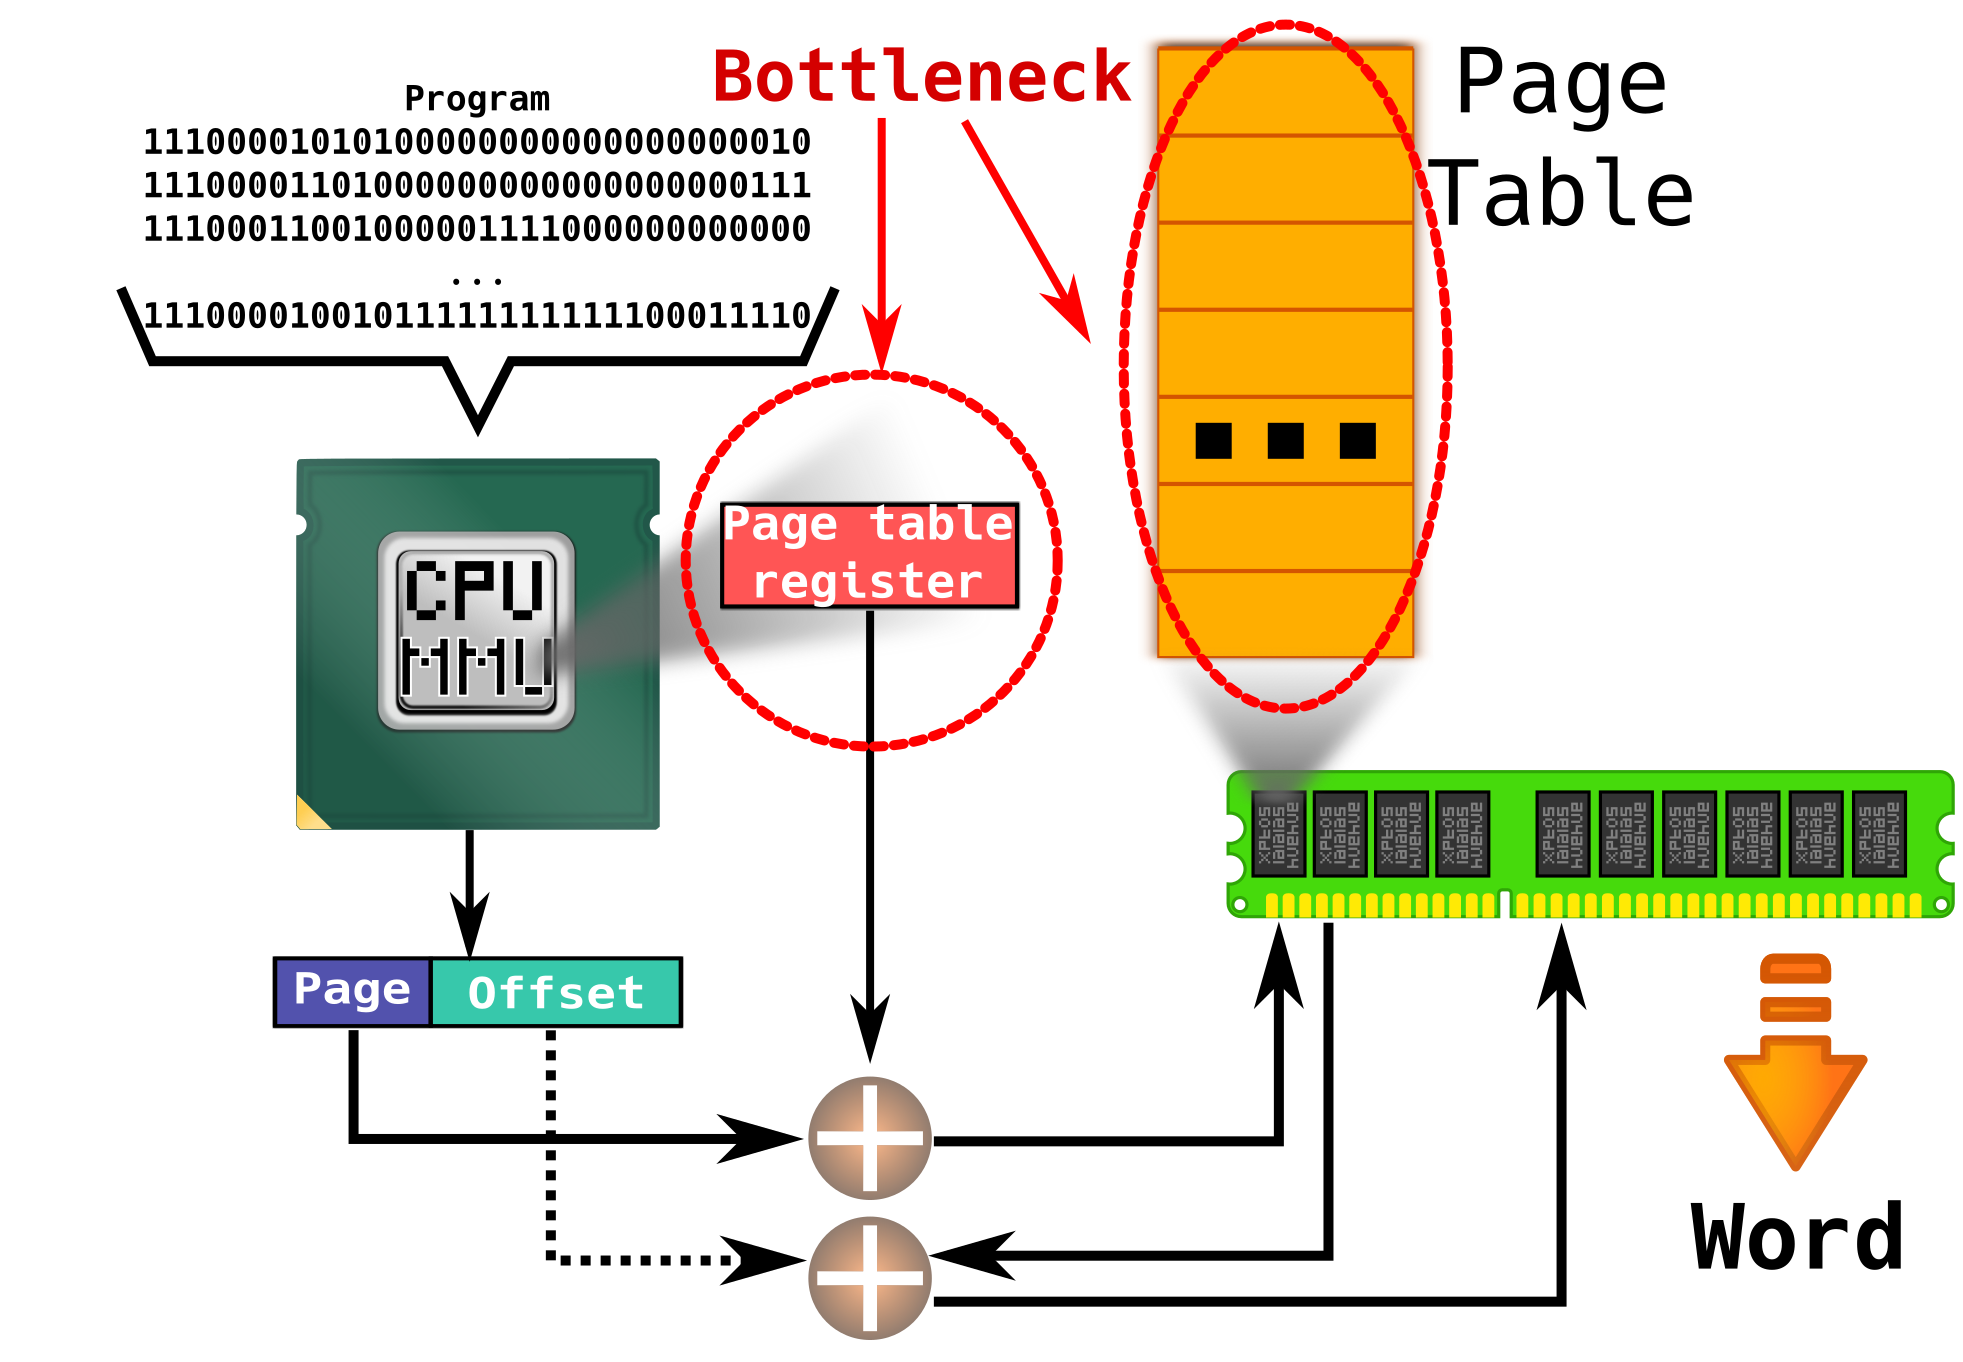
\includegraphics[width=0.9\textwidth, keepaspectratio=true]{images/tlb_a.png}
  \end{figure}
\end{frame}

\begin{frame}{Memory Management}{Overview}
  \begin{figure}[ht]
    \centering
    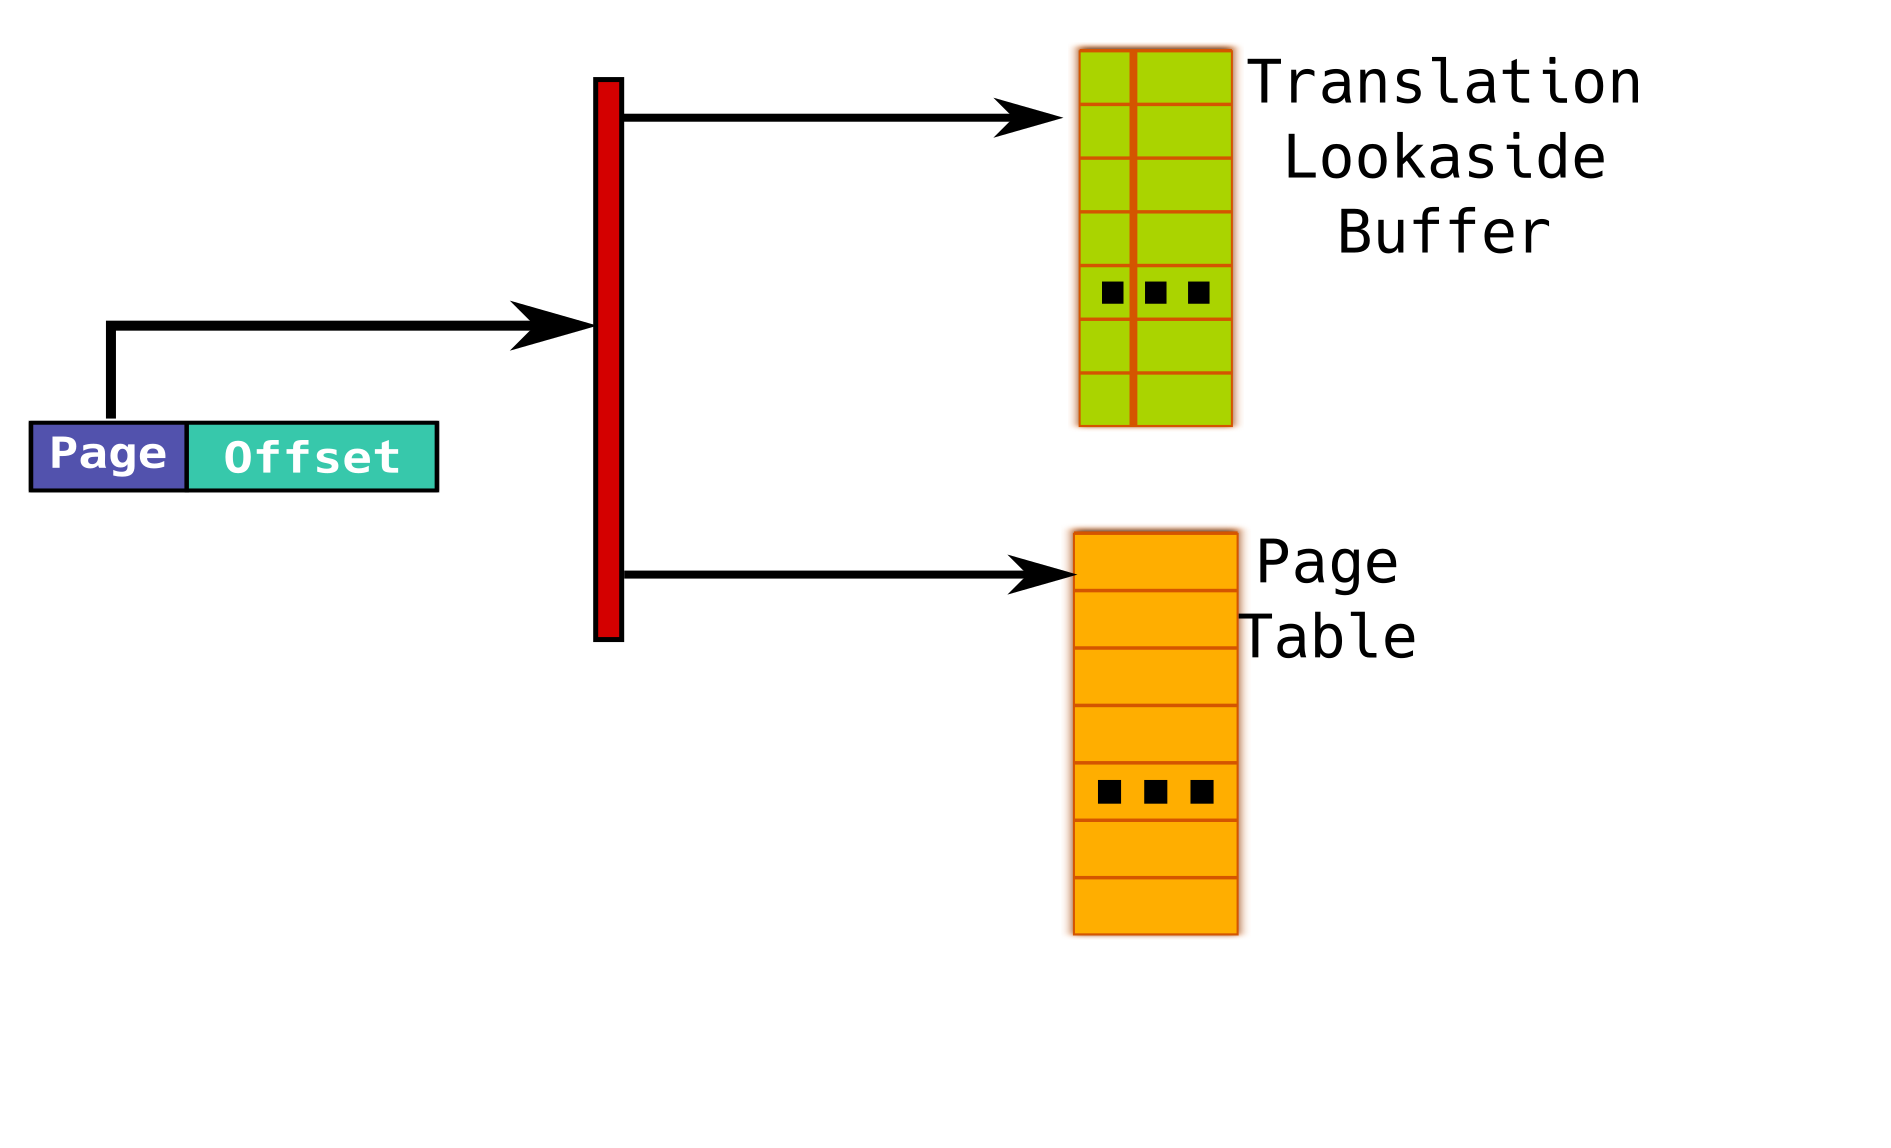
\includegraphics[width=0.9\textwidth, keepaspectratio=true]{images/tlb_b.png}
  \end{figure}
\end{frame}

\begin{frame}{Memory Management}{Overview}
  \begin{figure}[ht]
    \centering
    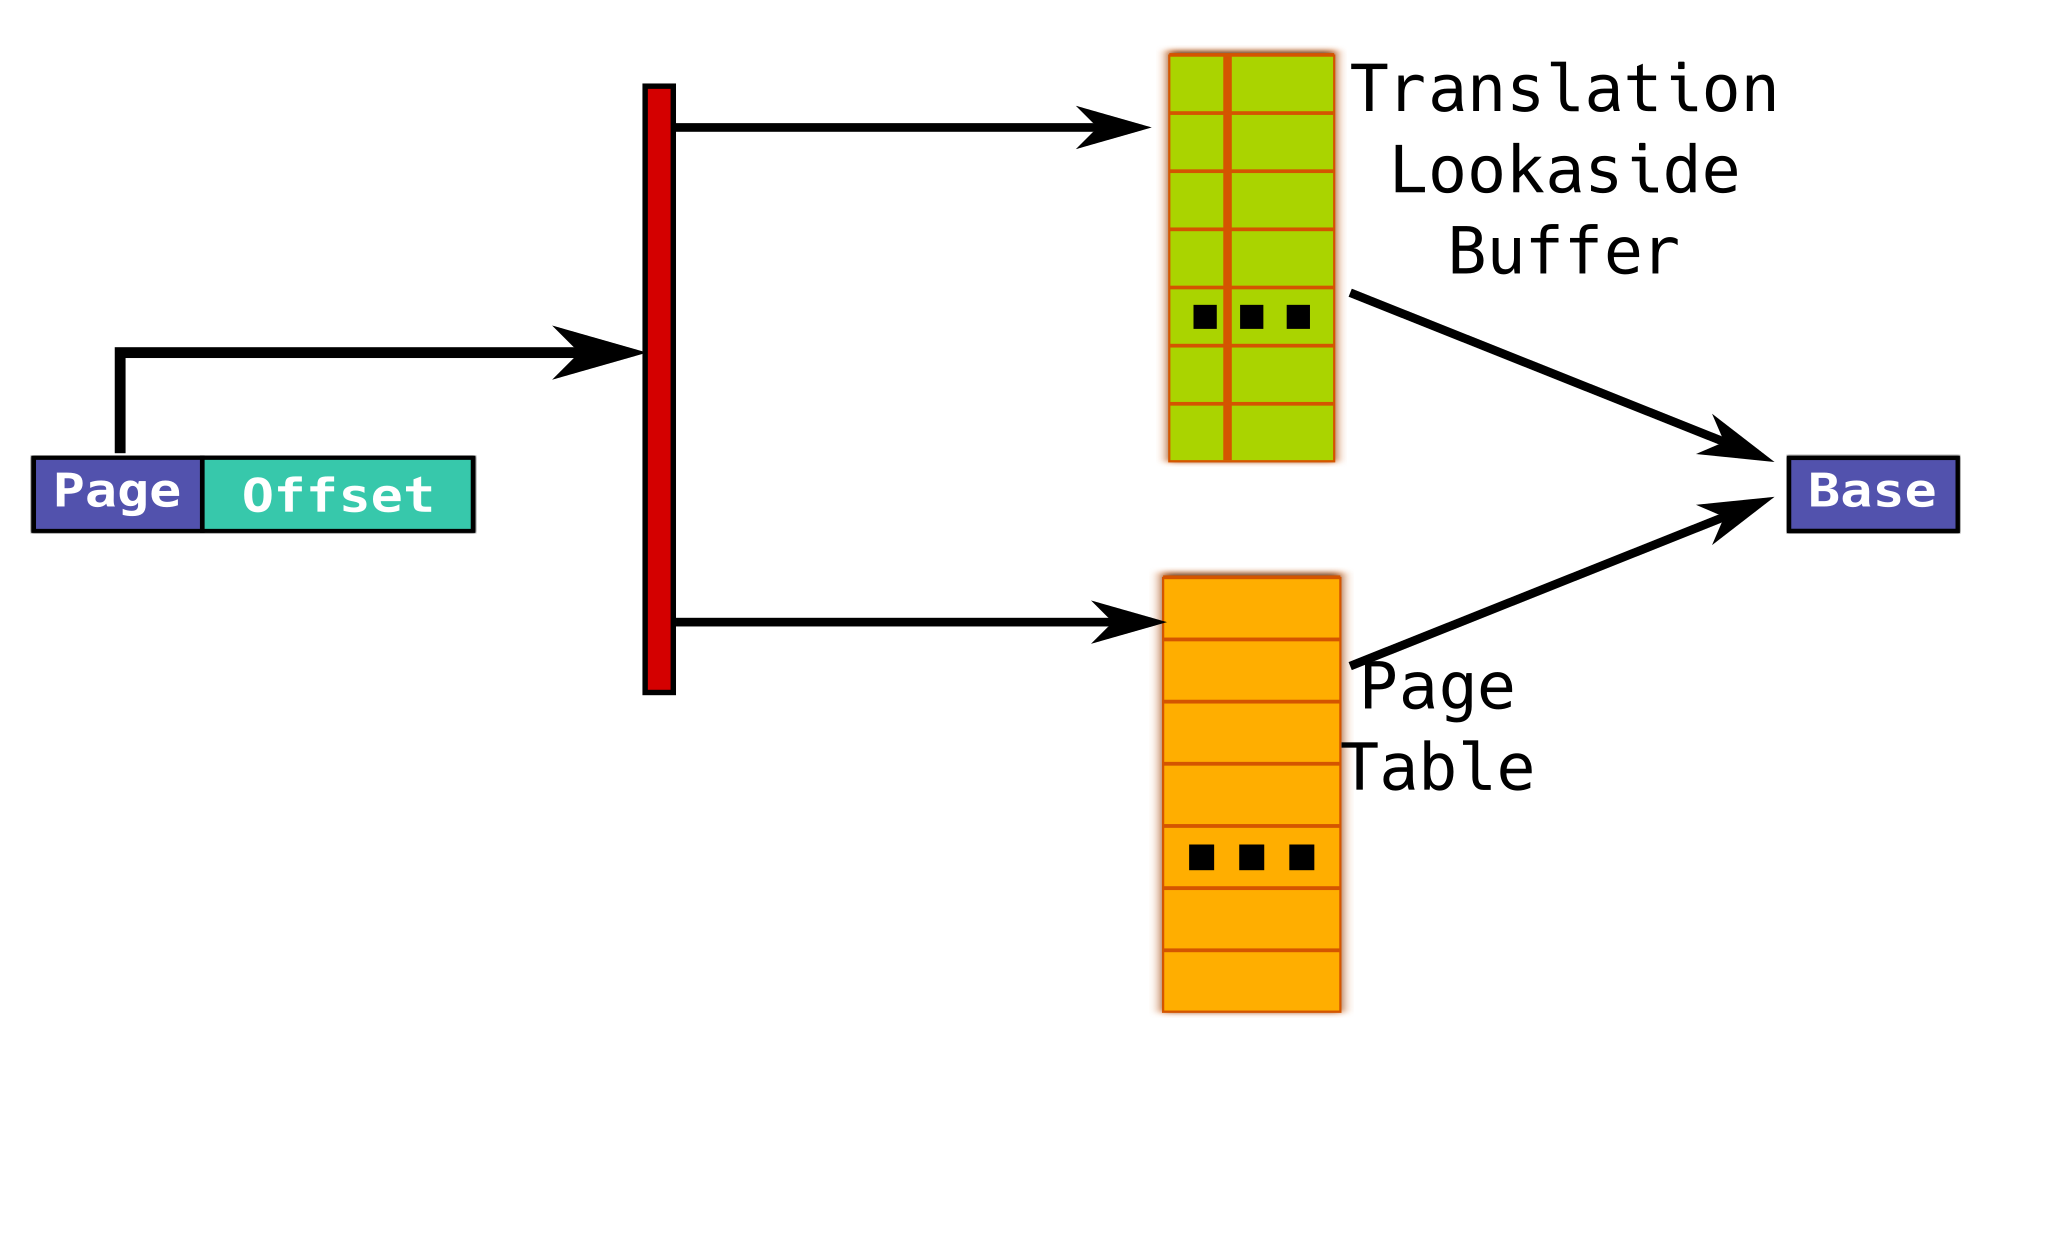
\includegraphics[width=0.9\textwidth, keepaspectratio=true]{images/tlb_c.png}
  \end{figure}
\end{frame}

\begin{frame}{Memory Management}{Overview}
  \begin{figure}[ht]
    \centering
    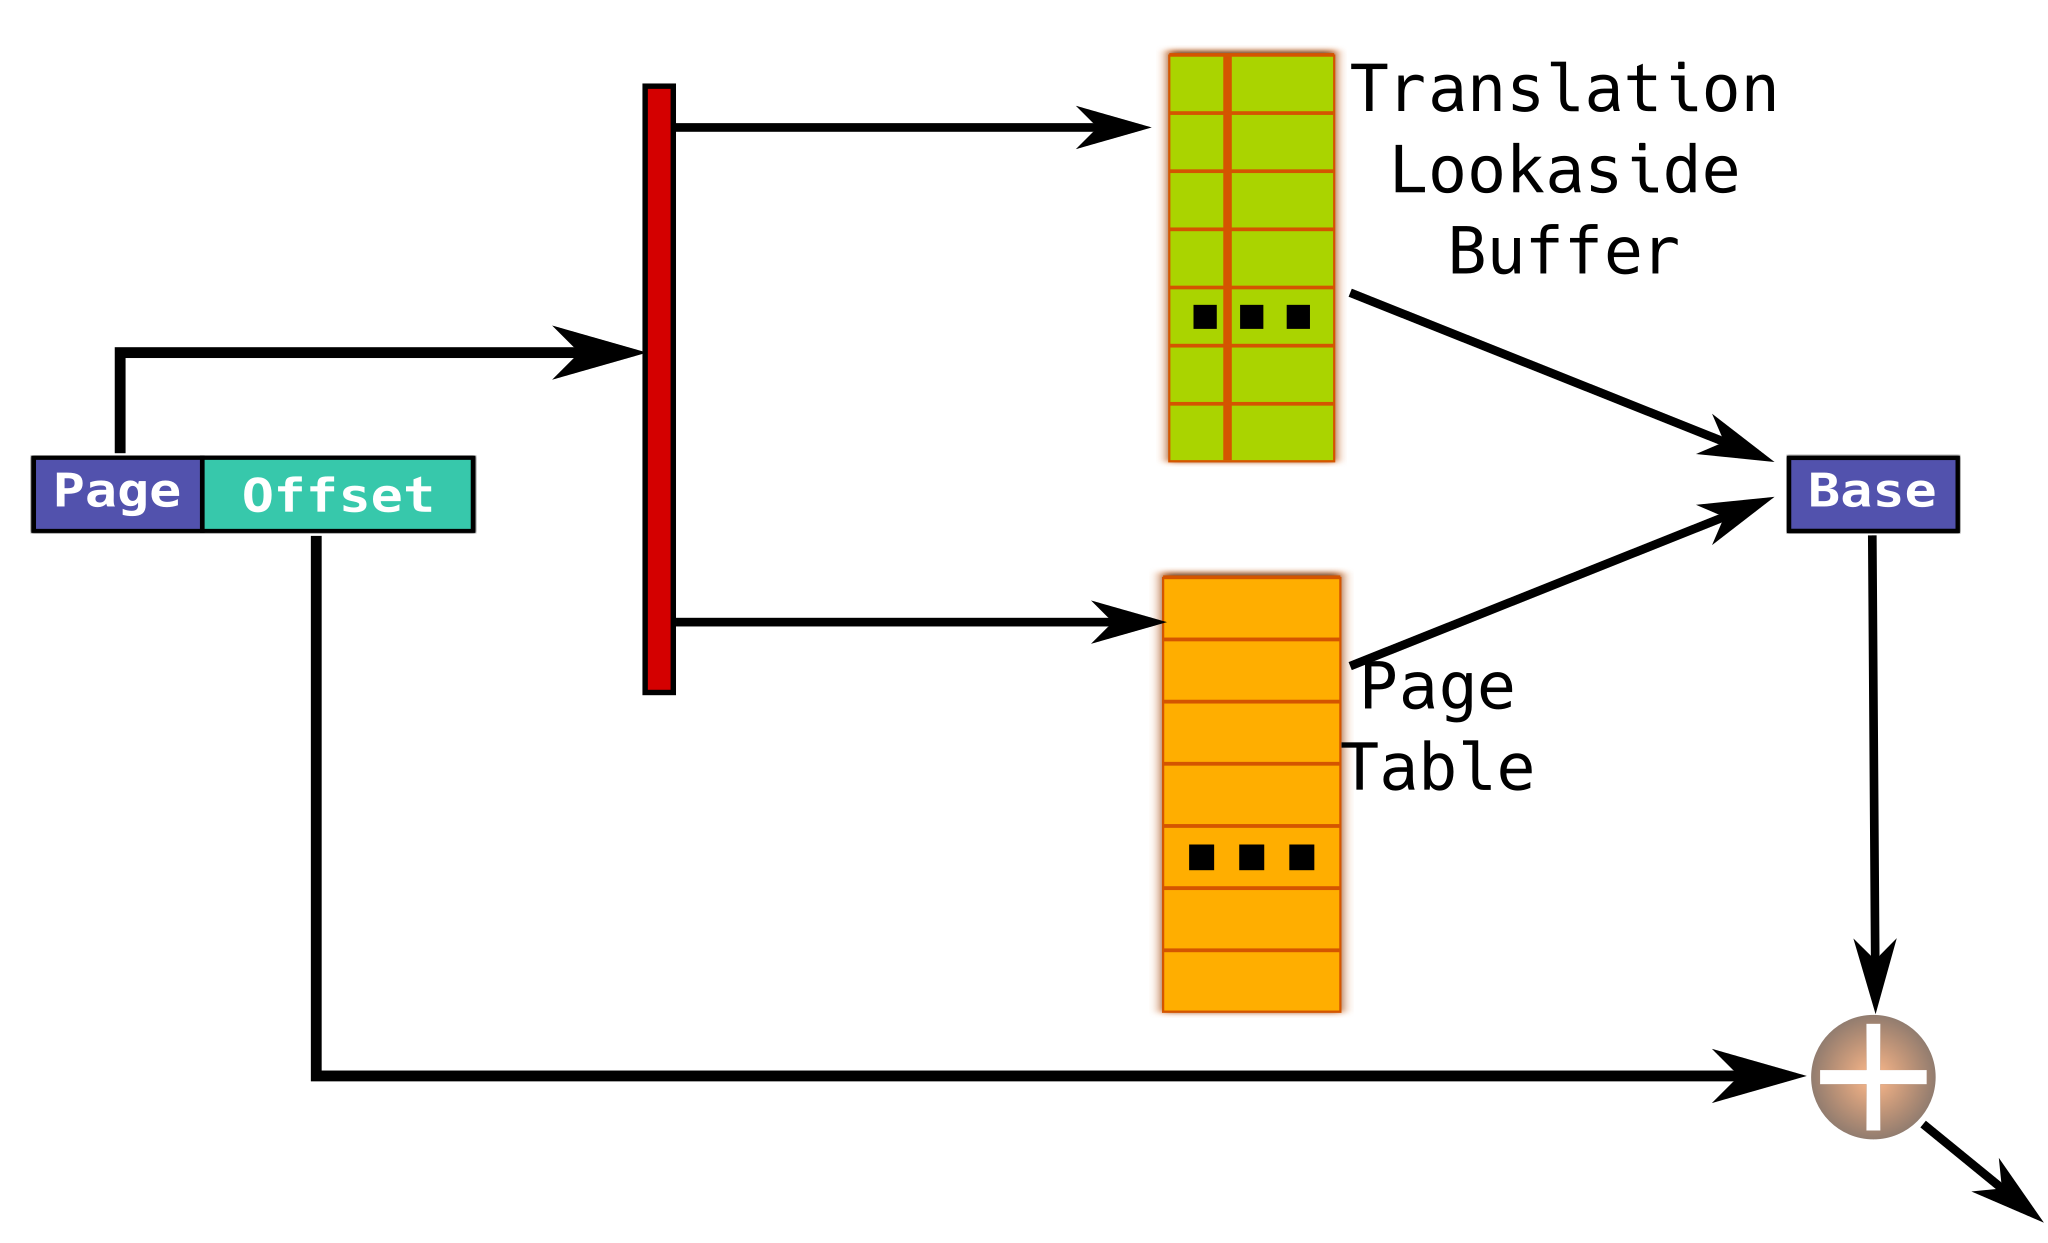
\includegraphics[width=0.9\textwidth, keepaspectratio=true]{images/tlb_d.png}
  \end{figure}
\end{frame}

%-------------------------------------------------------
% Memory centric
%-------------------------------------------------------
\section{Memory Centric}
\begin{frame}{Memory Centric}{}
"What every programmer would like is a private, infinitely large, infinitely
fast memory that is also nonvolatile, that is, does not lose its contents when
the electric power is switched off. While we are at it, why not make it
inexpensive, too? Unfortunately, technology does not provide such memories at
present."\\
Tanenbaum
\end{frame}

\begin{frame}{Memory Centric}{}
  \begin{figure}[ht]
    \centering
    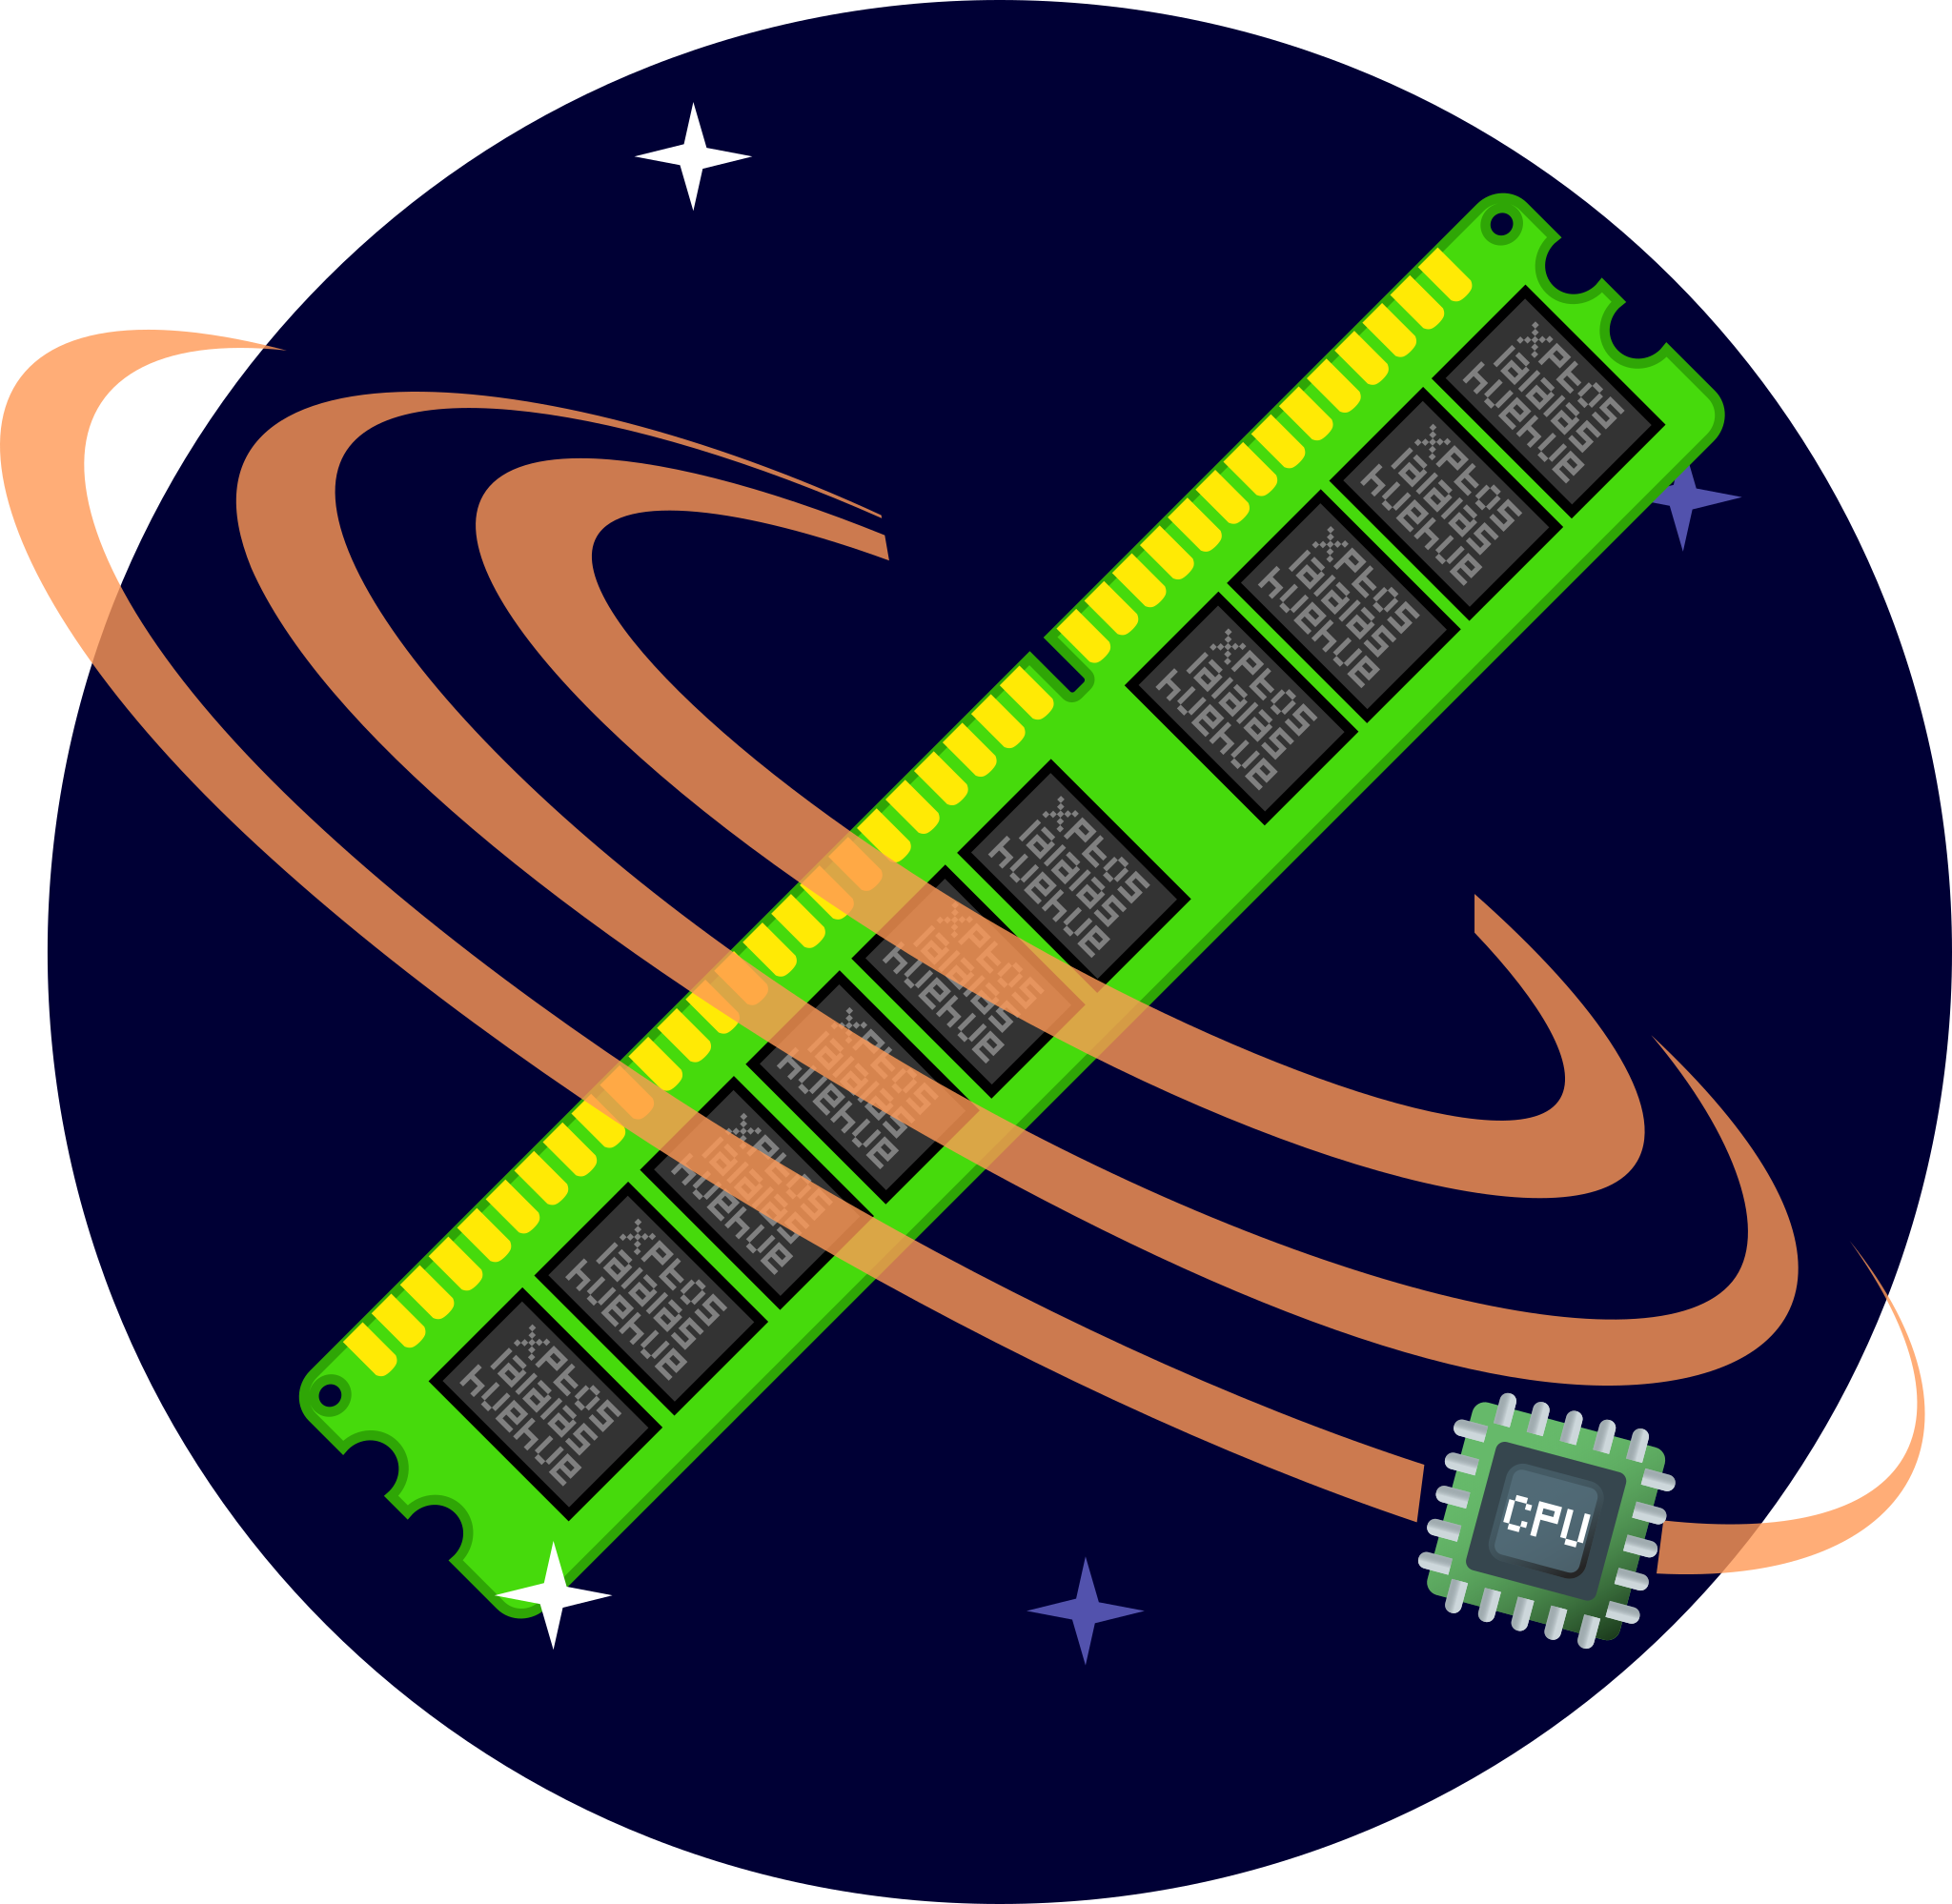
\includegraphics[width=0.7\textwidth, keepaspectratio=true]{images/memory_centric.png}
  \end{figure}
\end{frame}

%-------------------------------------------------------
% Challenges
%-------------------------------------------------------
\section{NVM Challenges}
\begin{frame}{NVM Challenges}{Addressing huge physical memory}
  \textbf{Addressing more physical memory than the size of the virtual space}

  \begin{columns}[T]
    \begin{column}{.2\textwidth}
      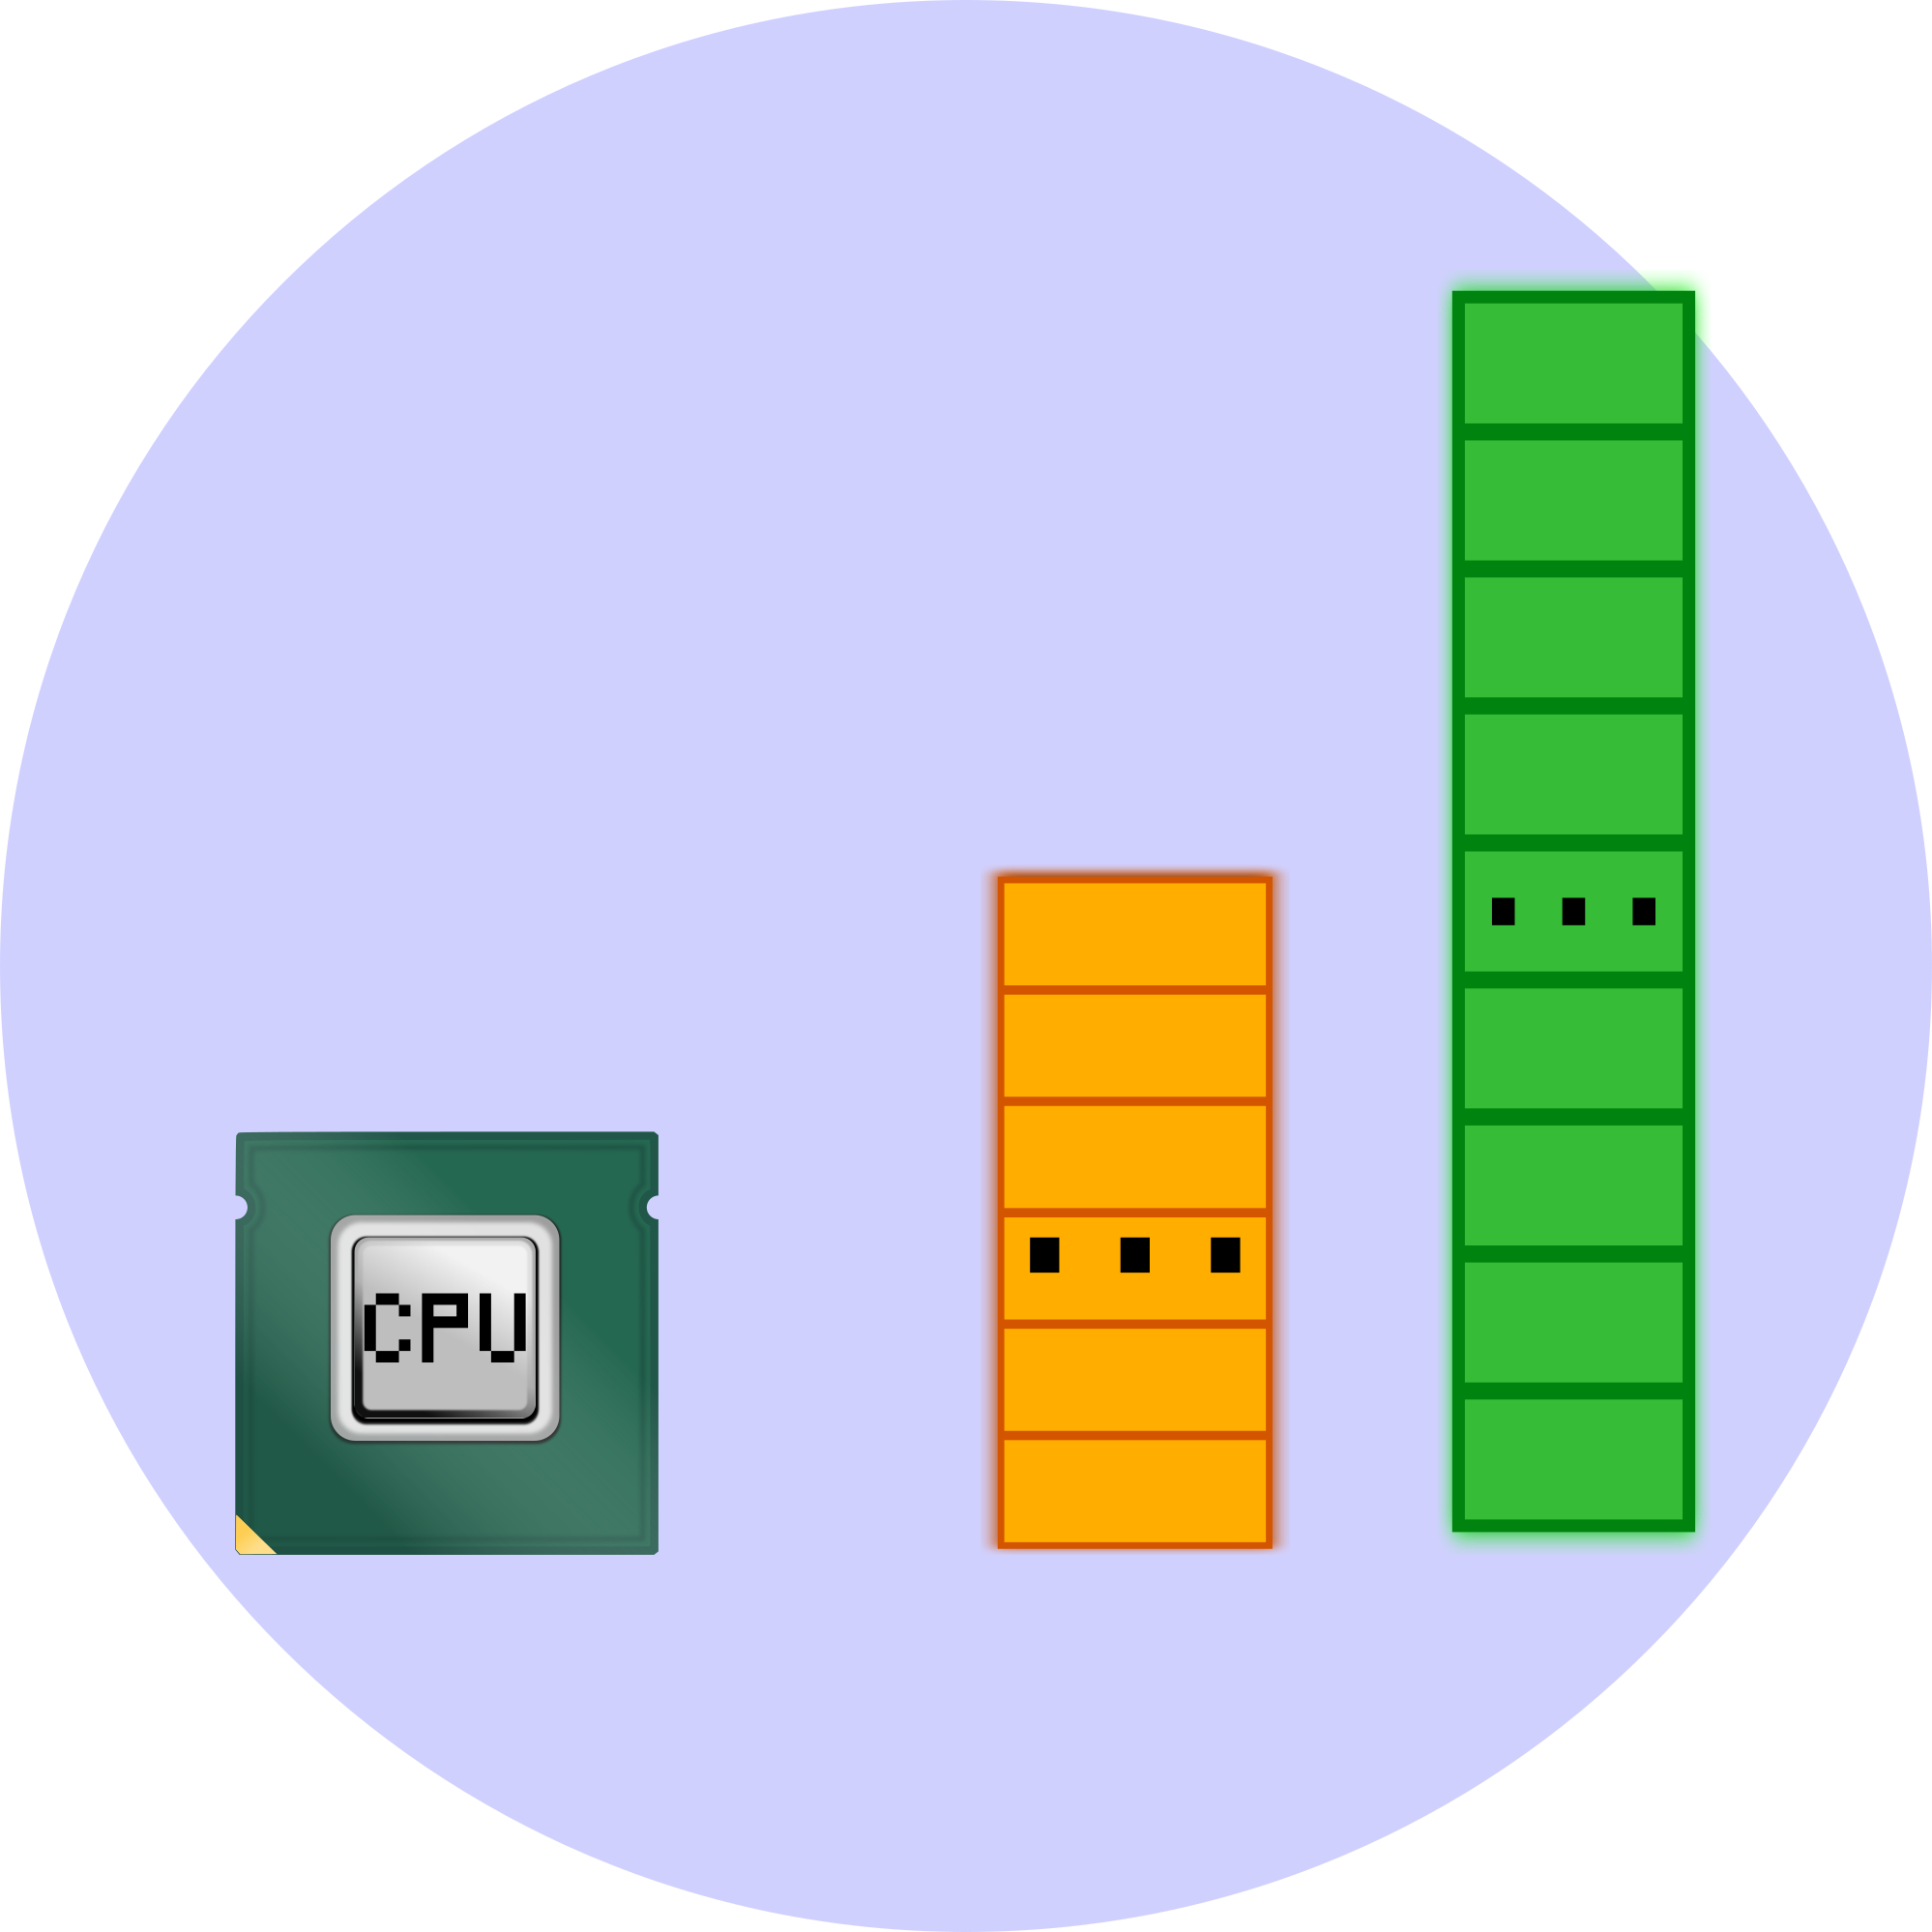
\includegraphics[width=1.8\textwidth, keepaspectratio=true]{images/increase_physical_address.png}
    \end{column} \pause

    \hfill
    \begin{column}{.7\textwidth}
      Possible solution: Increase the number of virtual address (VA) bits \pause
      \begin{itemize}
        \item Increase cache miss in the TLB\pause
        \item Impacts performance, power, production, and cost
      \end{itemize}
    \end{column}
  \end{columns}
\end{frame}

\begin{frame}{NVM Challenges}{Sharing data}
  \textbf{Sharing data across parallel processes}

  \begin{columns}[T]
    \begin{column}{.2\textwidth}
      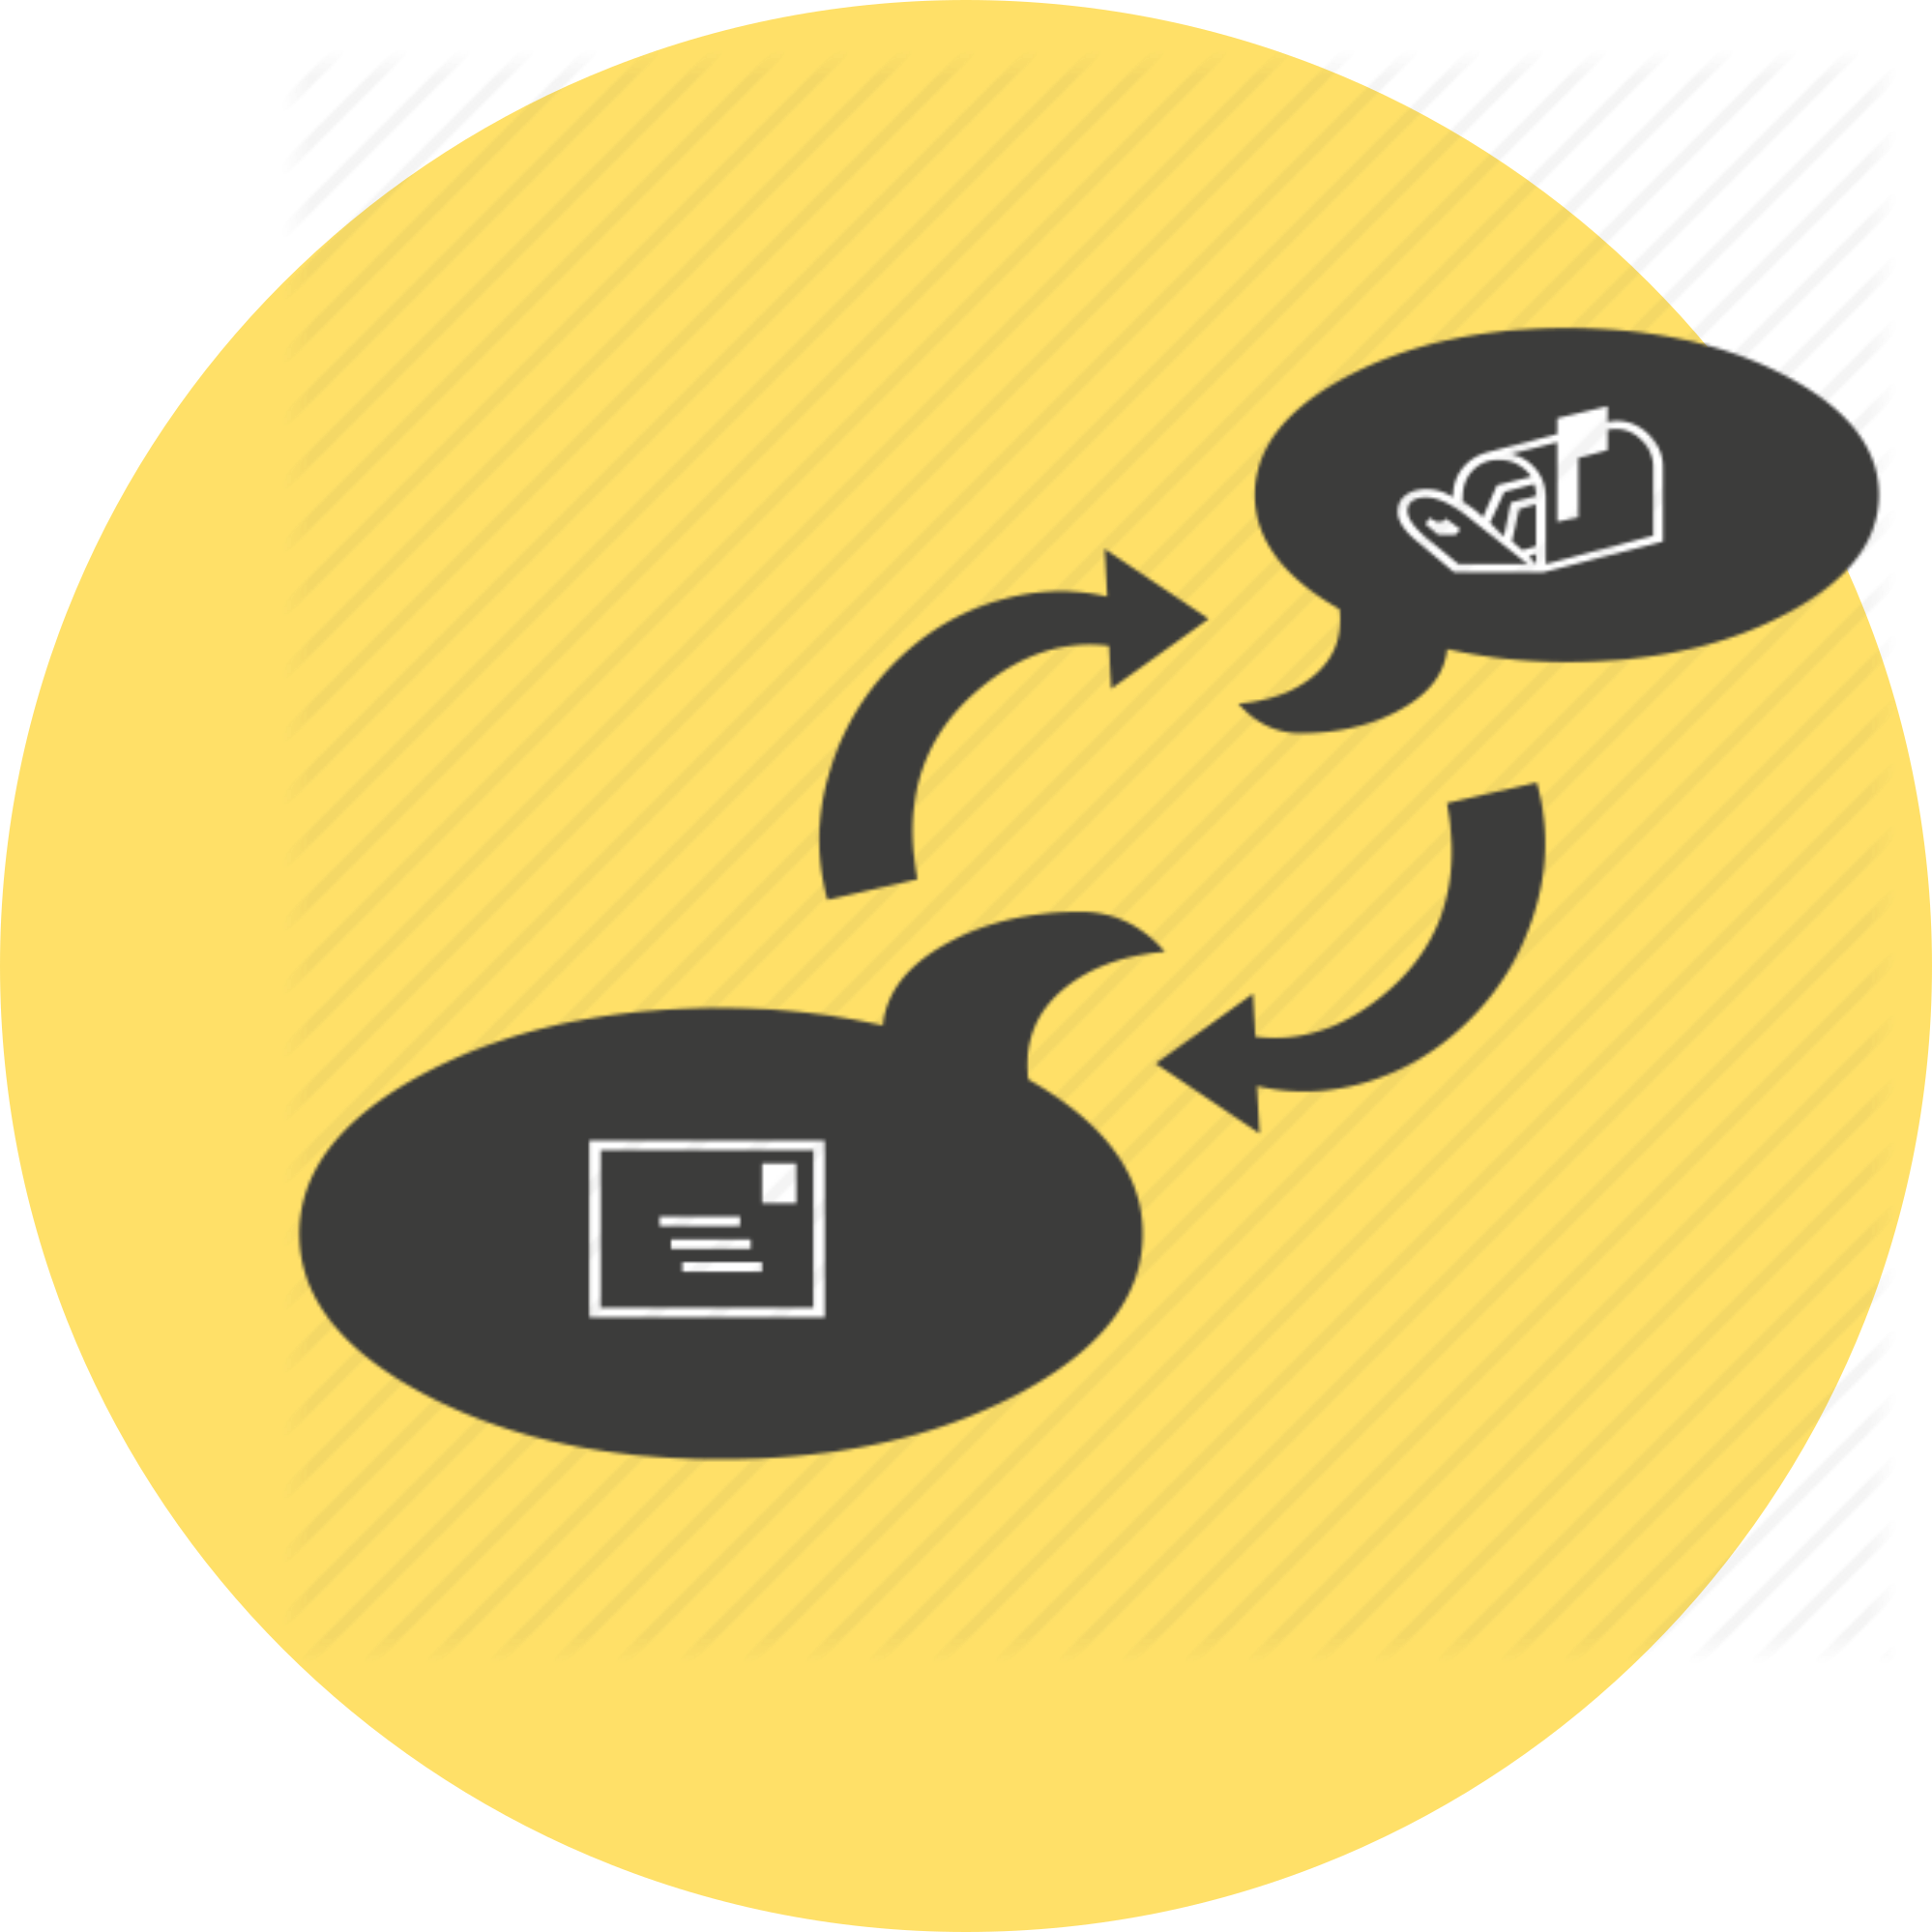
\includegraphics[width=1.7\textwidth, keepaspectratio=true]{images/client_server.png}
    \end{column} \pause

    \hfill
    \begin{column}{.7\textwidth}
      Possible solution: Client-server model \pause
      \begin{itemize}
        \item Modify applications to use client-server interfaces \pause
        \item Communication overhead \pause
      \end{itemize}
      Alternative solution: Shared memory regions \pause
      \begin{itemize}
        \item Current OSs have limitations
      \end{itemize}
    \end{column}

  \end{columns}
\end{frame}

\begin{frame}{NVM Challenges}{Pointer-based Data Structures}
  \textbf{Maintaining Pointer-based Data Structures}

  \begin{columns}[T]
    \begin{column}{.2\textwidth}
      % TODO: CREATE CLIENT-SERVER IMAGE
      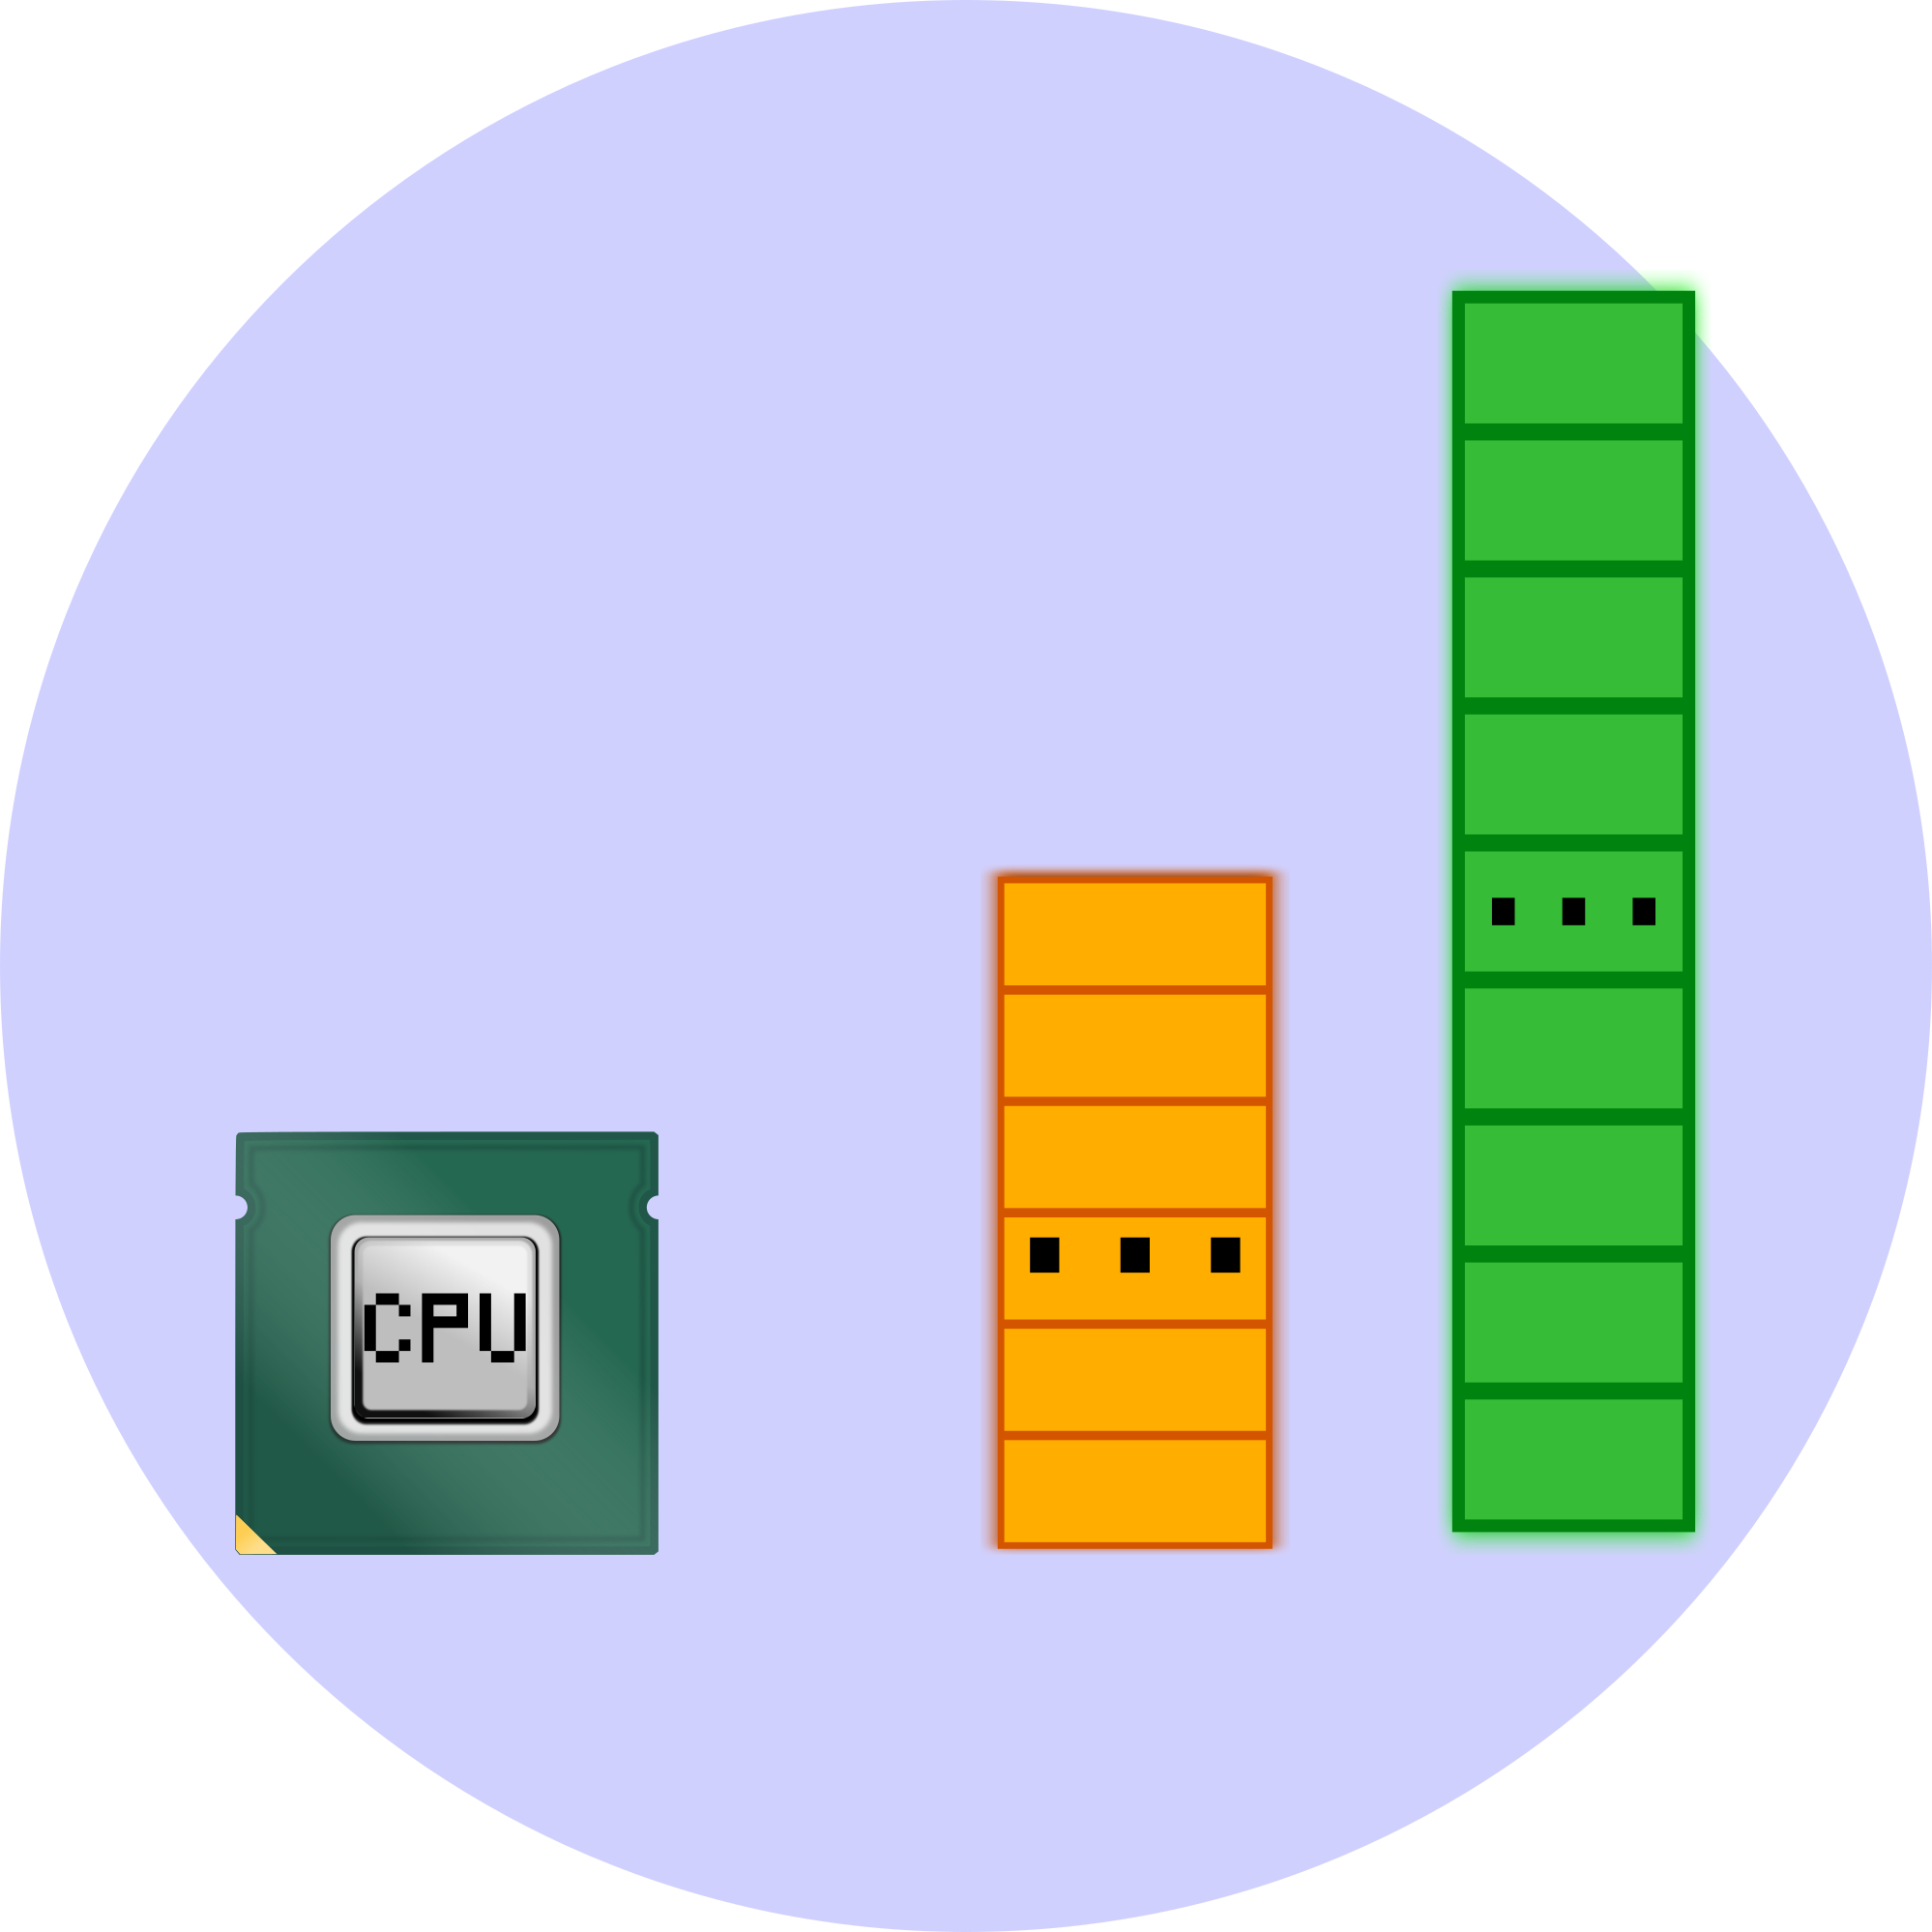
\includegraphics[width=1.7\textwidth, keepaspectratio=true]{images/increase_physical_address.png}
    \end{column} \pause

    \hfill
    \begin{column}{.7\textwidth}
      Possible solution: Special pointers \pause
      \begin{itemize}
        \item Awkward programming techniques
      \end{itemize}
    \end{column}

  \end{columns}
\end{frame}

%-------------------------------------------------------
% SpaceJMP
%-------------------------------------------------------
\section{SpaceJMP}

\begin{frame}{What is SpaceJMP?}{SpaceJMP}
  \begin{itemize}
    \item A set of APIs \pause
    \item OS memory management strategies \pause
    \item Extra memory protection and checkings in the compiler
  \end{itemize}
\end{frame}

\begin{frame}{SpaceJMP and NVM challeges}{Addressing huge physical memory}
  \textbf{Addressing more physical memory than the size of the virtual space}
  \pause
  \begin{itemize}
    \item Decoupling Virtual Address Space \pause
    \item Process can create different Address Spaces
  \end{itemize}
\end{frame}

\begin{frame}{SpaceJMP and NVM challeges}{Sharing data}
  \textbf{Sharing data across simultaneously executing processes}
  \pause
  \begin{itemize}
    \item Allowing processes to switch into a shared address space
  \end{itemize}
\end{frame}

\begin{frame}{SpaceJMP and NVM challeges}{Pointer-based Data Structures}
  \textbf{Maintaining Pointer-based Data Structures} \pause
  \begin{itemize}
    \item Can always guarantee the availability of Virtual Address
  \end{itemize}
\end{frame}

%-------------------------------------------------------
% Design
%-------------------------------------------------------
\section{Design}

\begin{frame}{Design}{Two elements}
  \begin{itemize}
    \item Lockable Segment
    \item Multiple Virtual Address Space
  \end{itemize}
\end{frame}

\begin{frame}{Design}{Lockable Segment}
  What is a Lockable Segment in SpaceJMP? \pause
  \begin{itemize}
    \item Single, contiguous area of virtual memory containing code and data \pause
    \item Fixed virtual start address and size \pause
    \item Metadata describing how to access content in memory \pause
    \item Mapping from virtual address to physical frame \pause
    \item Associated access rights
  \end{itemize}
\end{frame}

\begin{frame}{Design}{Lockable Segment}
  \begin{block}{Important feature}
    All segments are lockable. In order to switch into an address space, the OS
    must acquire a reader/writer lock on each lockable segment in that address
    space.
  \end{block}
\end{frame}

\begin{frame}{Design}{Lockable Segment}
  \begin{figure}[ht]
    \centering
    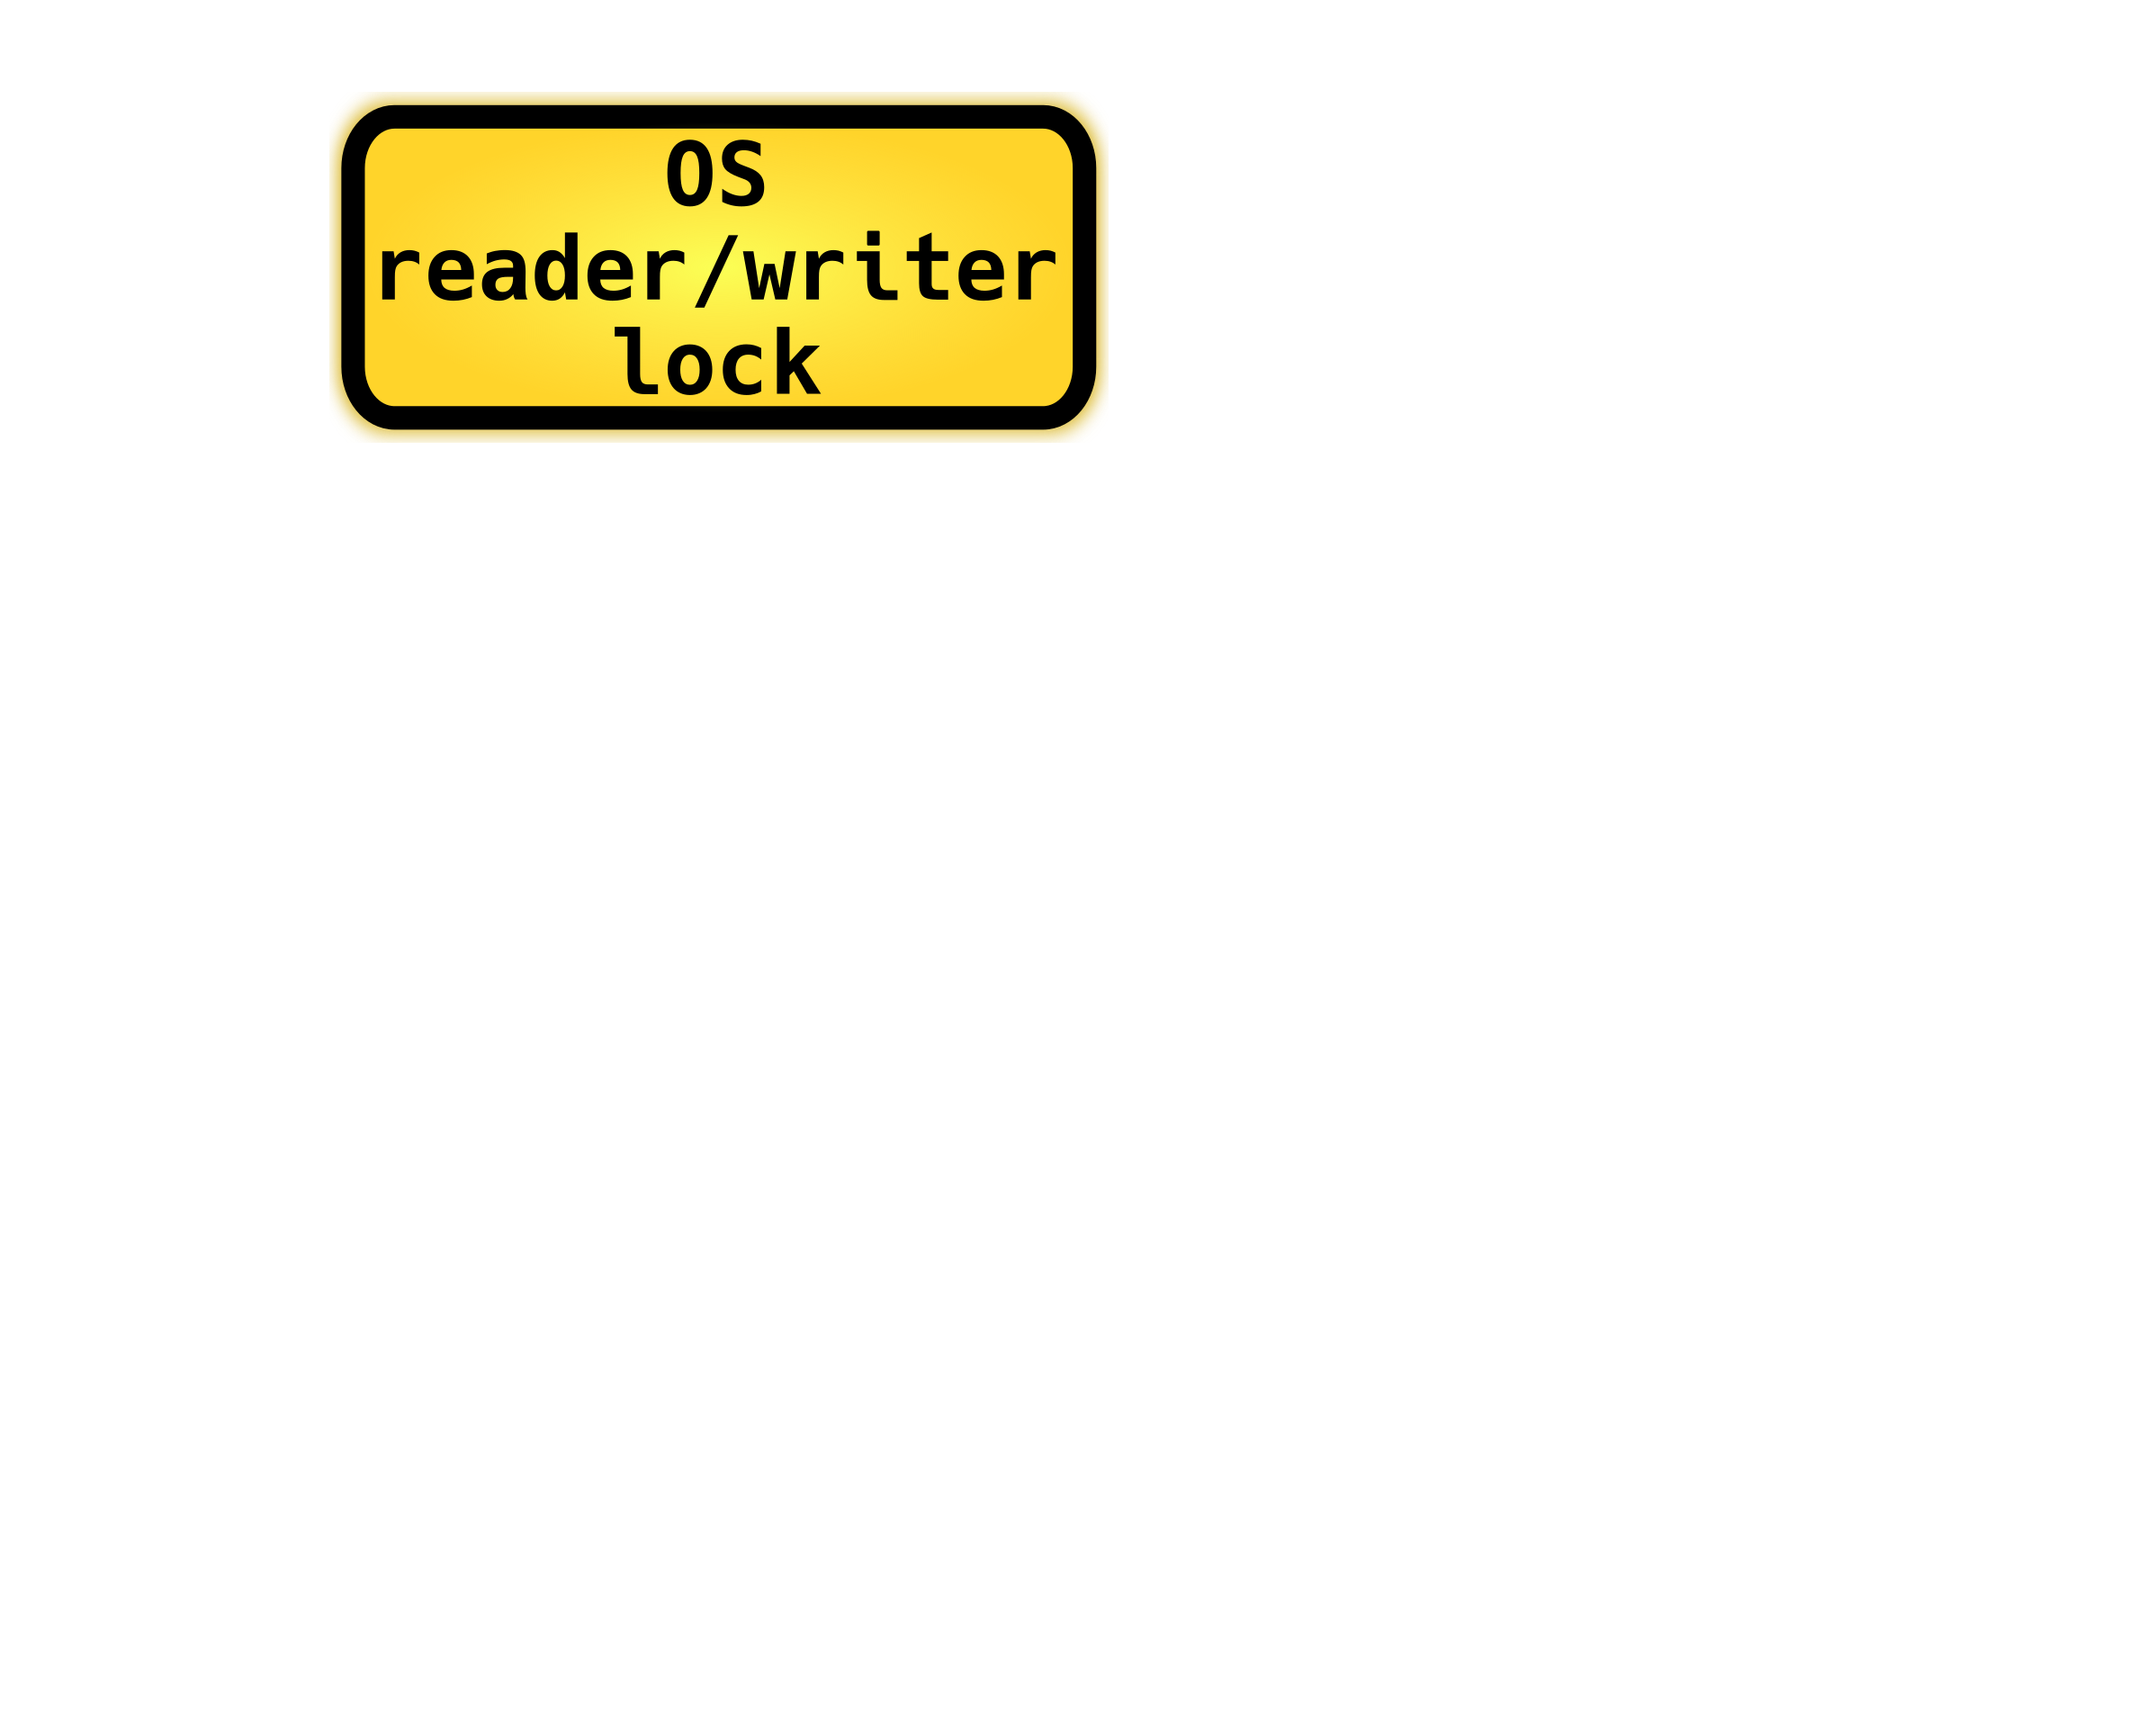
\includegraphics[width=0.7\textwidth, keepaspectratio=true]{images/lockable_segment_a.png}
  \end{figure}
\end{frame}

\begin{frame}{Design}{Lockable Segment}
  \begin{figure}[ht]
    \centering
    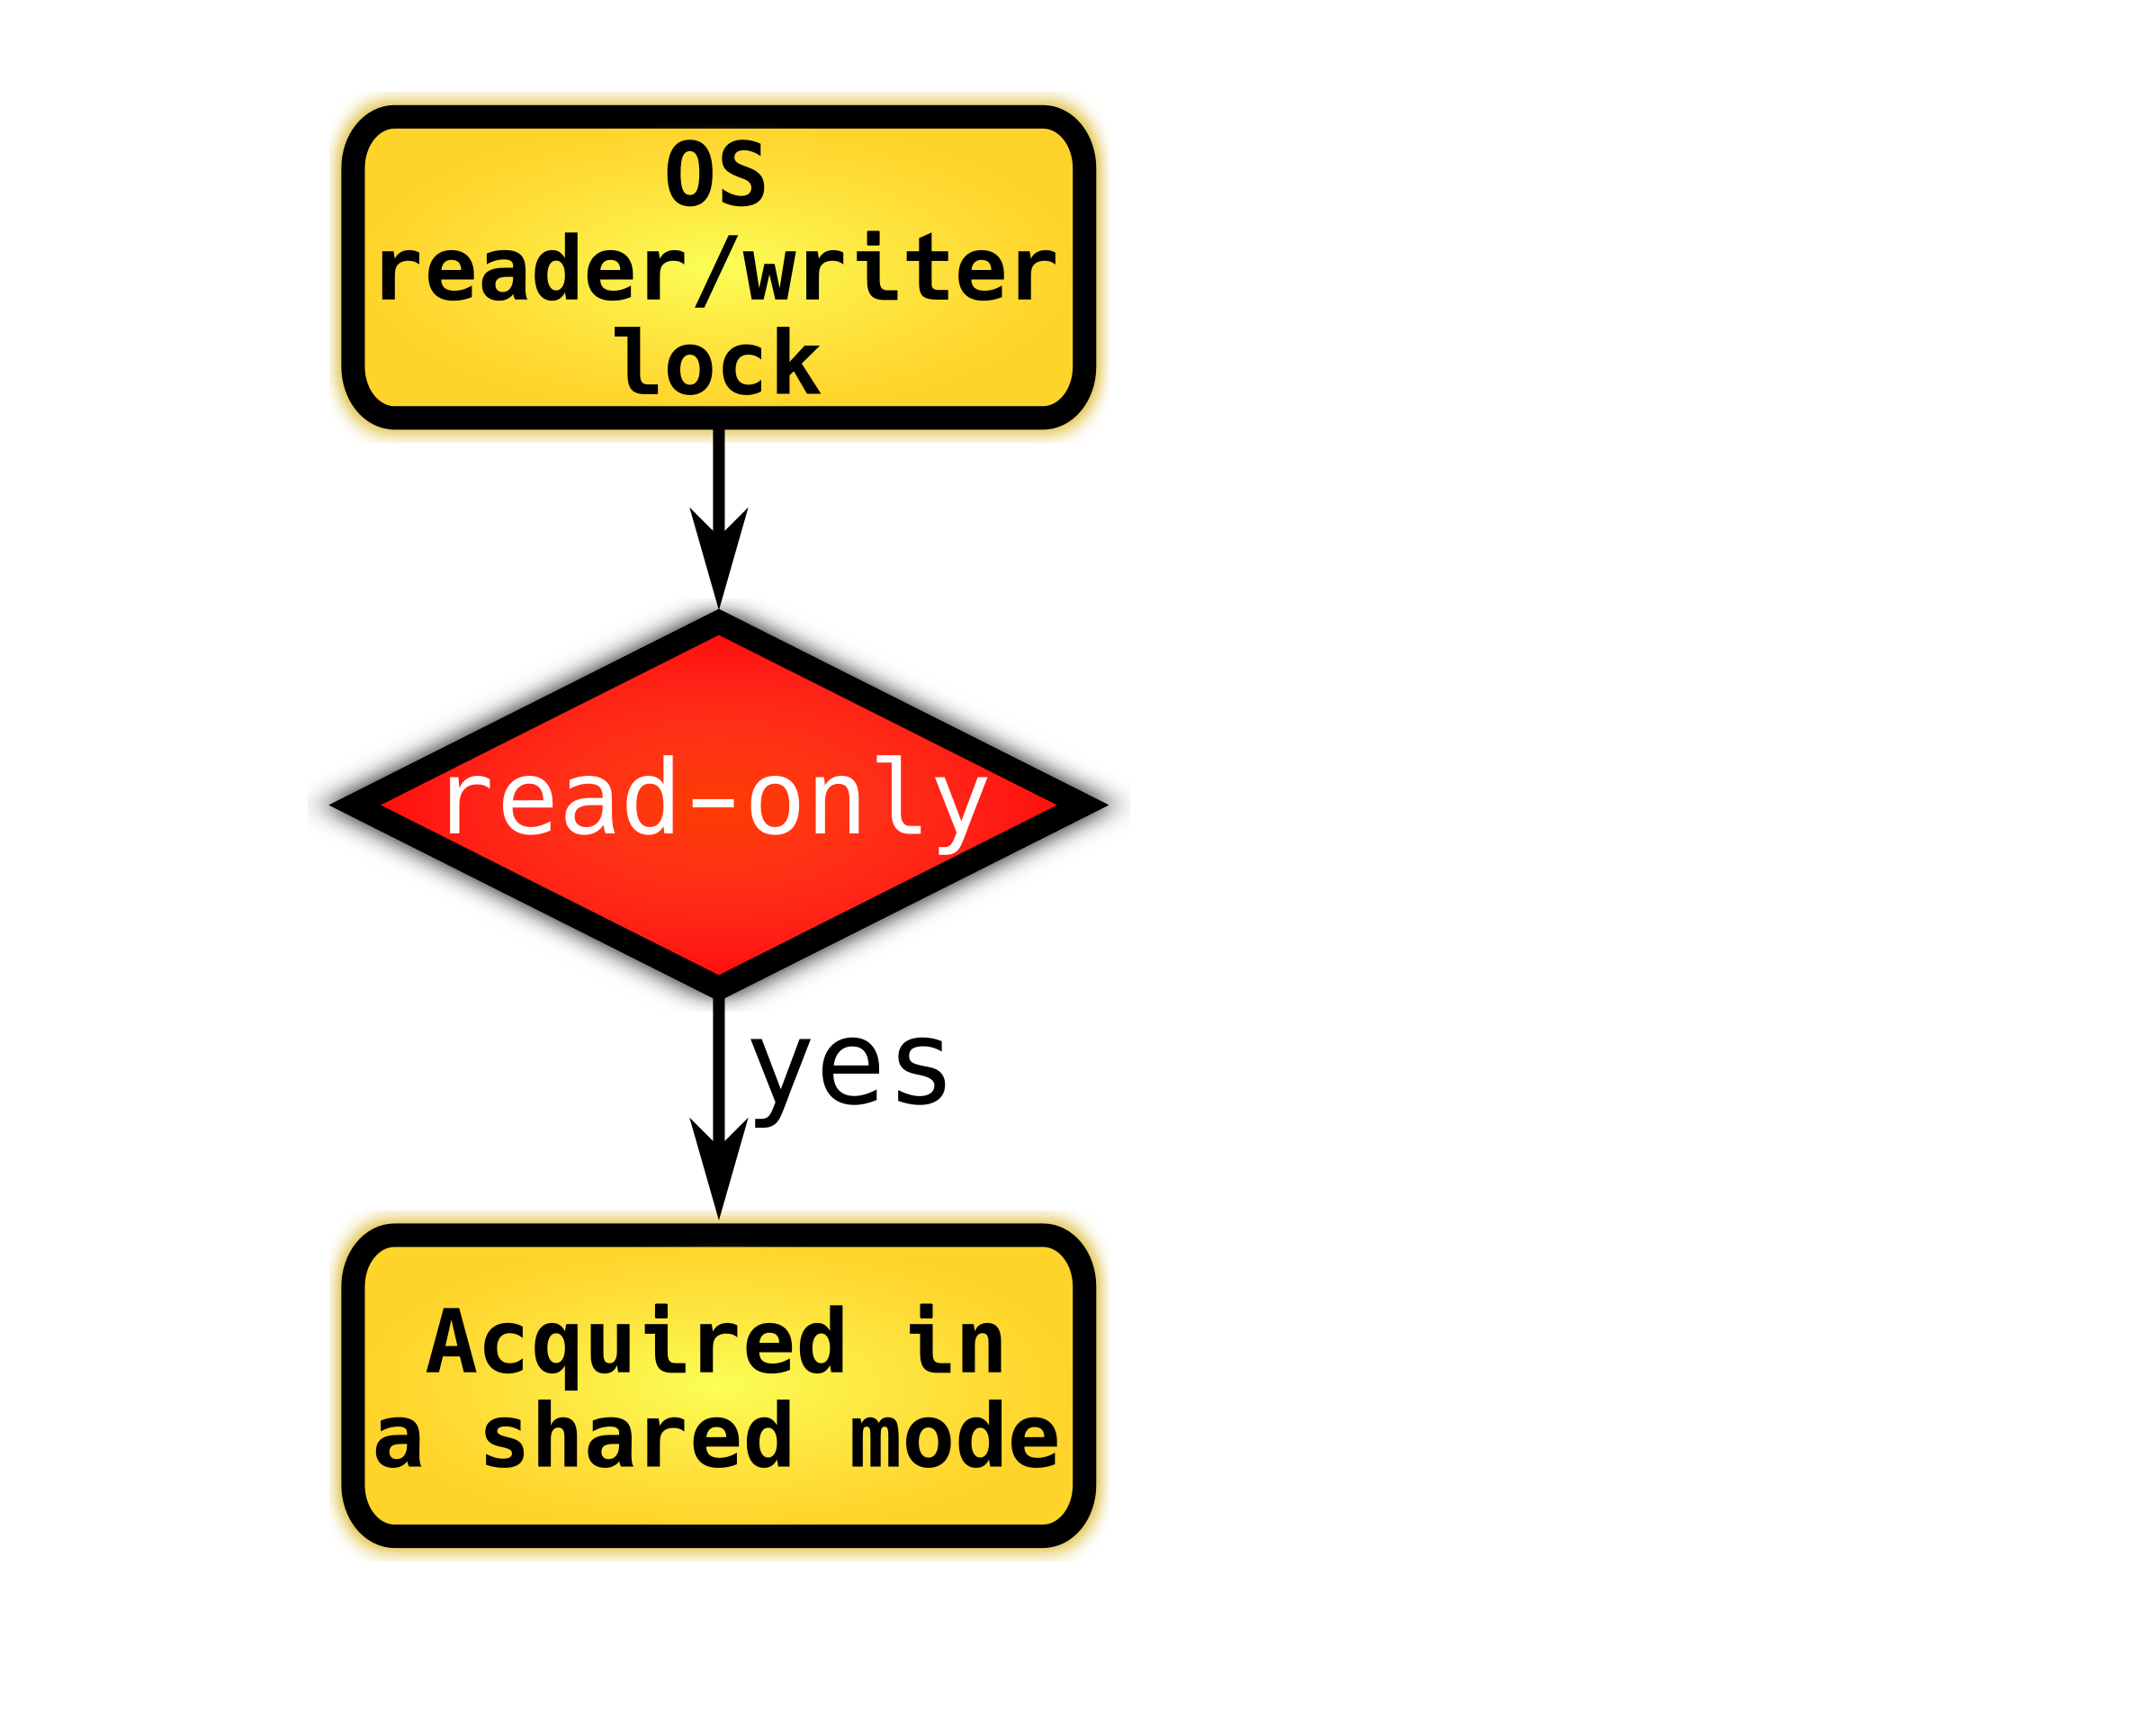
\includegraphics[width=0.7\textwidth, keepaspectratio=true]{images/lockable_segment_b.png}
  \end{figure}
\end{frame}

\begin{frame}{Design}{Lockable Segment}
  \begin{figure}[ht]
    \centering
    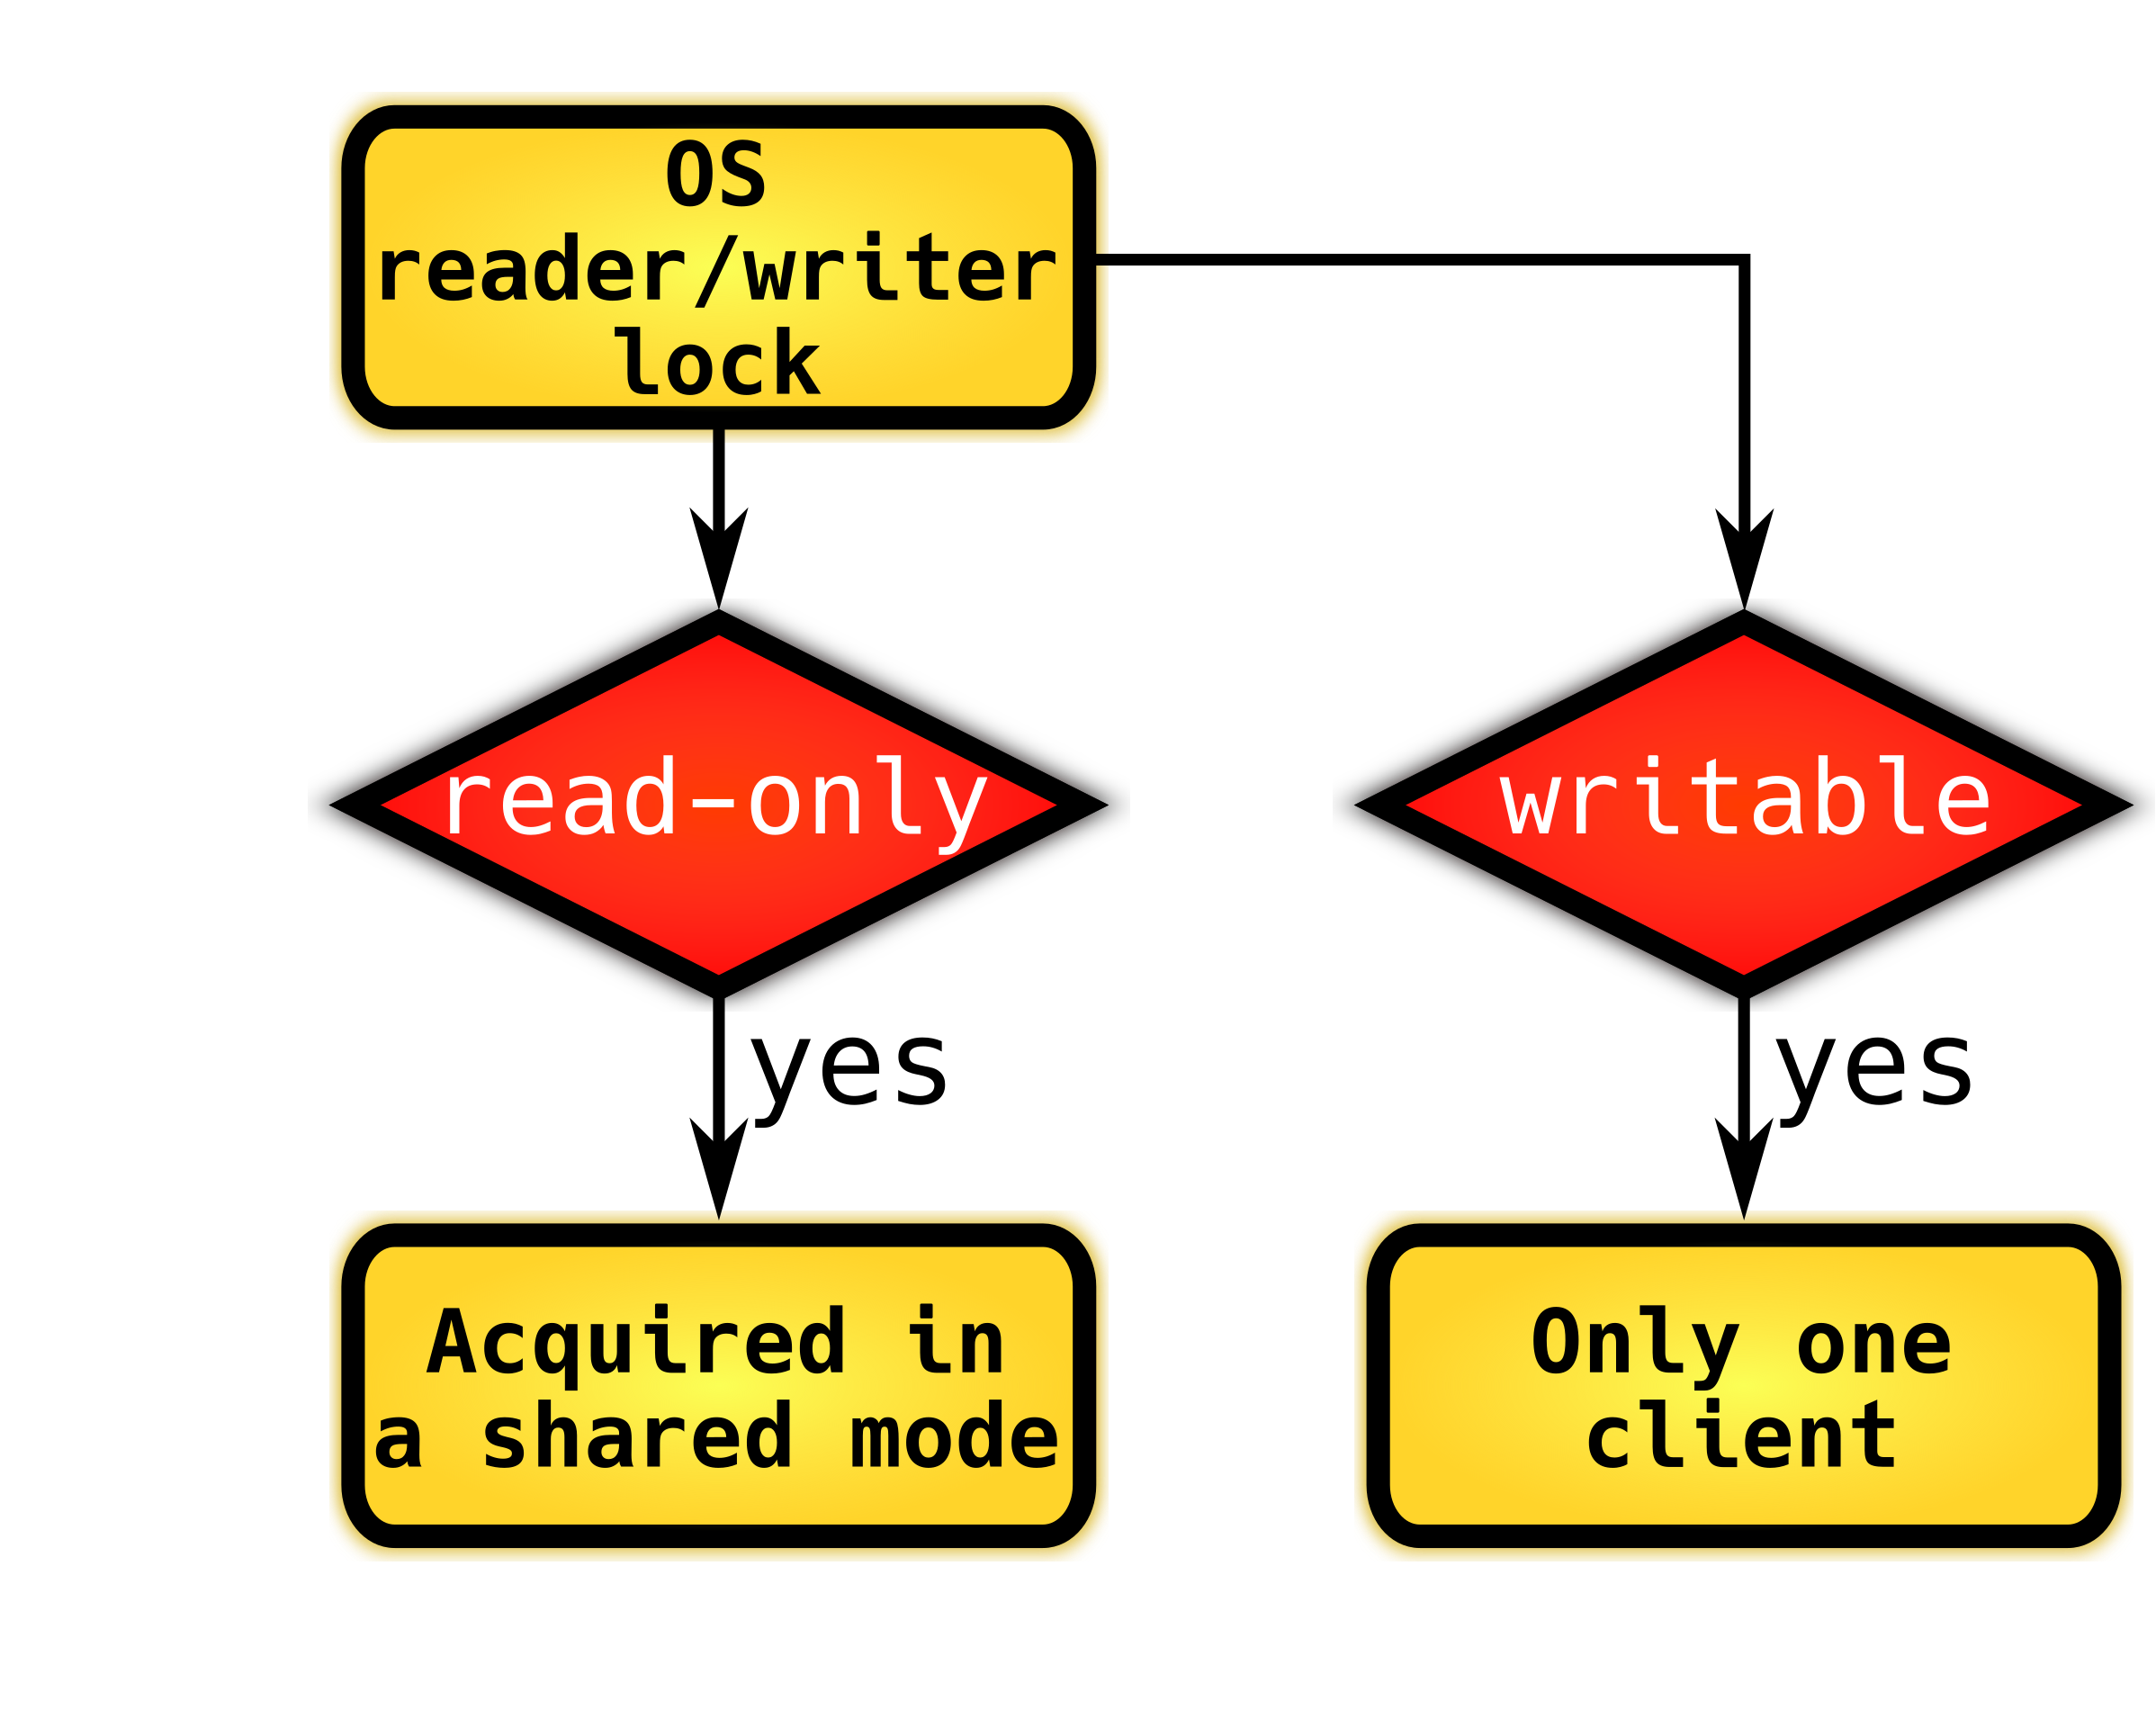
\includegraphics[width=0.7\textwidth, keepaspectratio=true]{images/lockable_segment_c.png}
  \end{figure}
\end{frame}

\begin{frame}{Design}{Multiple Virtual Address Space}
  \begin{figure}[ht]
    \centering
    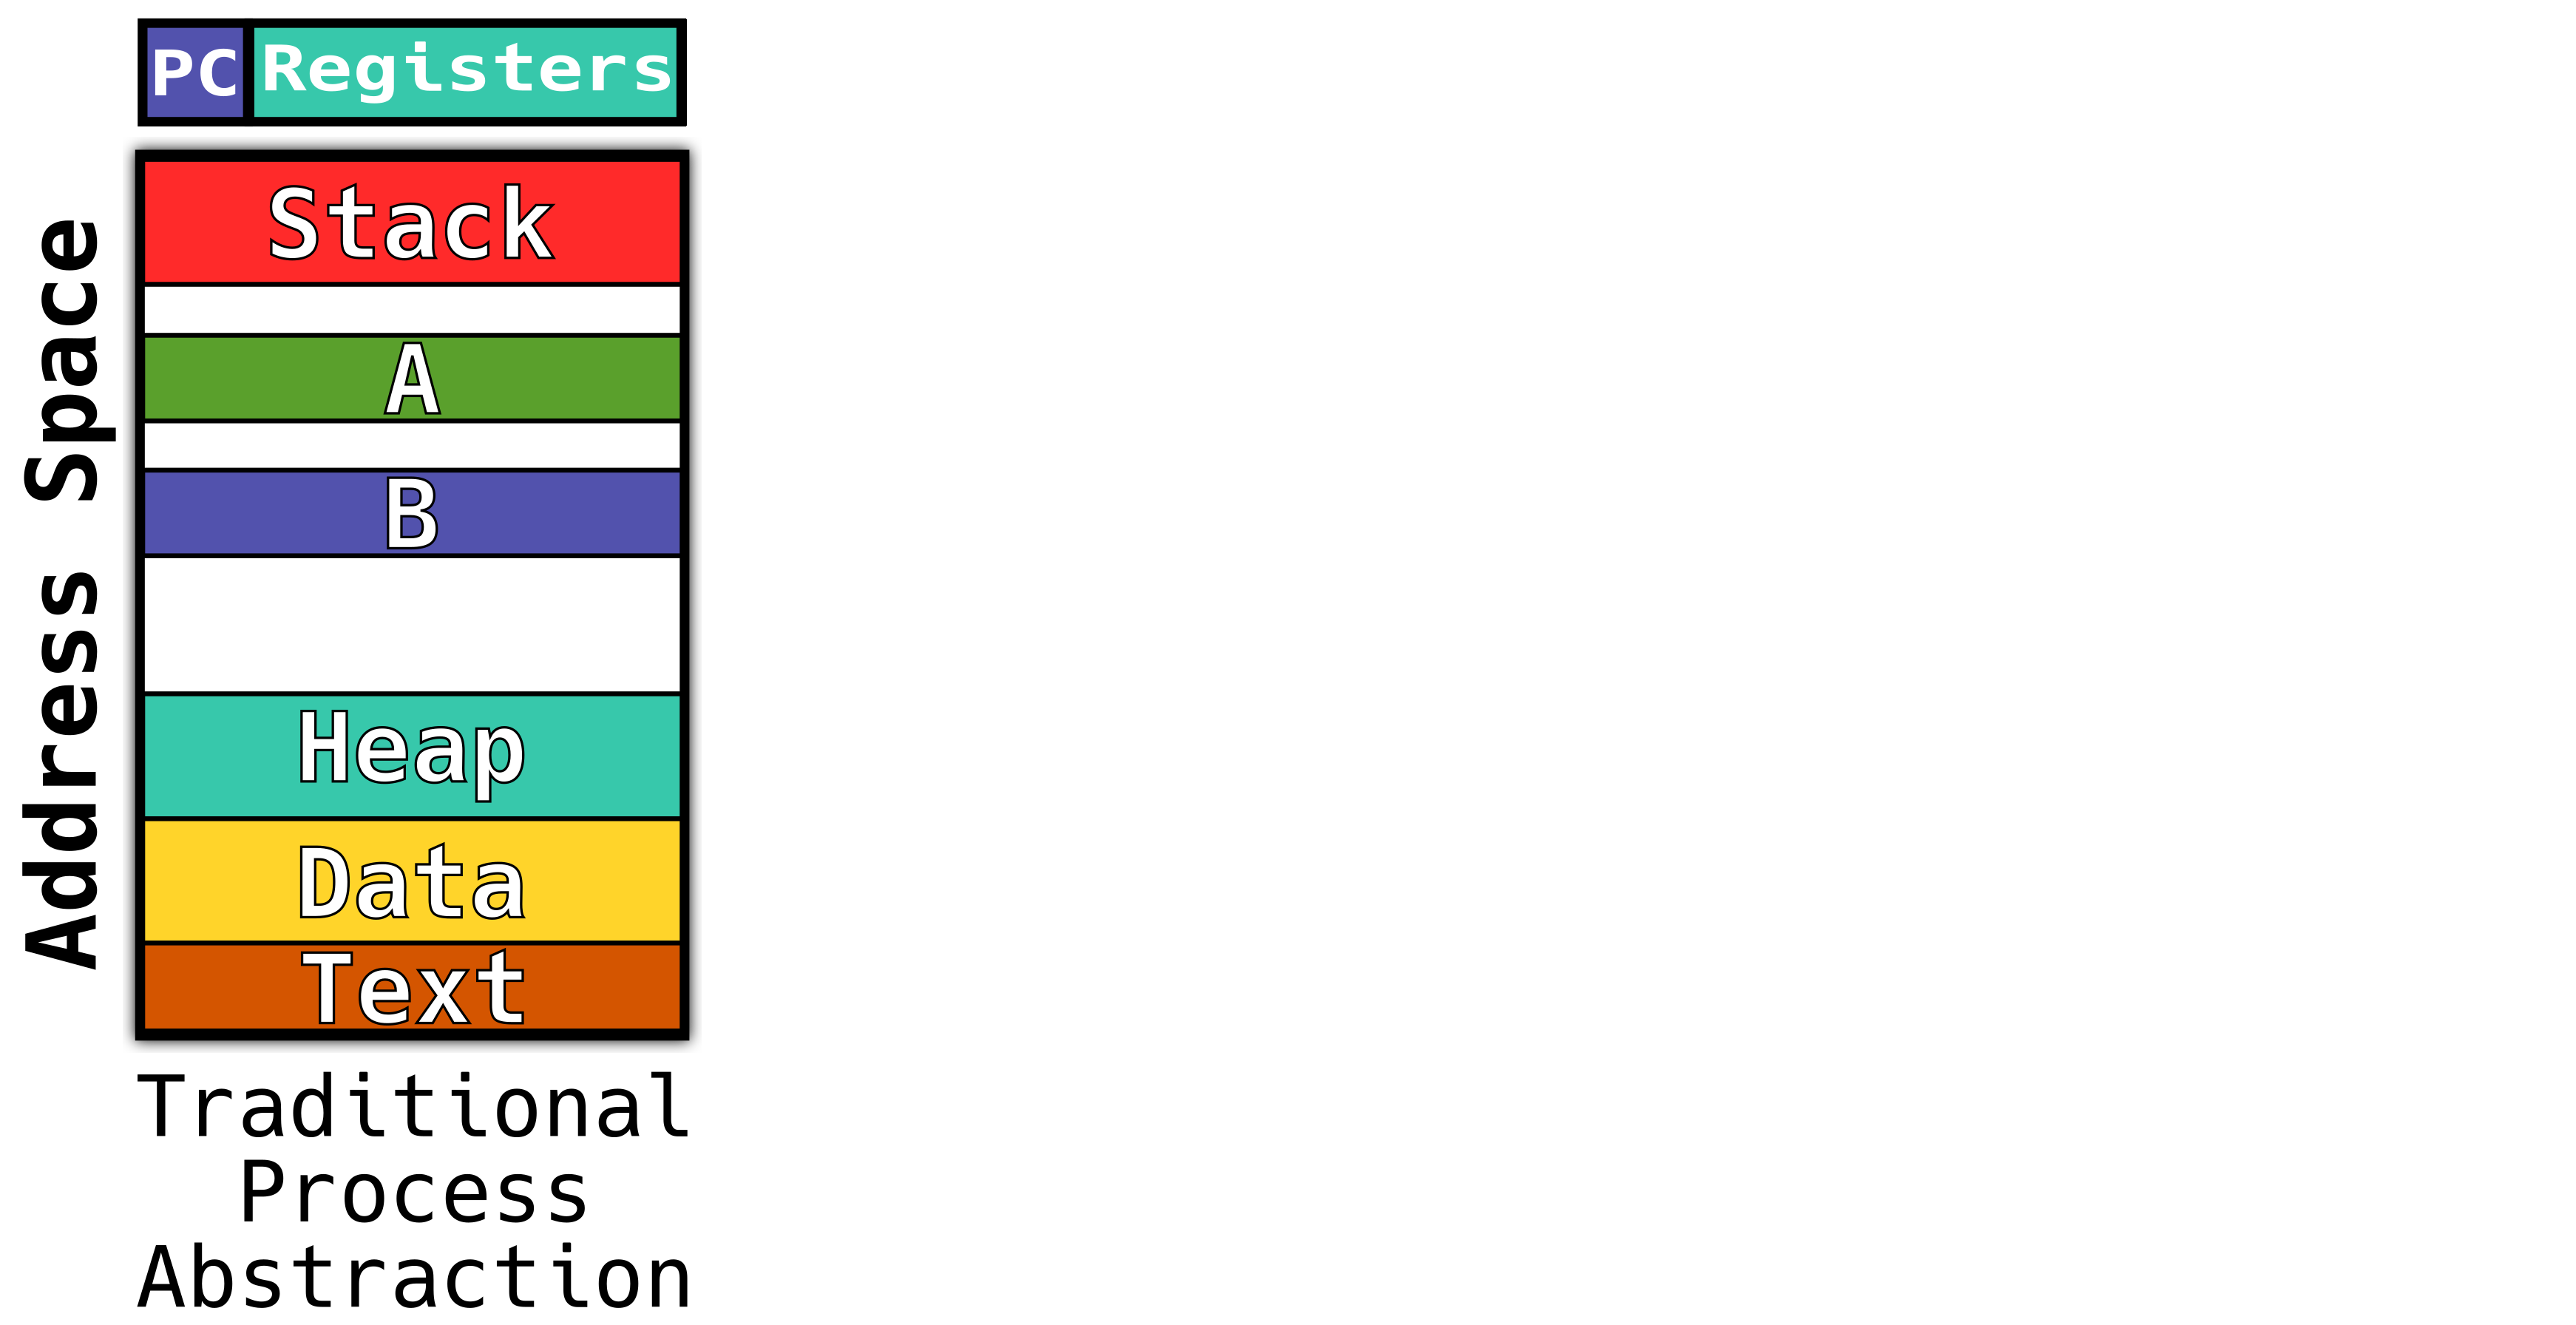
\includegraphics[width=0.7\textwidth, keepaspectratio=true]{images/traditional_vs_new_a.png}
  \end{figure}
\end{frame}

\begin{frame}{Design}{Multiple Virtual Address Space}
  \begin{figure}[ht]
    \centering
    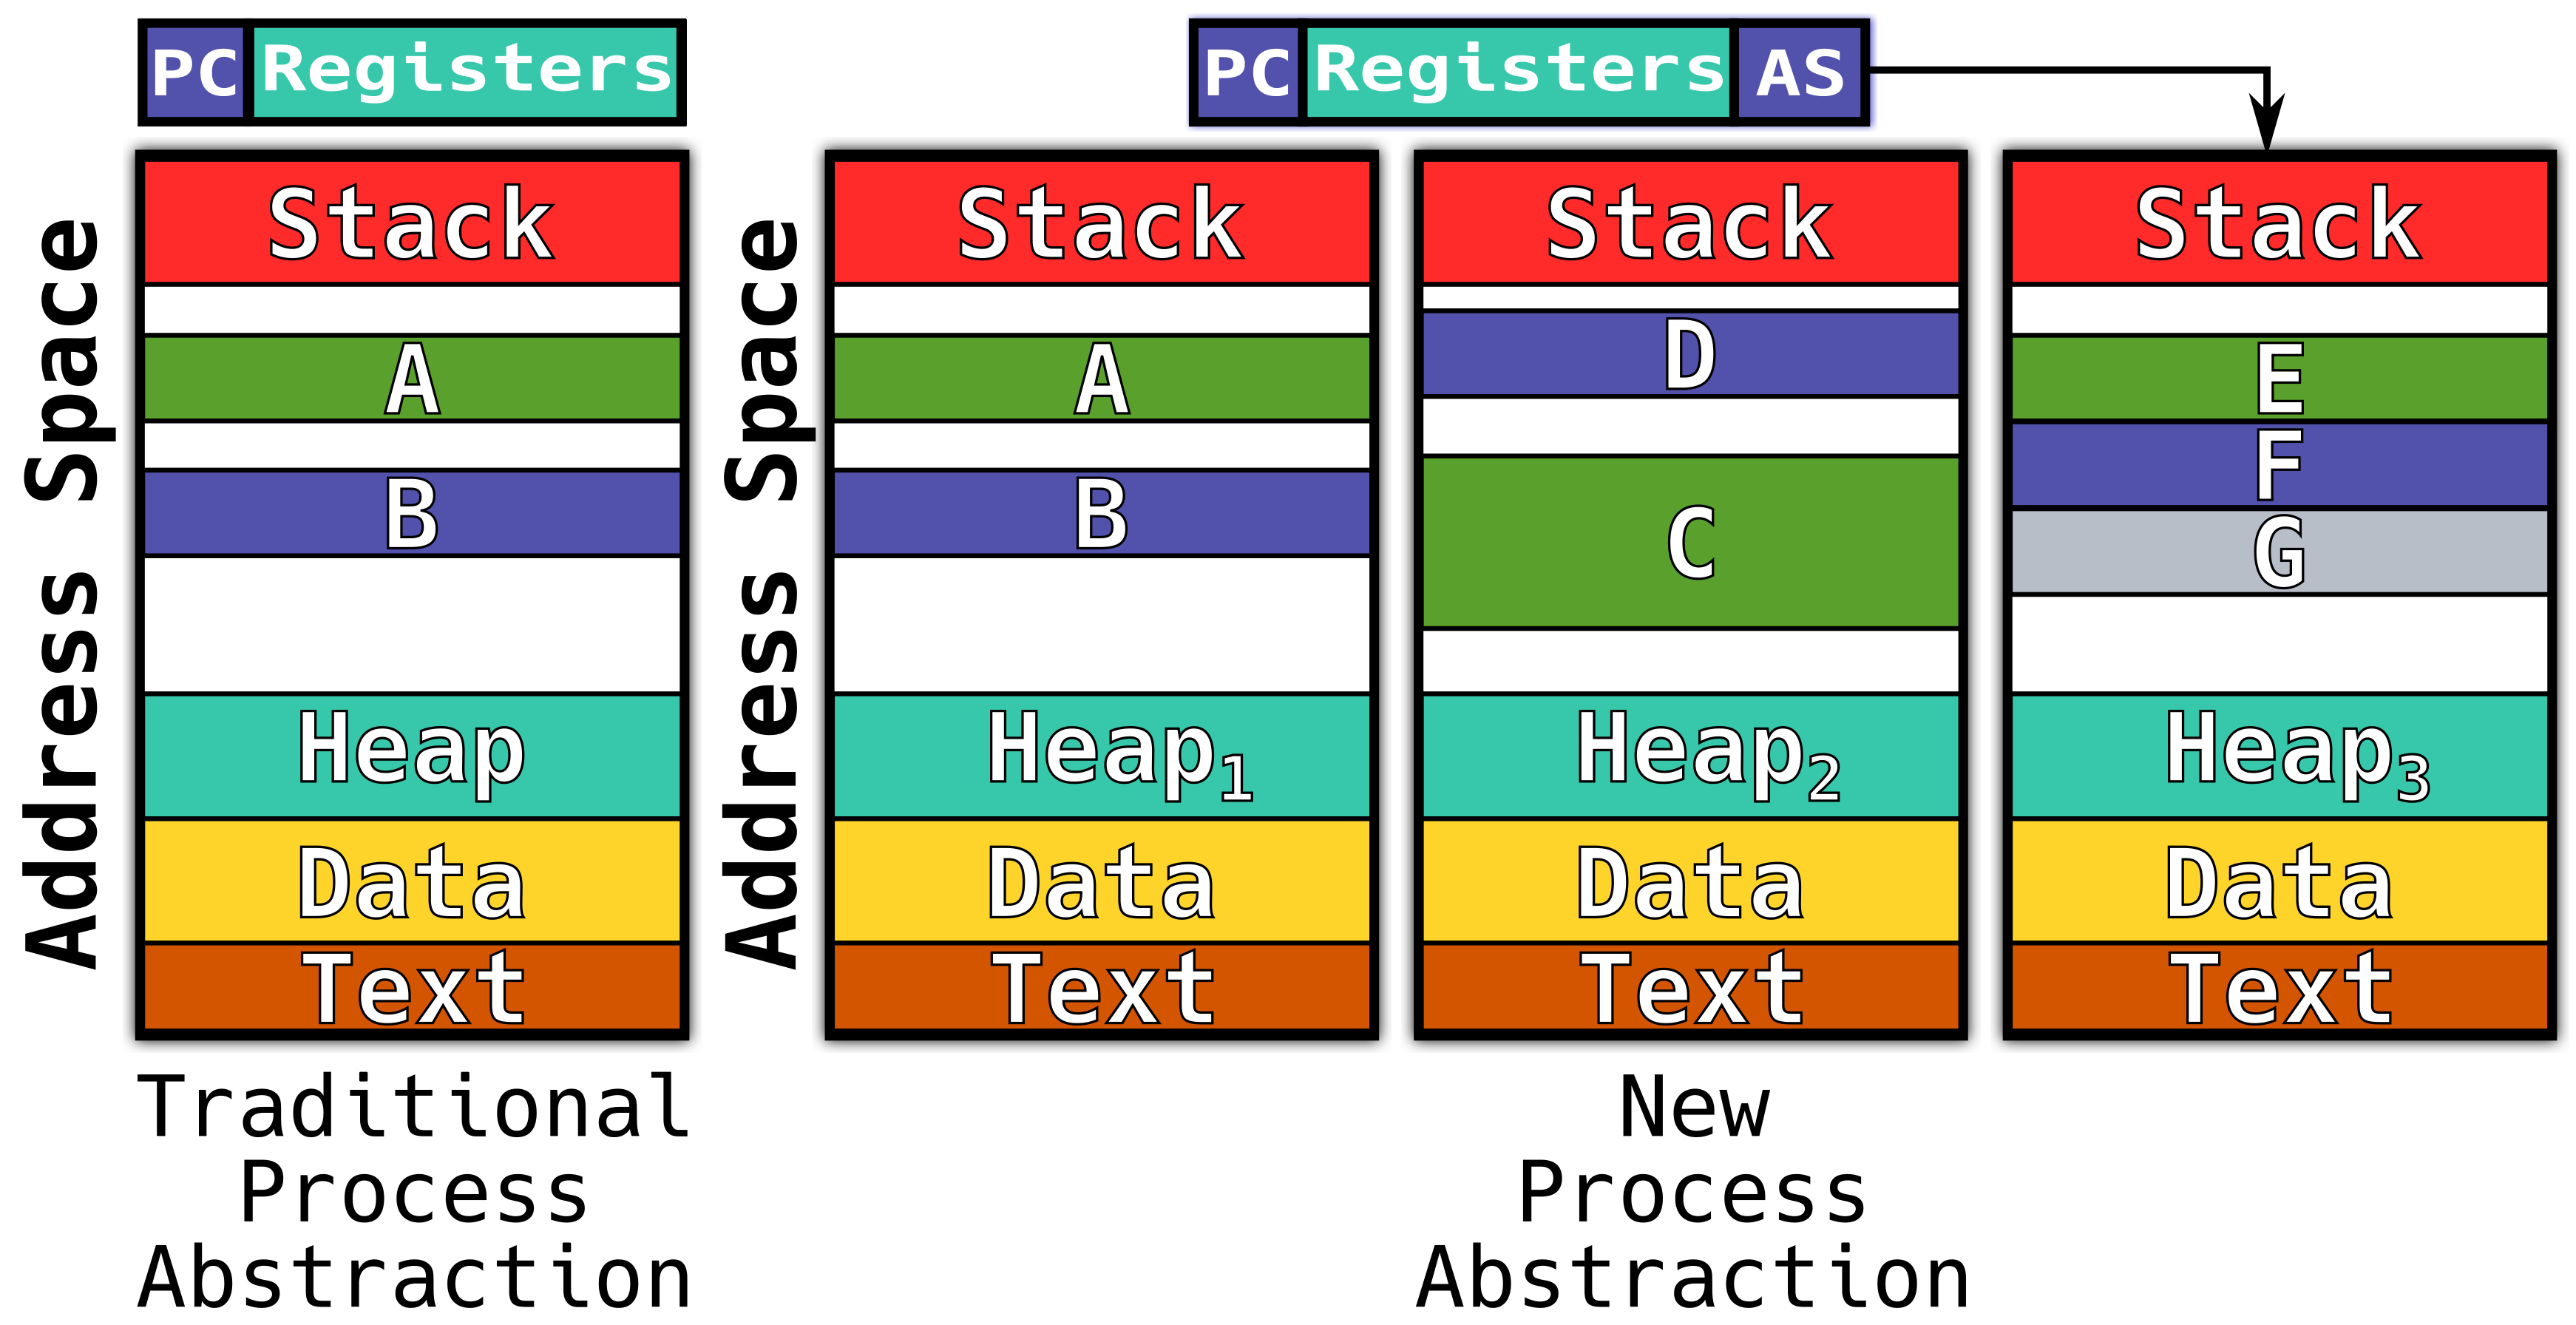
\includegraphics[width=0.7\textwidth, keepaspectratio=true]{images/traditional_vs_new_b.png}
  \end{figure}
\end{frame}

\begin{frame}[fragile]{Design}{SpaceJMP interface}
  \textbf{VAS API - for applications}
\begin{lstlisting}
vas_find(name) -> vid
vas_detach(vh)
vas_create(name, perms) -> vid
vas_clone(vid) -> vid
vas_attach(vid) -> vh
vas_switch(vh)
vas_ctl(cmd, vid[,arg])
\end{lstlisting}
\end{frame}

\begin{frame}[fragile]{Design}{SpaceJMP interface}
  \textbf{Segment API - for library developers}
\begin{lstlisting}
seg_find(name) -> sid
seg_attach(vh, sid)
seg_detach(vh, sid)
seg_ctl(sid, cmd[,arg])
seg_attach(vid, sid)
seg_detach(vid, sid)
seg_clone(sid) -> sid
seg_alloc(name, base, size, perms) -> sid
\end{lstlisting}
\end{frame}

\begin{frame}[fragile]{Design}{SpaceJMP interface}
  \textbf{Example: Using segment API}
\begin{lstlisting}
va = 0xC0DE;
sz = (1UL << 35);
vid = vas_create("v0", 660);
sid = seg_alloc("s0", va, sz, 660);
seg_attach(vid, sid);
\end{lstlisting}
\end{frame}

\begin{frame}[fragile]{Design}{SpaceJMP interface}
  \textbf{Example: Using API}
\begin{lstlisting}
vid = vas_find("v0");
vh = vas_attach(vid);
vas_switch(vh);
t = malloc(...);
*t = 42;
\end{lstlisting}
\end{frame}

%-------------------------------------------------------
% Example
%-------------------------------------------------------
\section{Example}
\begin{frame}{Example}{Example}
  \begin{figure}[ht]
    \centering
    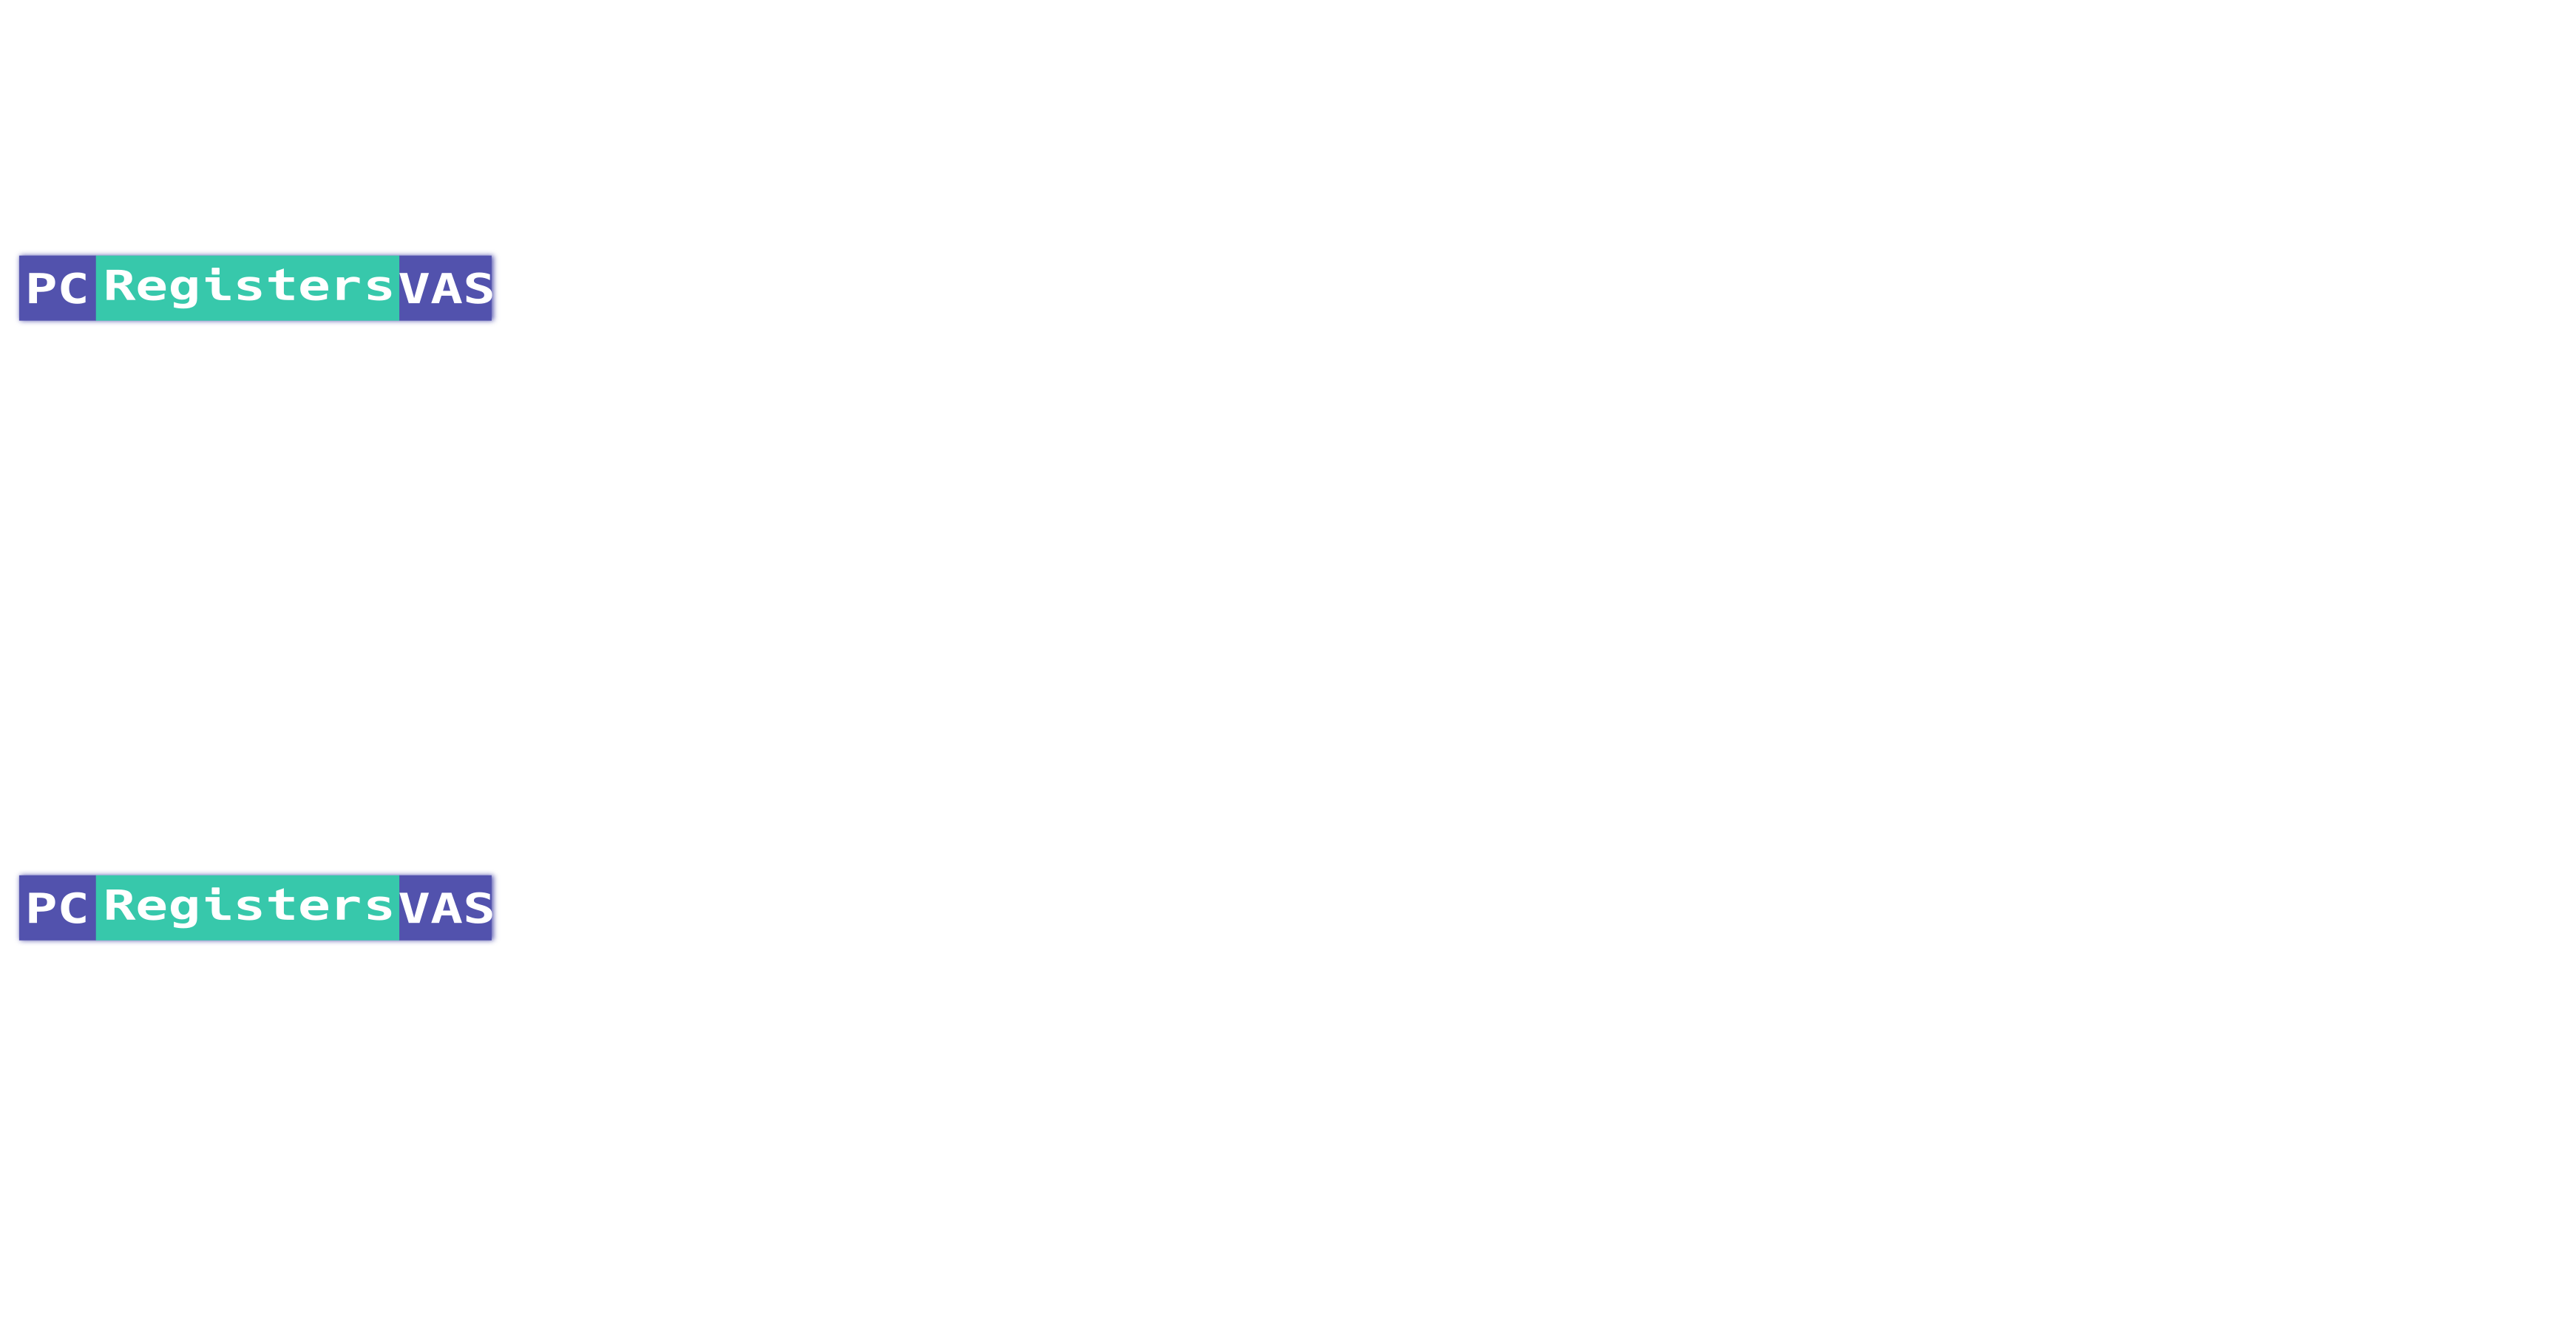
\includegraphics[width=1\textwidth, keepaspectratio=true]{images/spacejmp_example_a.png}
  \end{figure}
\end{frame}

\begin{frame}{Example}{Example}
  \begin{figure}[ht]
    \centering
    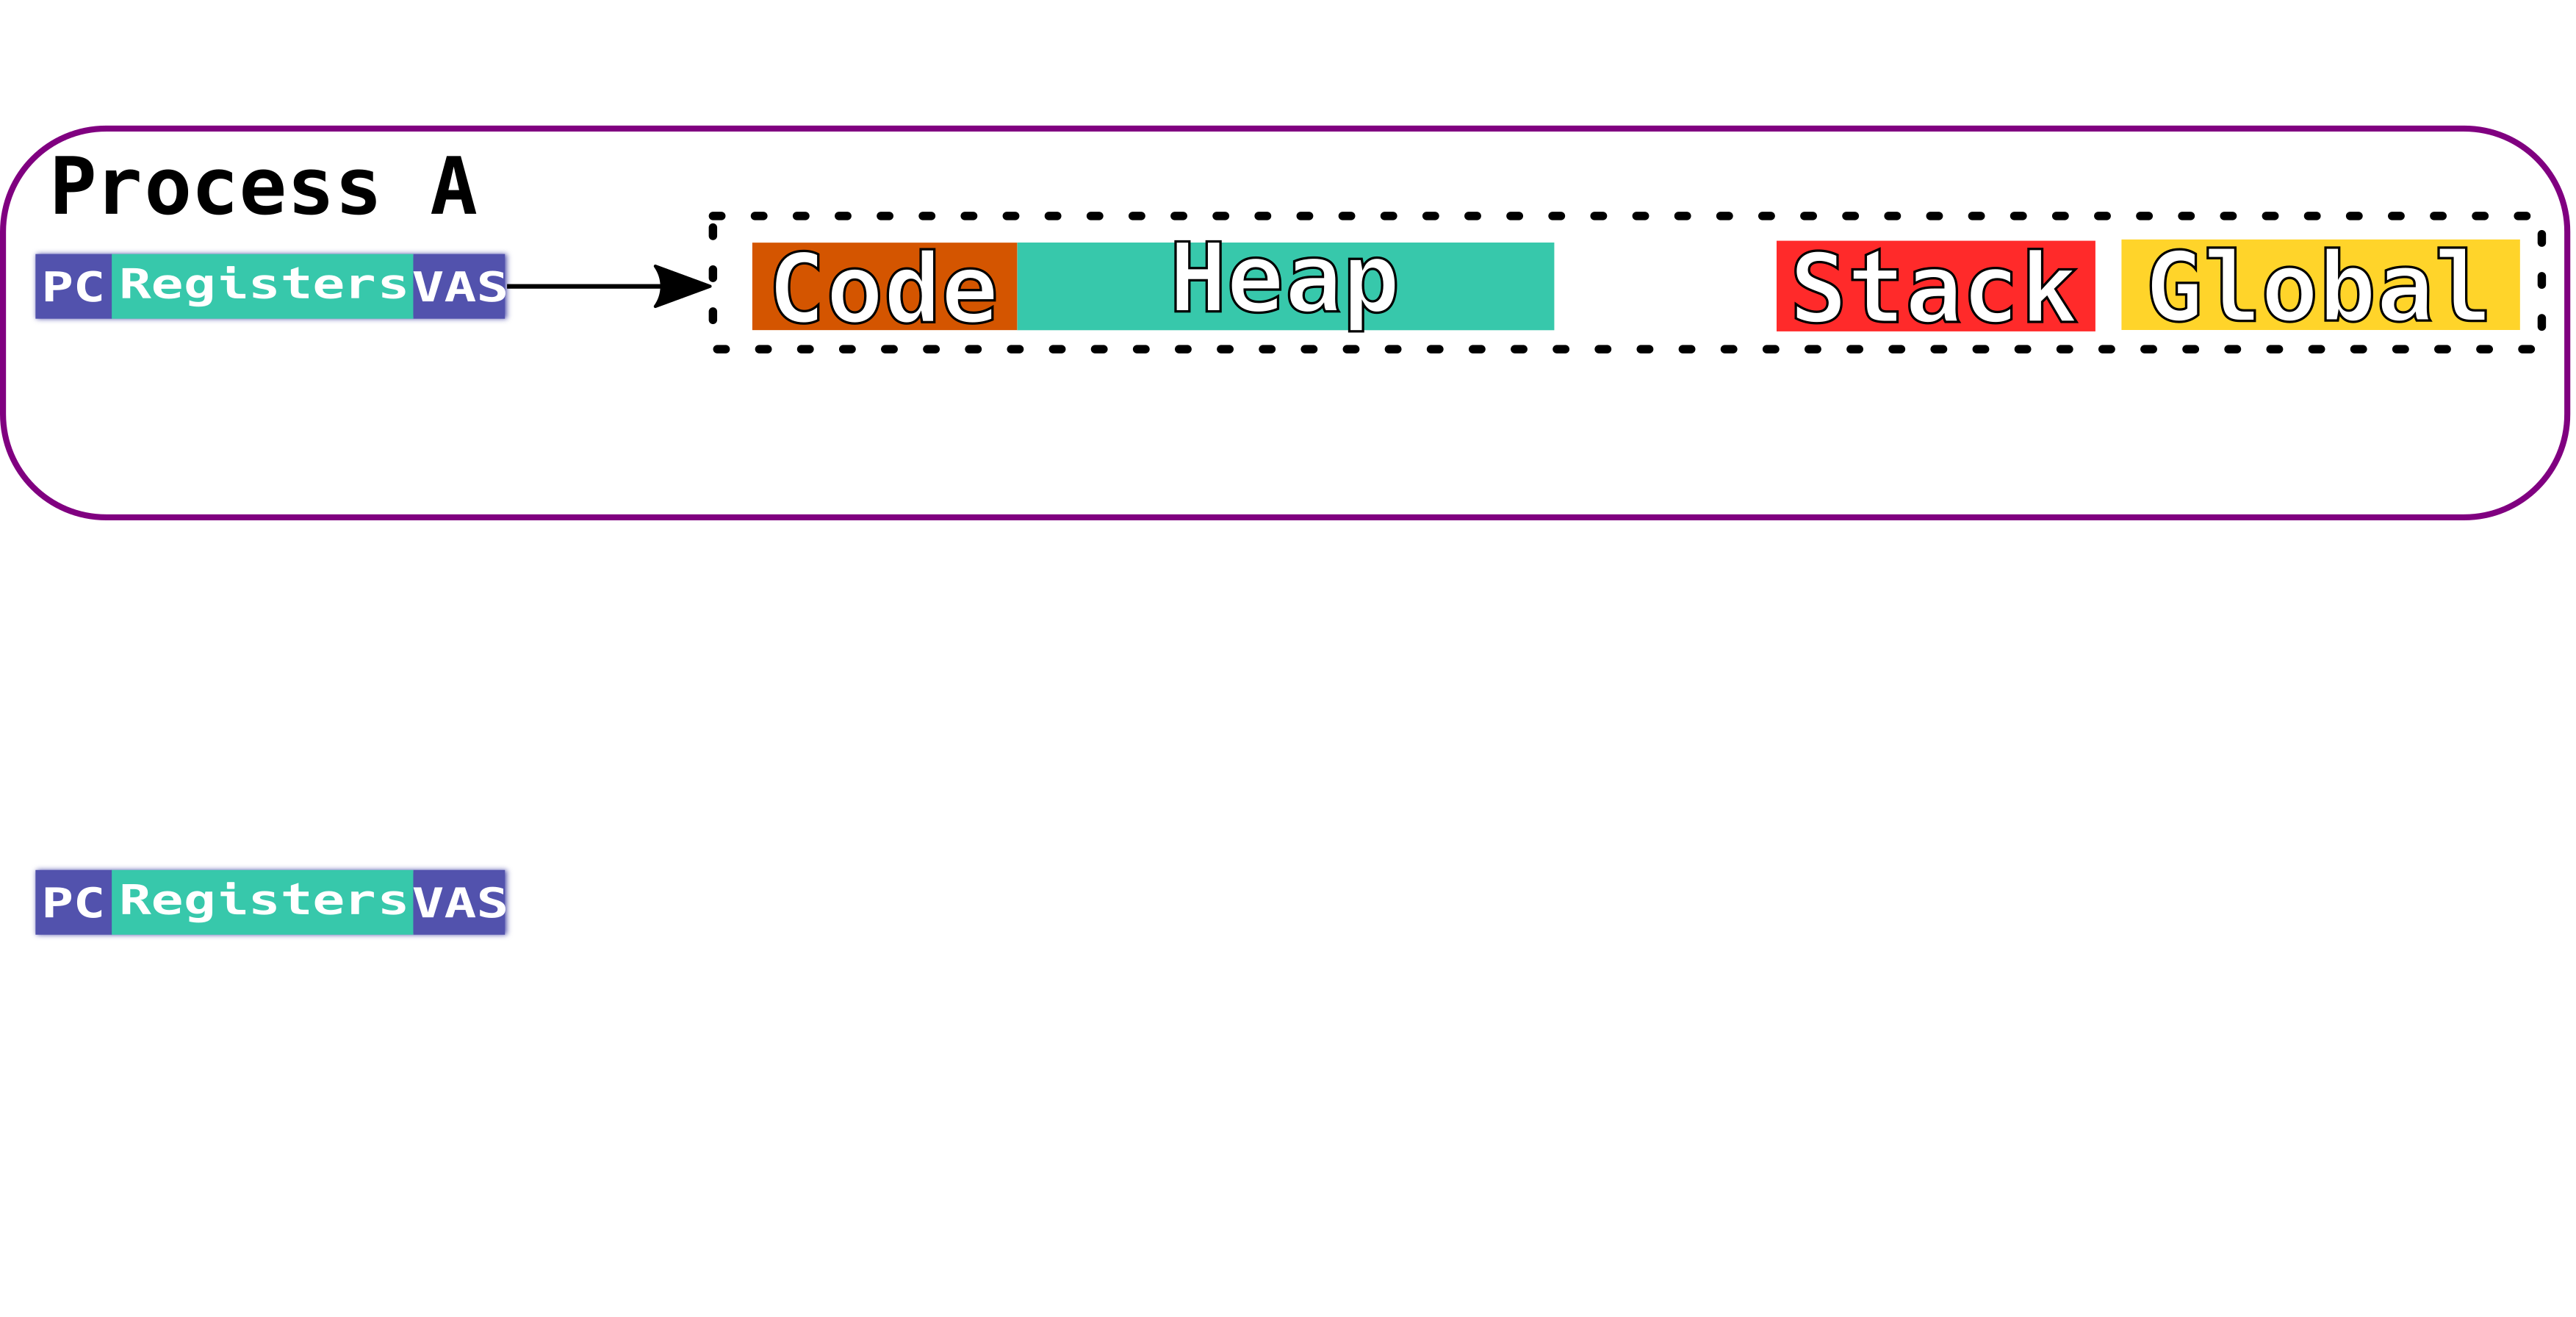
\includegraphics[width=1\textwidth, keepaspectratio=true]{images/spacejmp_example_b.png}
  \end{figure}
\end{frame}

\begin{frame}{Example}{Example}
  \begin{figure}[ht]
    \centering
    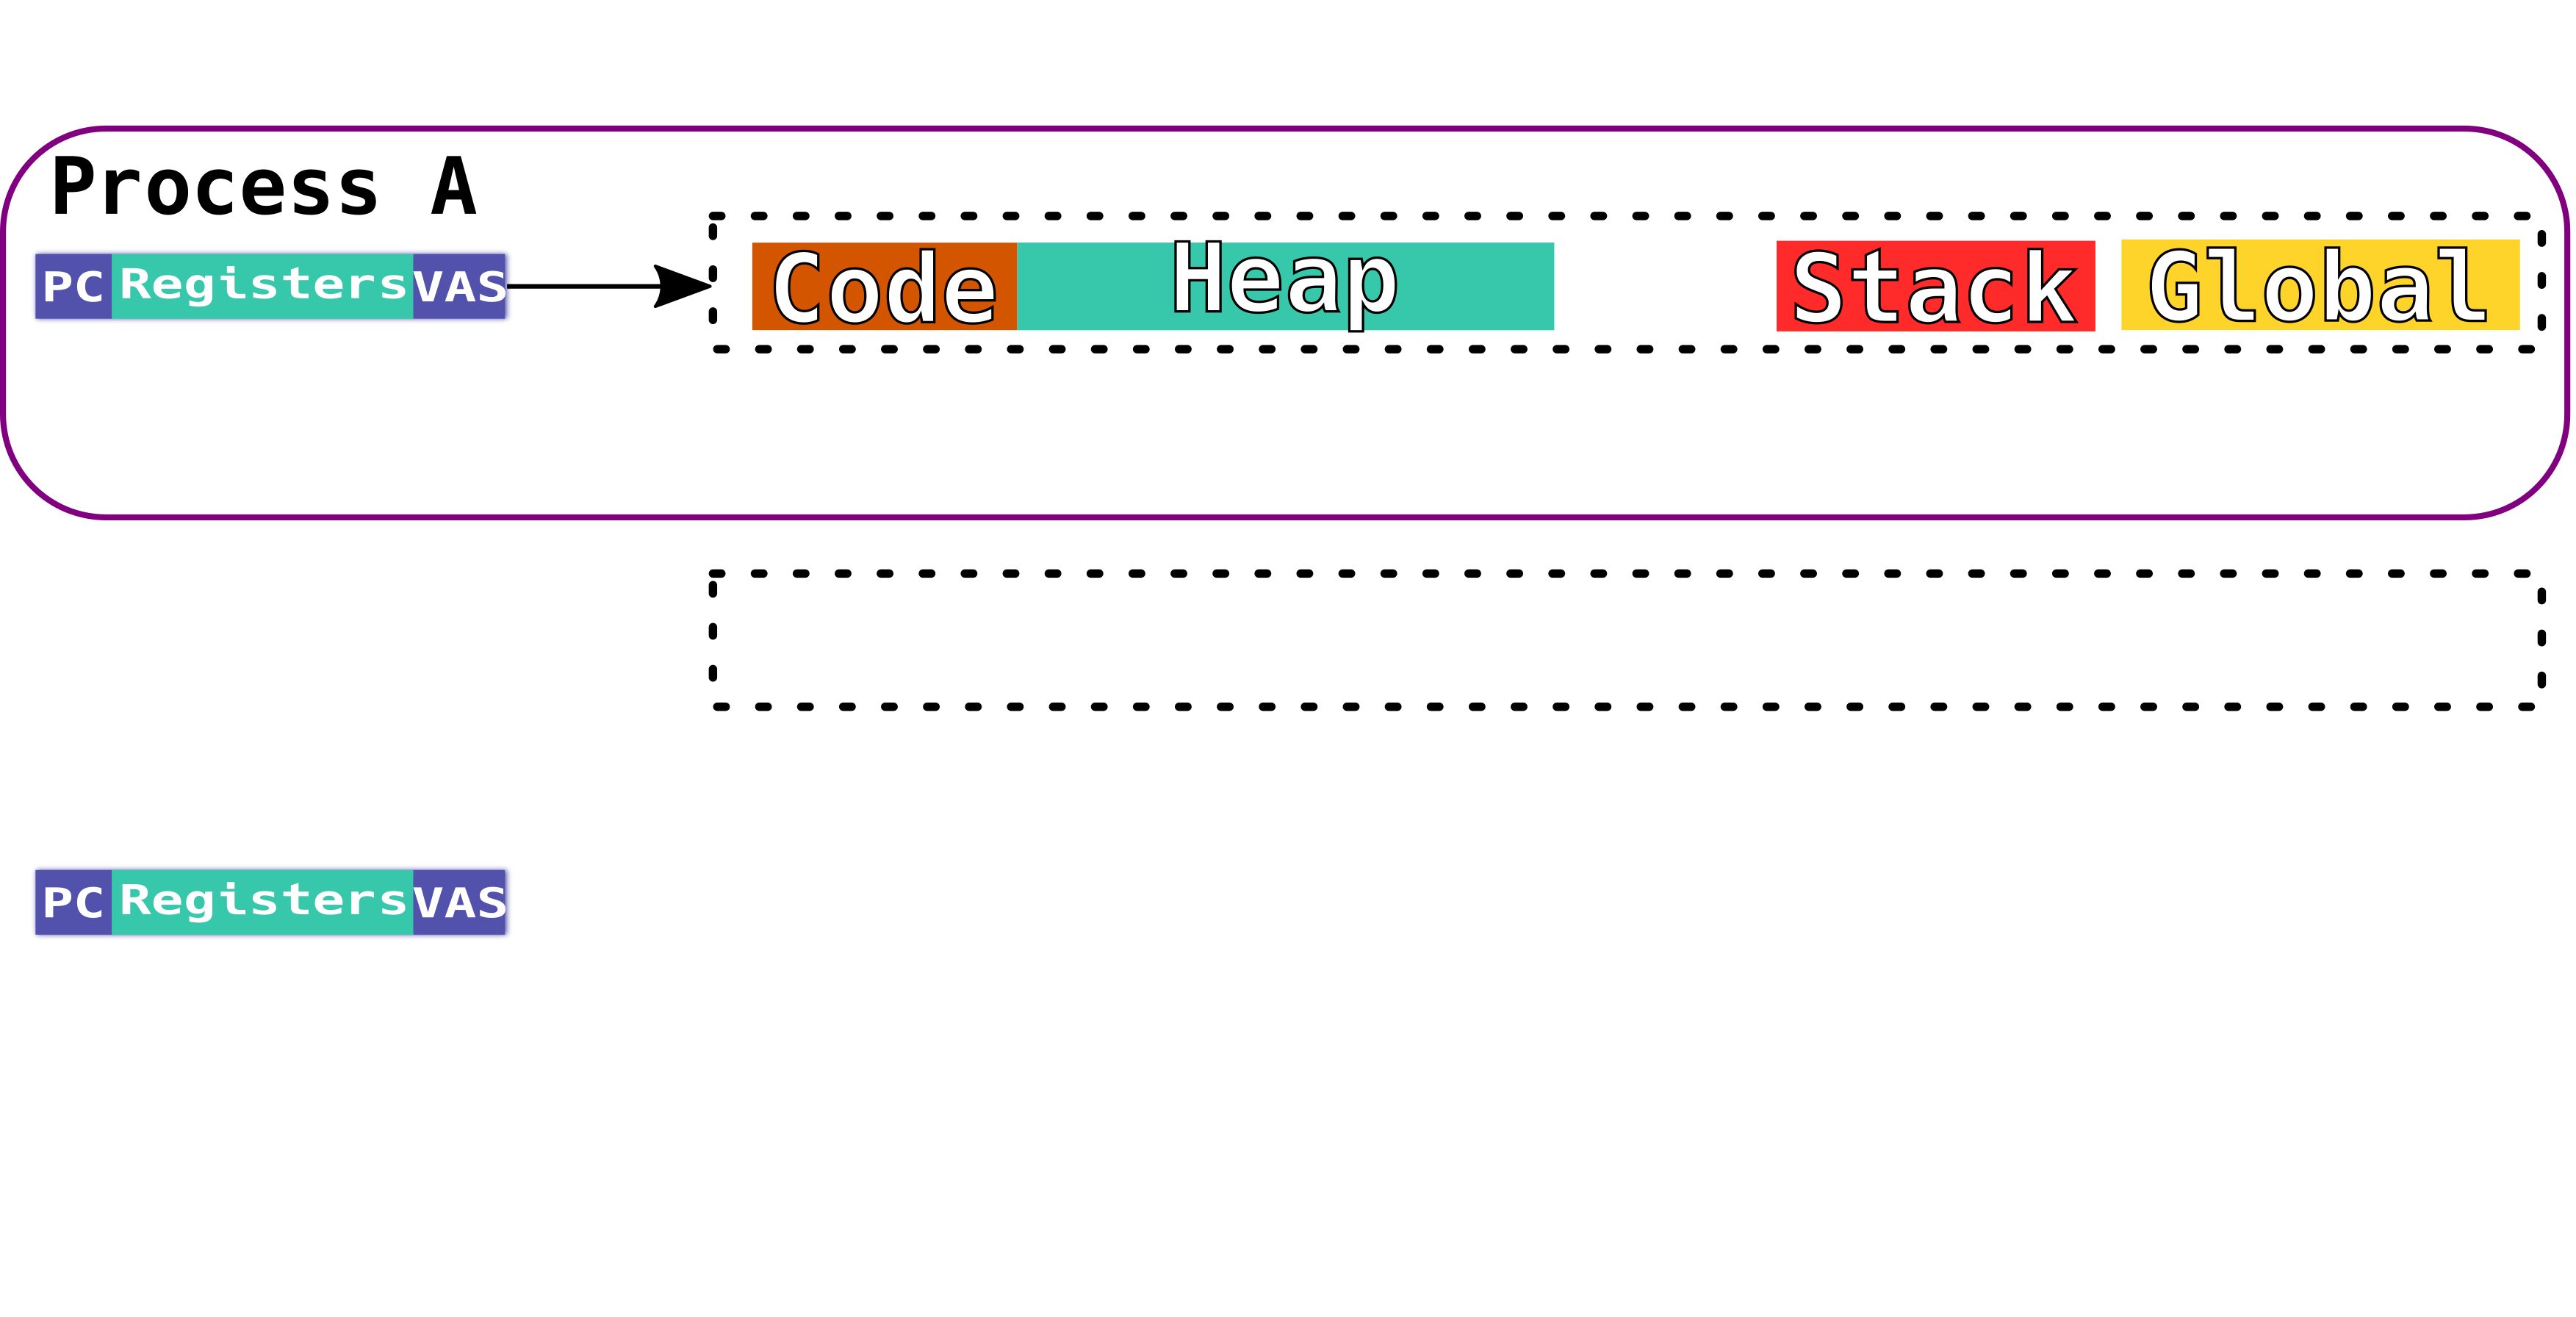
\includegraphics[width=1\textwidth, keepaspectratio=true]{images/spacejmp_example_c.png}
  \end{figure}
\end{frame}

\begin{frame}{Example}{Example}
  \begin{figure}[ht]
    \centering
    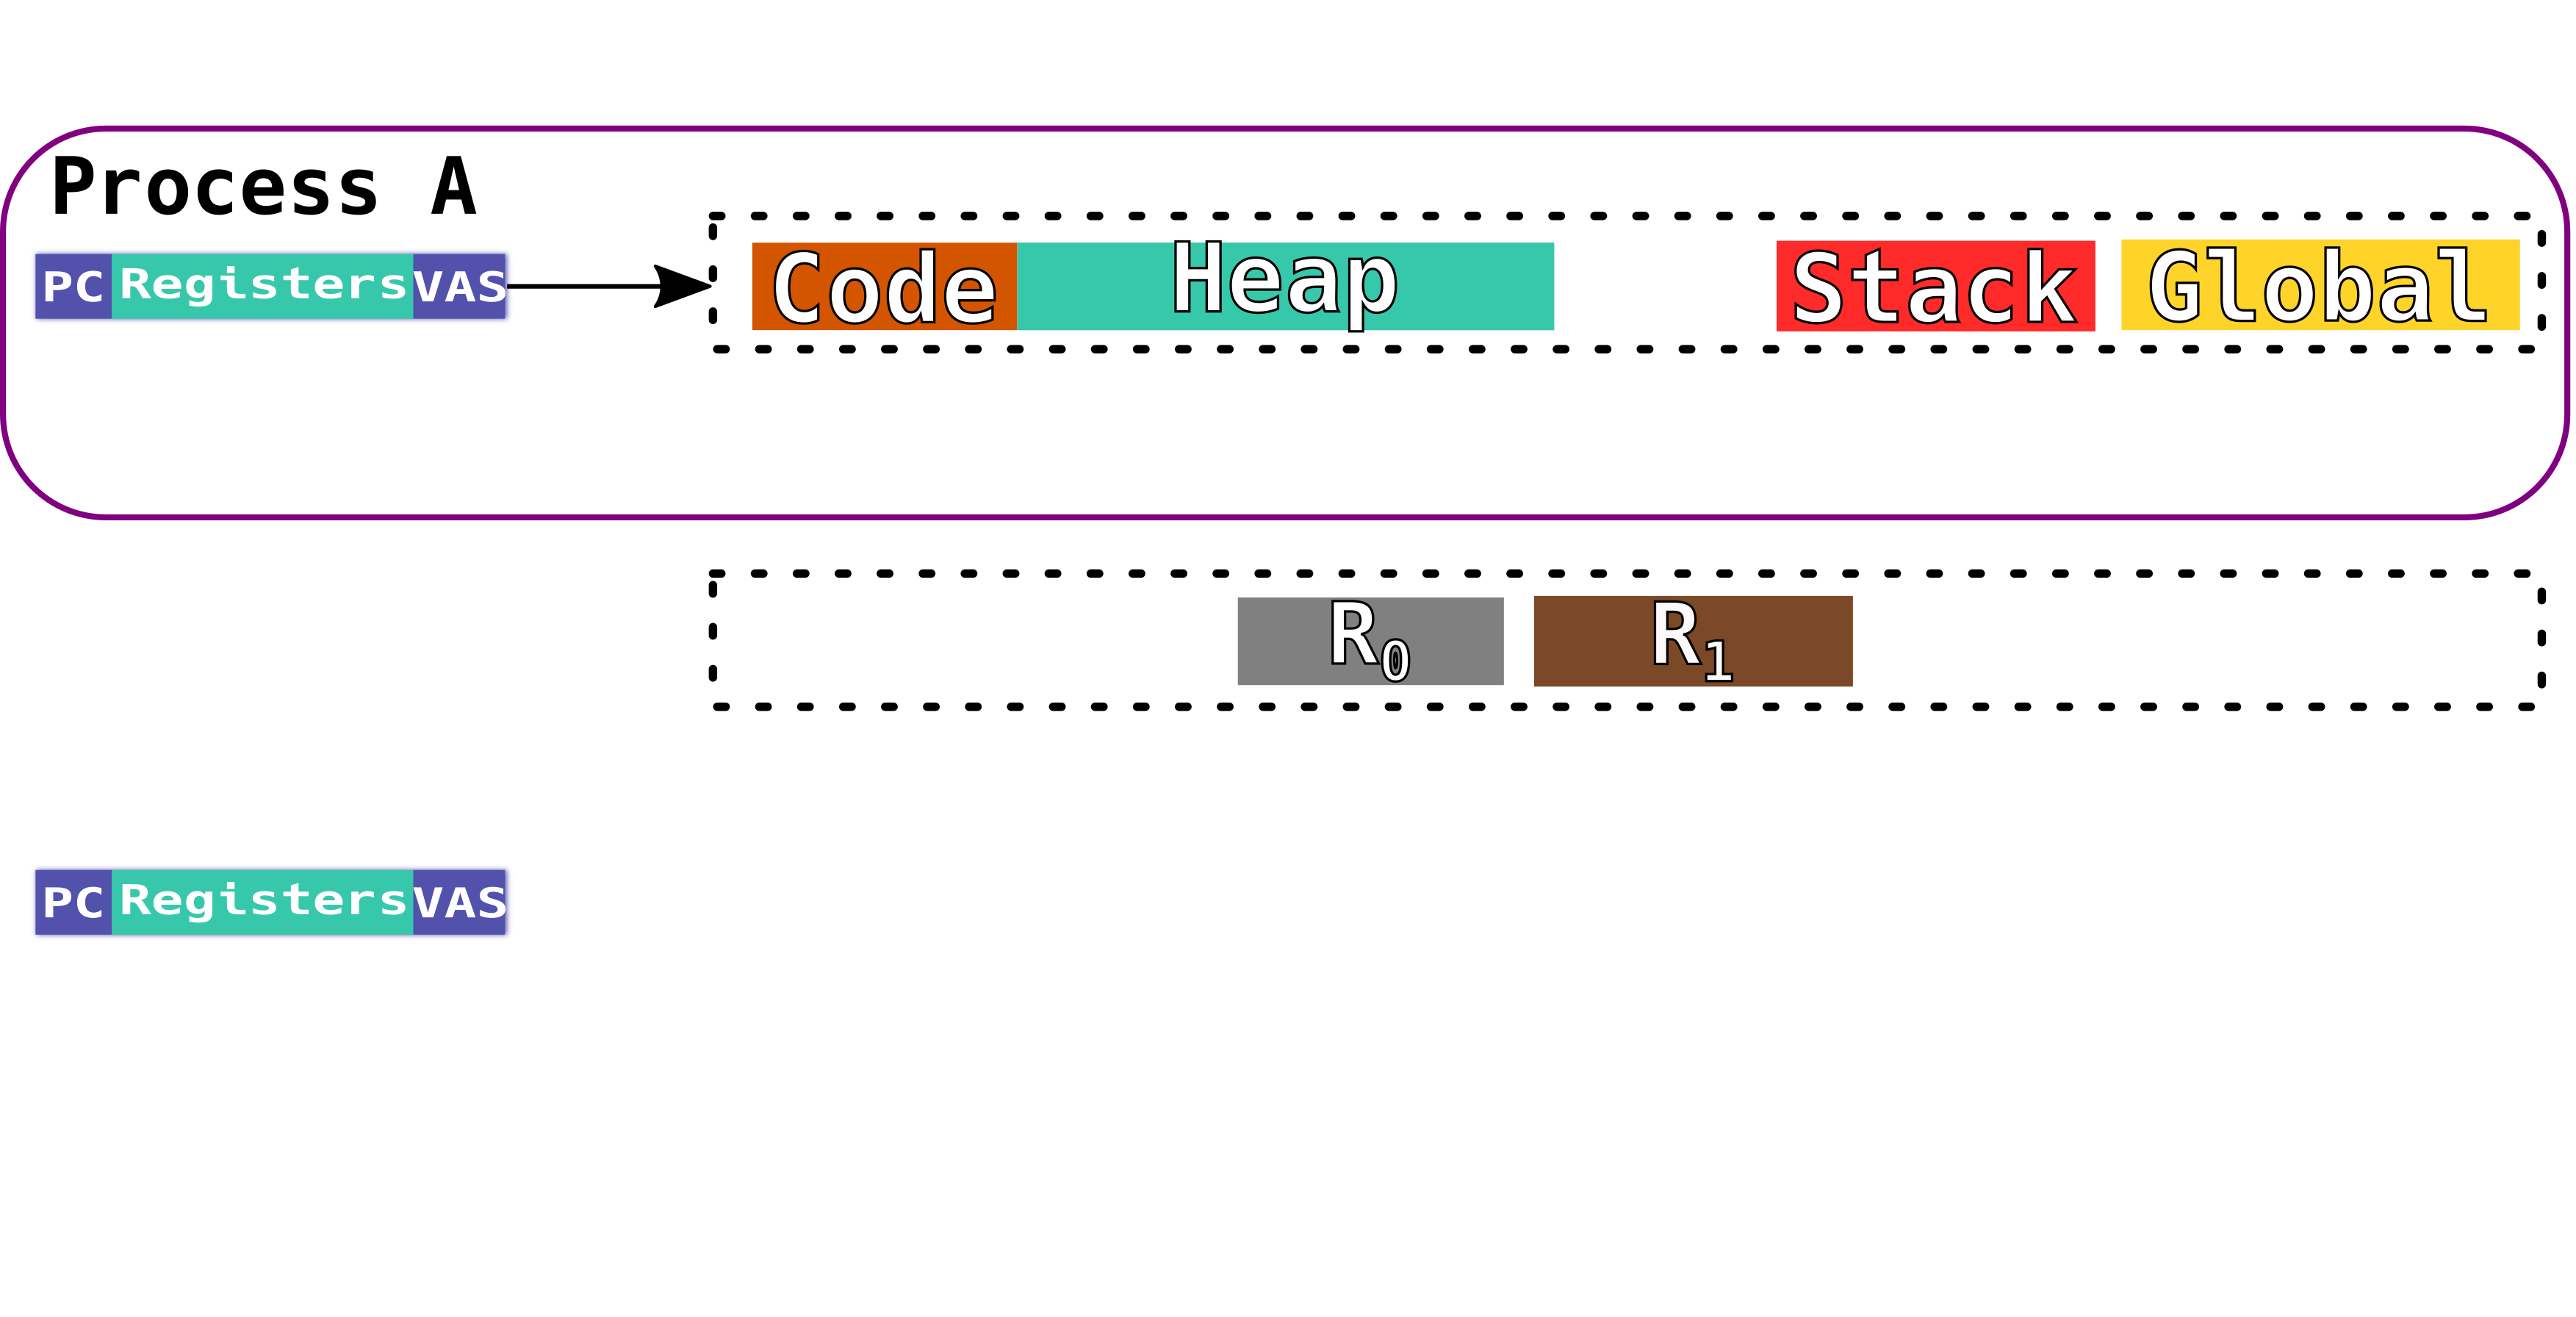
\includegraphics[width=1\textwidth, keepaspectratio=true]{images/spacejmp_example_d.png}
  \end{figure}
\end{frame}

\begin{frame}{Example}{Example}
  \begin{figure}[ht]
    \centering
    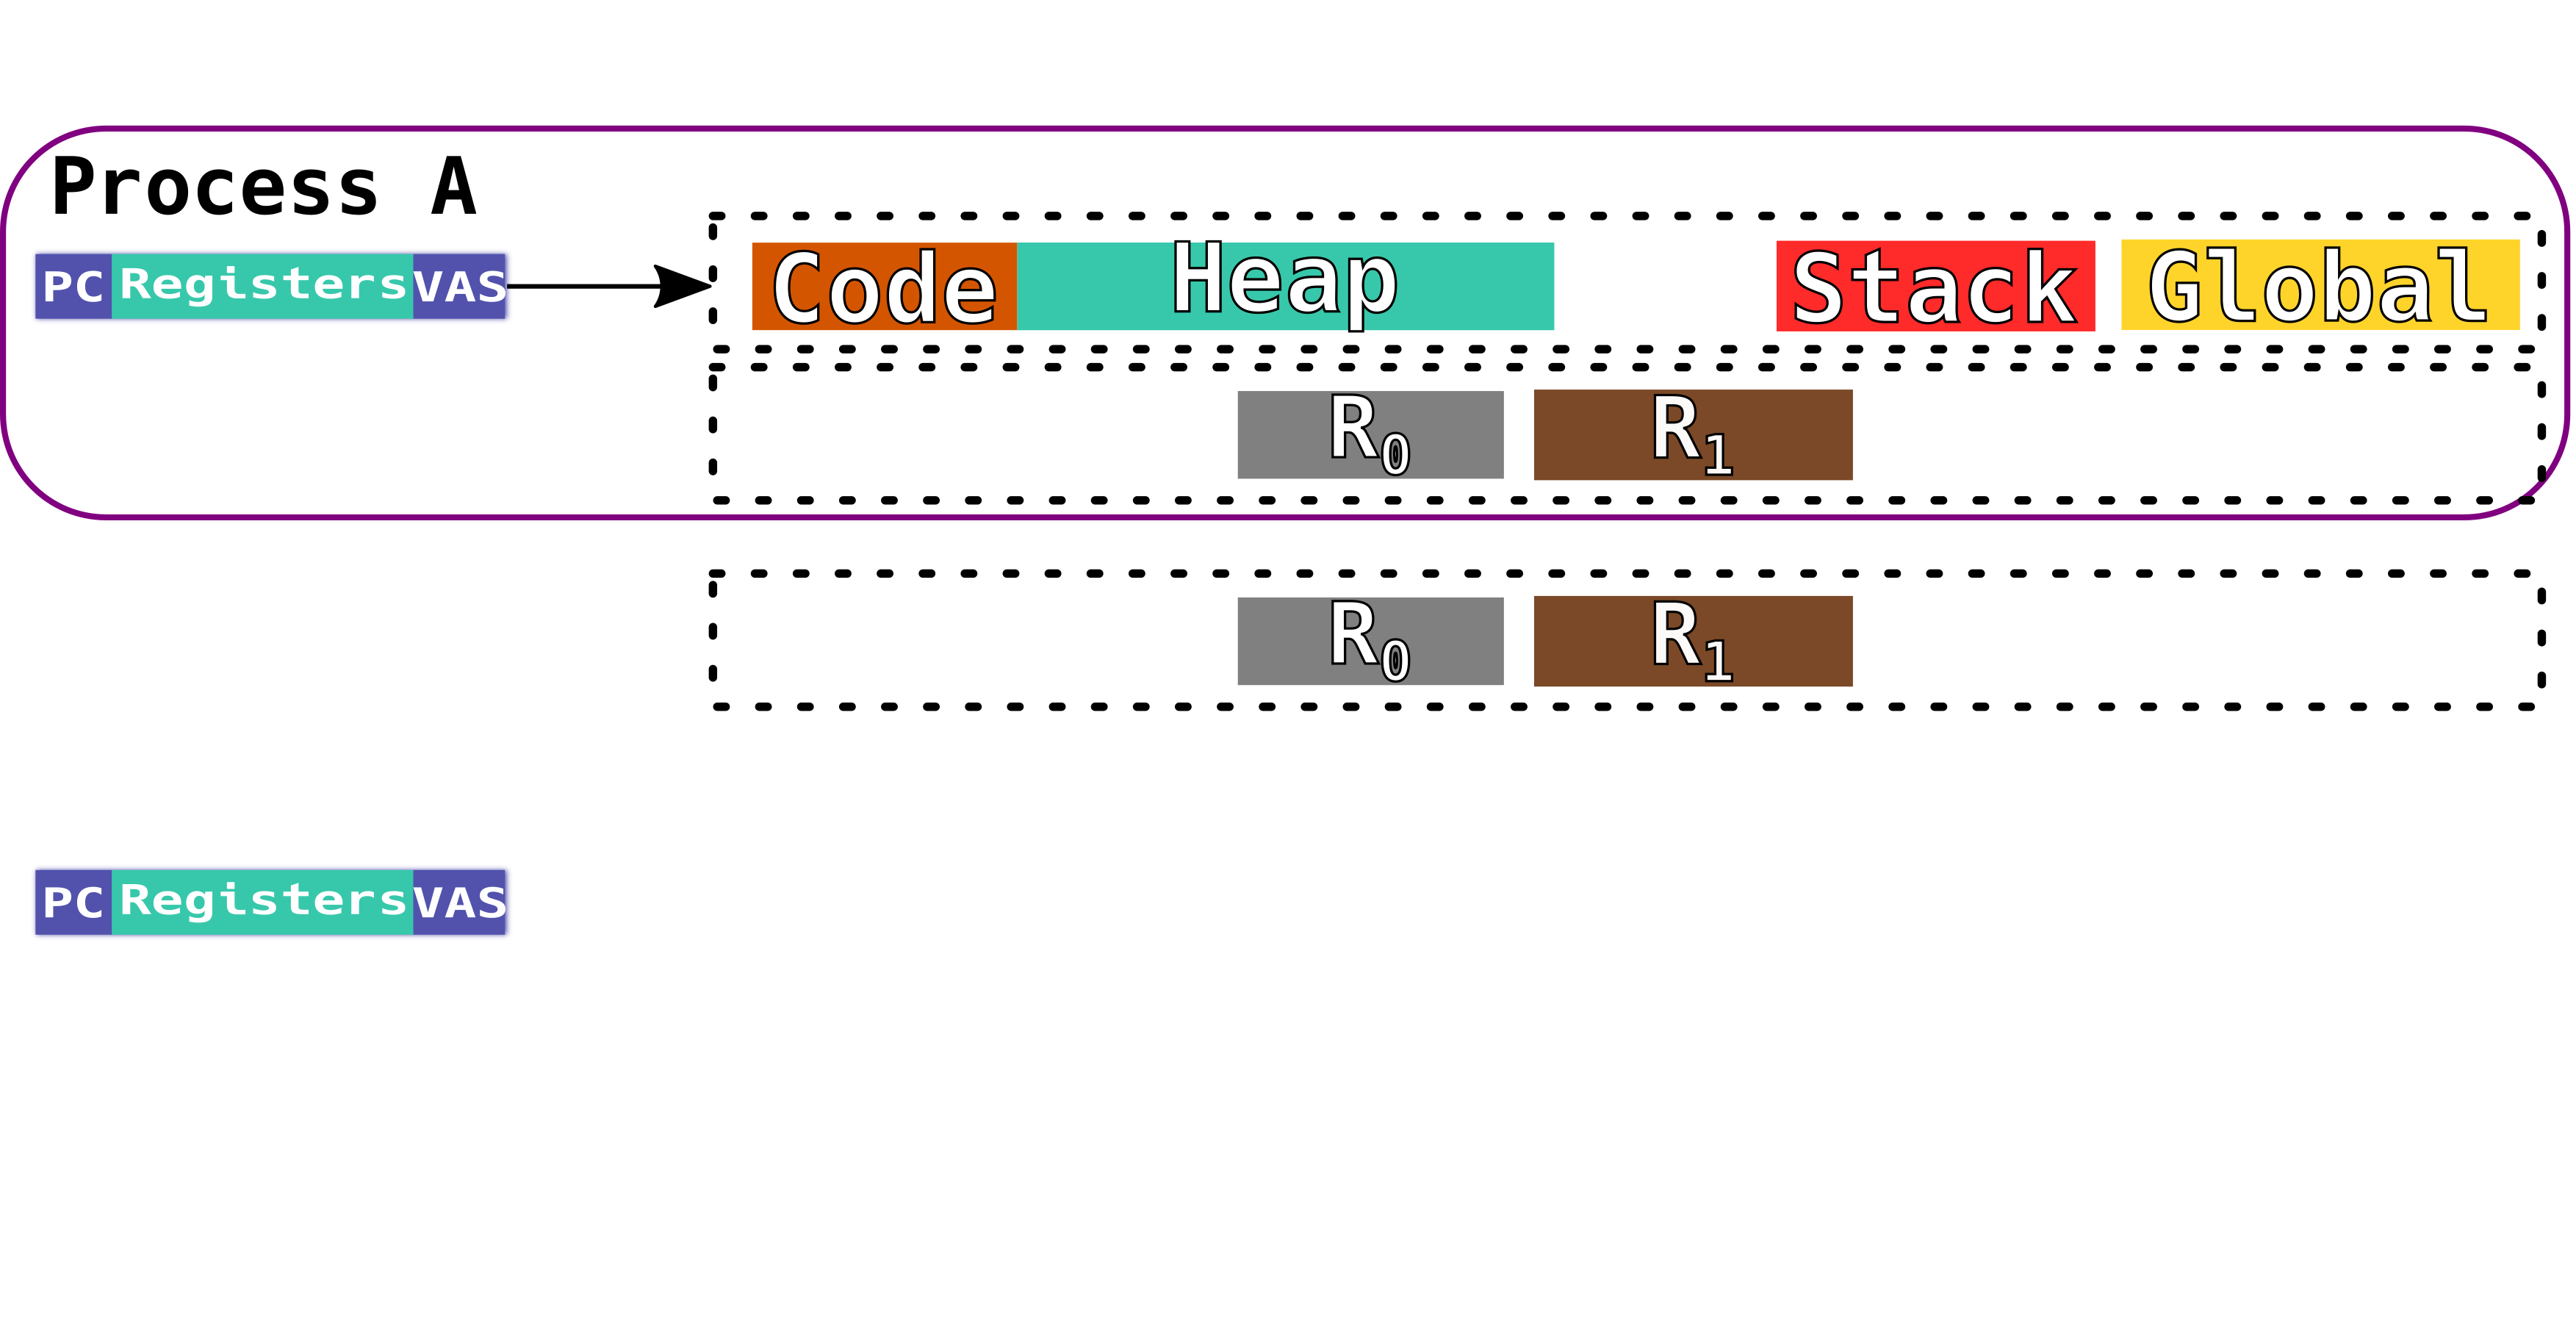
\includegraphics[width=1\textwidth, keepaspectratio=true]{images/spacejmp_example_e.png}
  \end{figure}
\end{frame}

\begin{frame}{Example}{Example}
  \begin{figure}[ht]
    \centering
    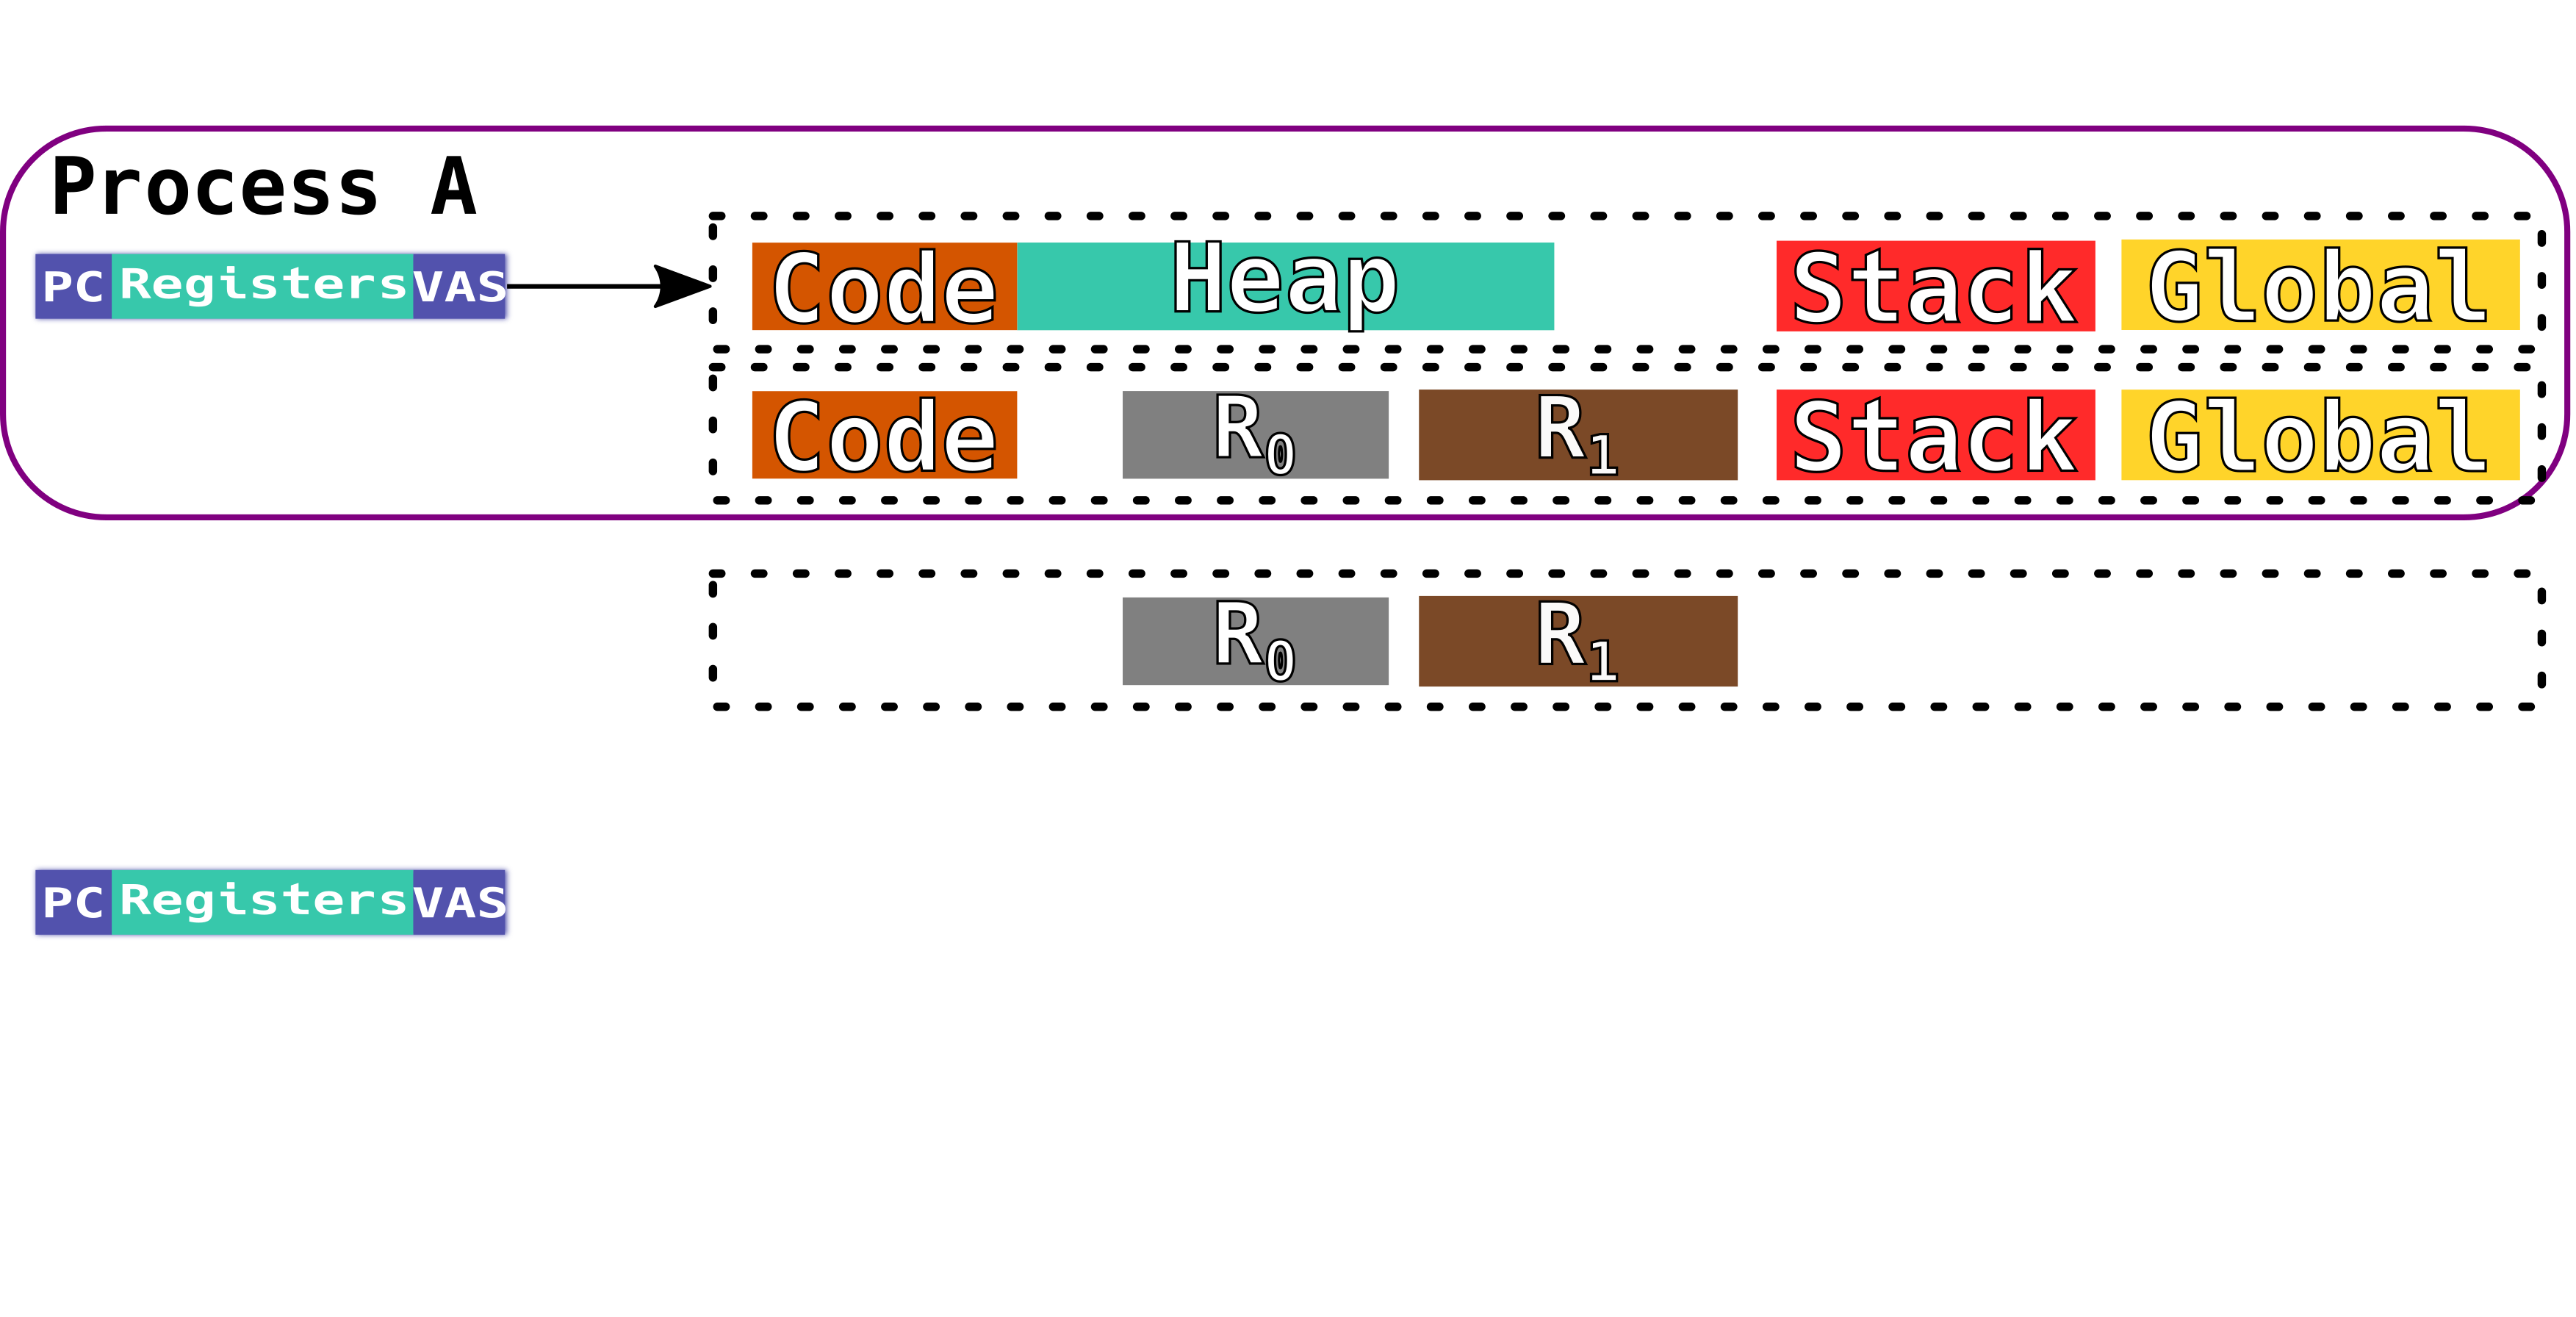
\includegraphics[width=1\textwidth, keepaspectratio=true]{images/spacejmp_example_f.png}
  \end{figure}
\end{frame}

\begin{frame}{Example}{Example}
  \begin{figure}[ht]
    \centering
    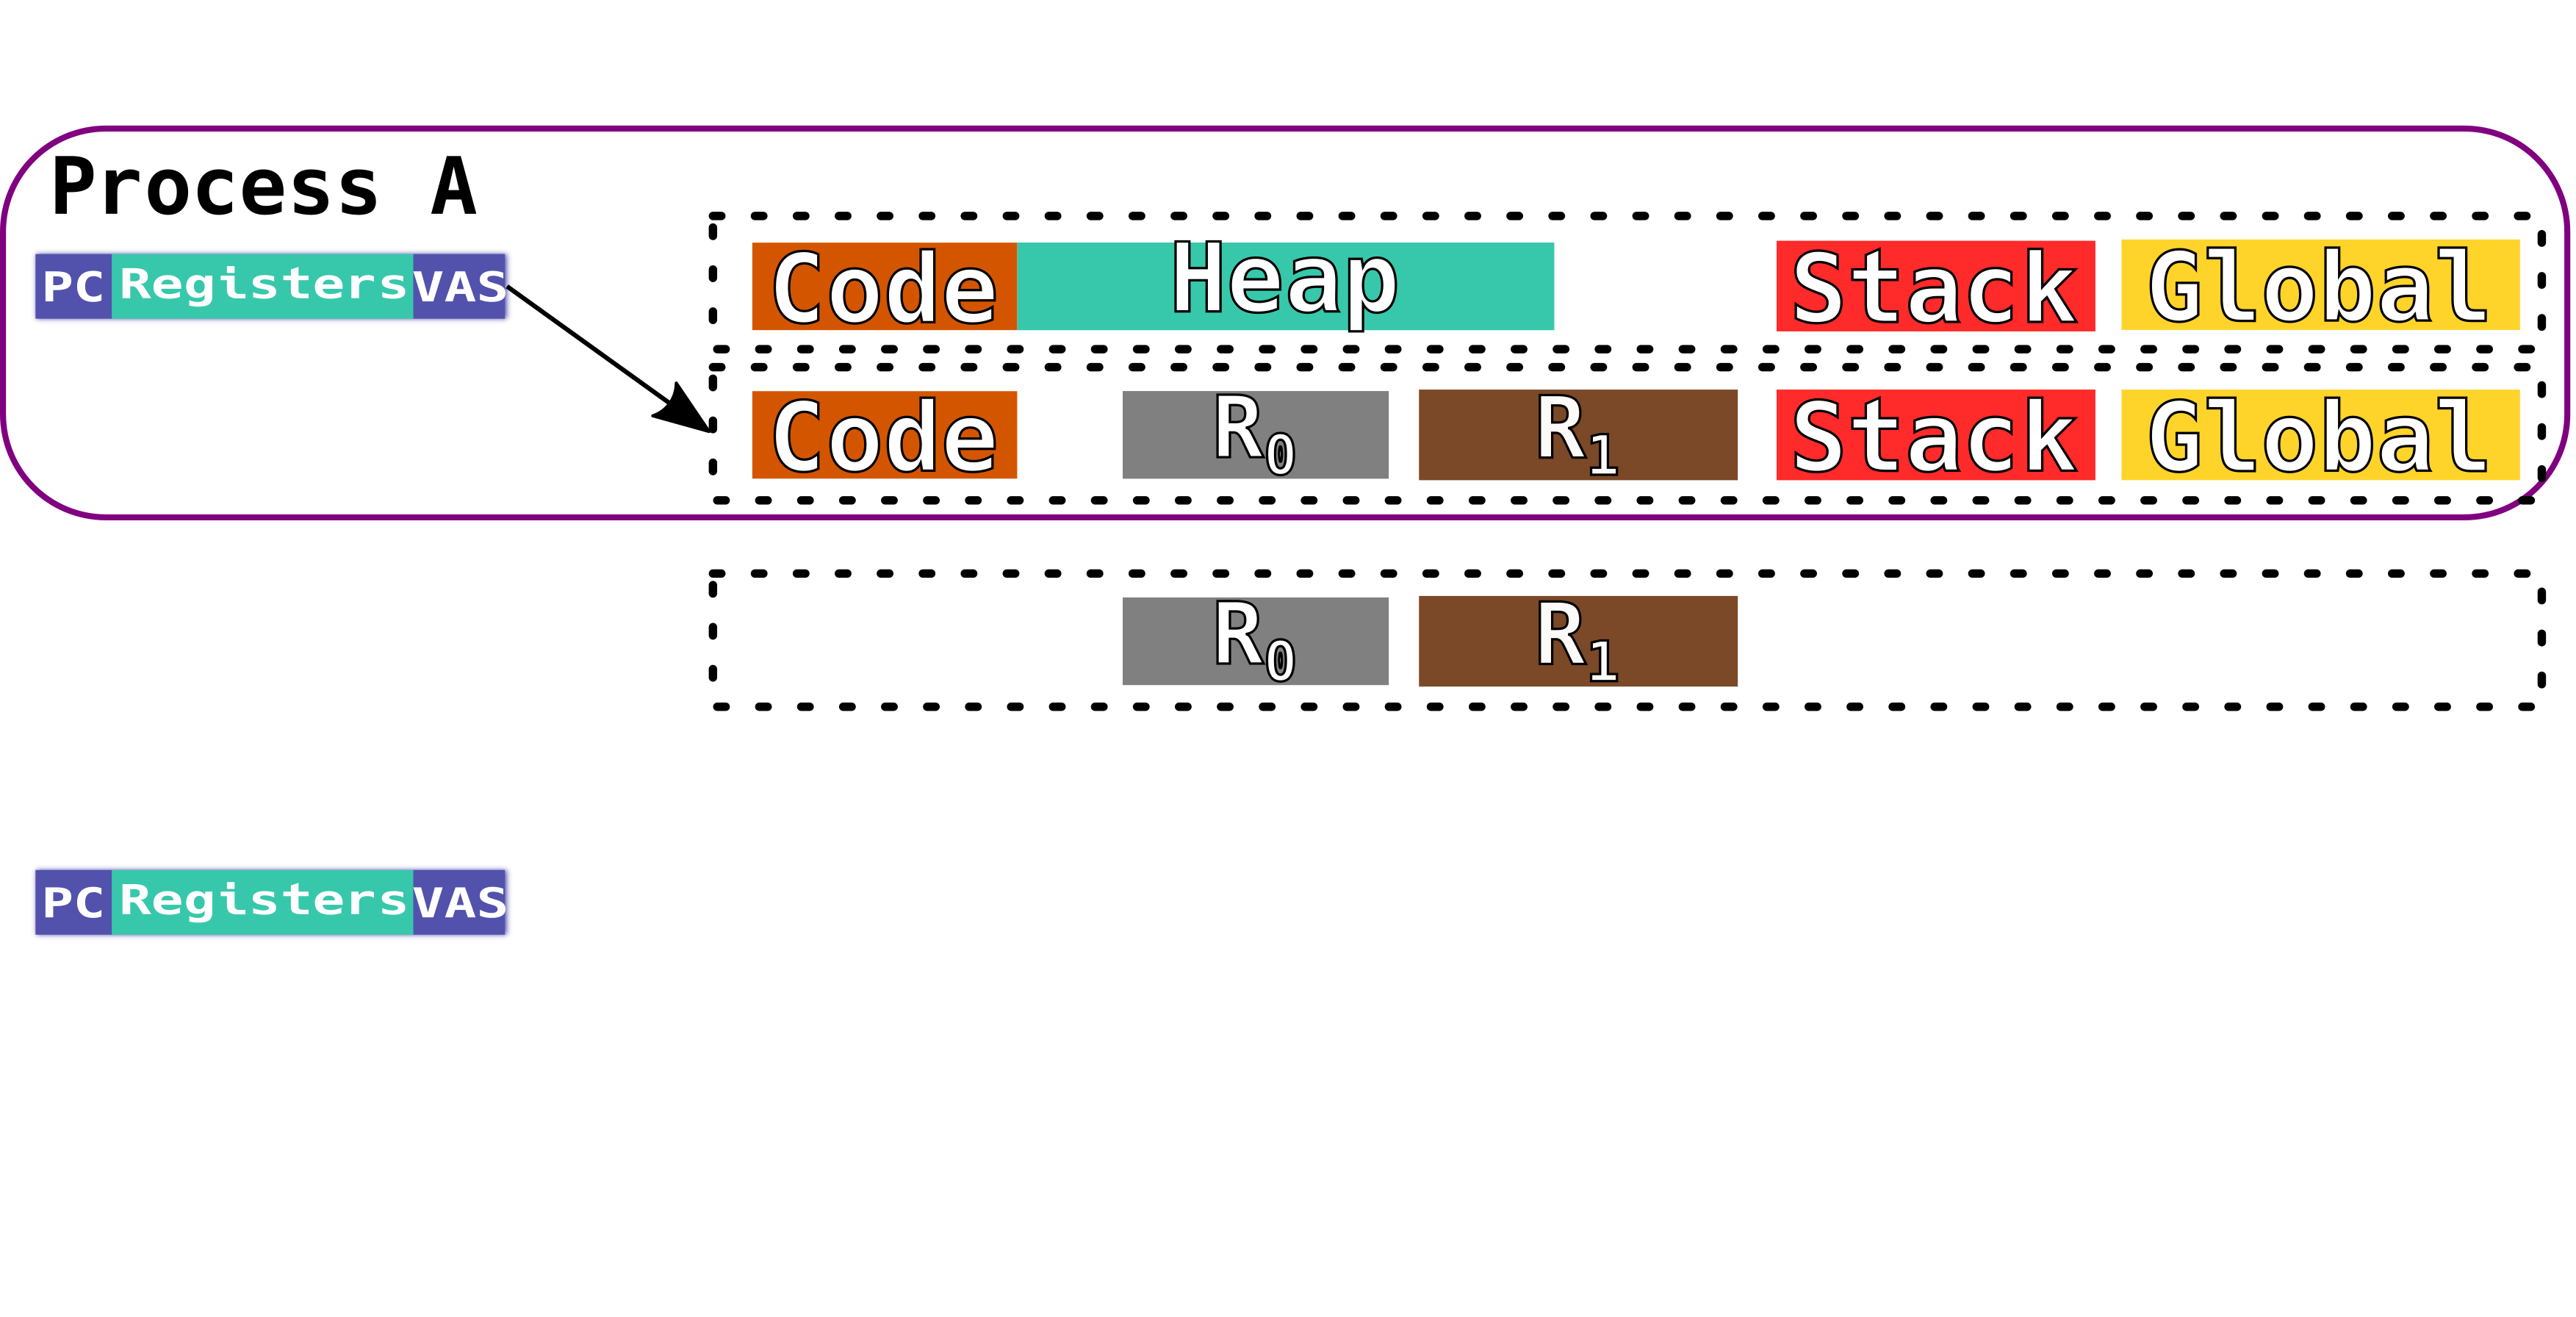
\includegraphics[width=1\textwidth, keepaspectratio=true]{images/spacejmp_example_g.png}
  \end{figure}
\end{frame}

\begin{frame}{Example}{Example}
  \begin{figure}[ht]
    \centering
    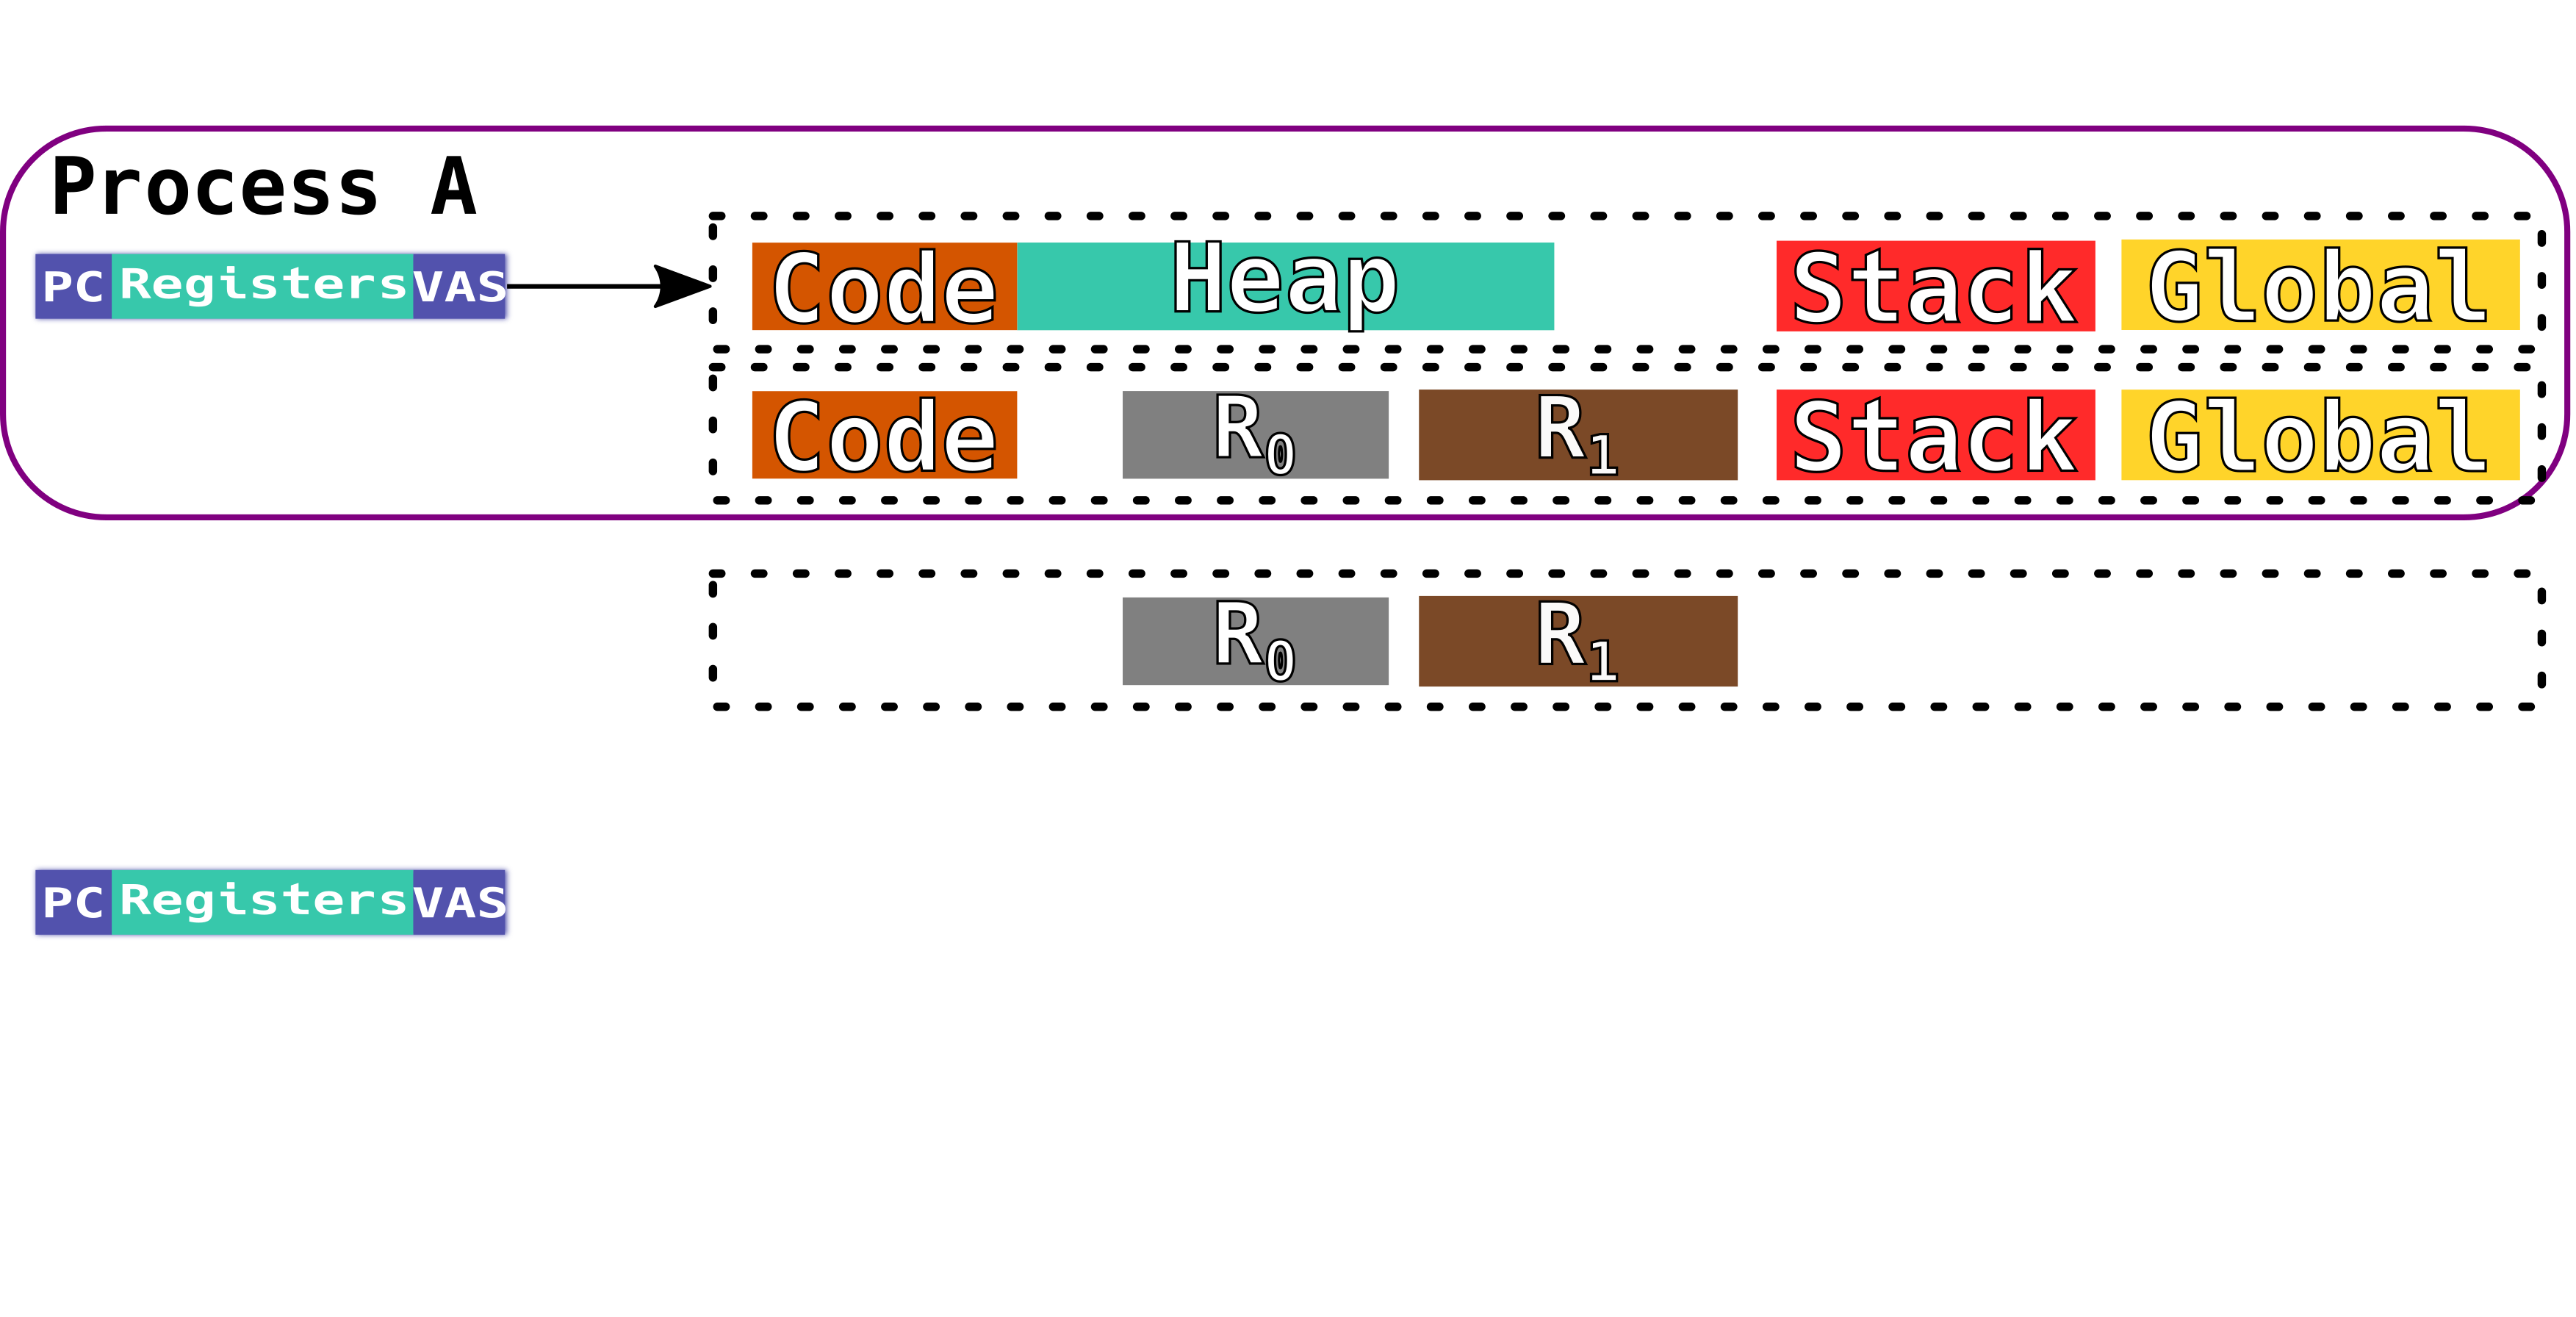
\includegraphics[width=1\textwidth, keepaspectratio=true]{images/spacejmp_example_f.png}
  \end{figure}
\end{frame}

\begin{frame}{Example}{Example}
  \begin{figure}[ht]
    \centering
    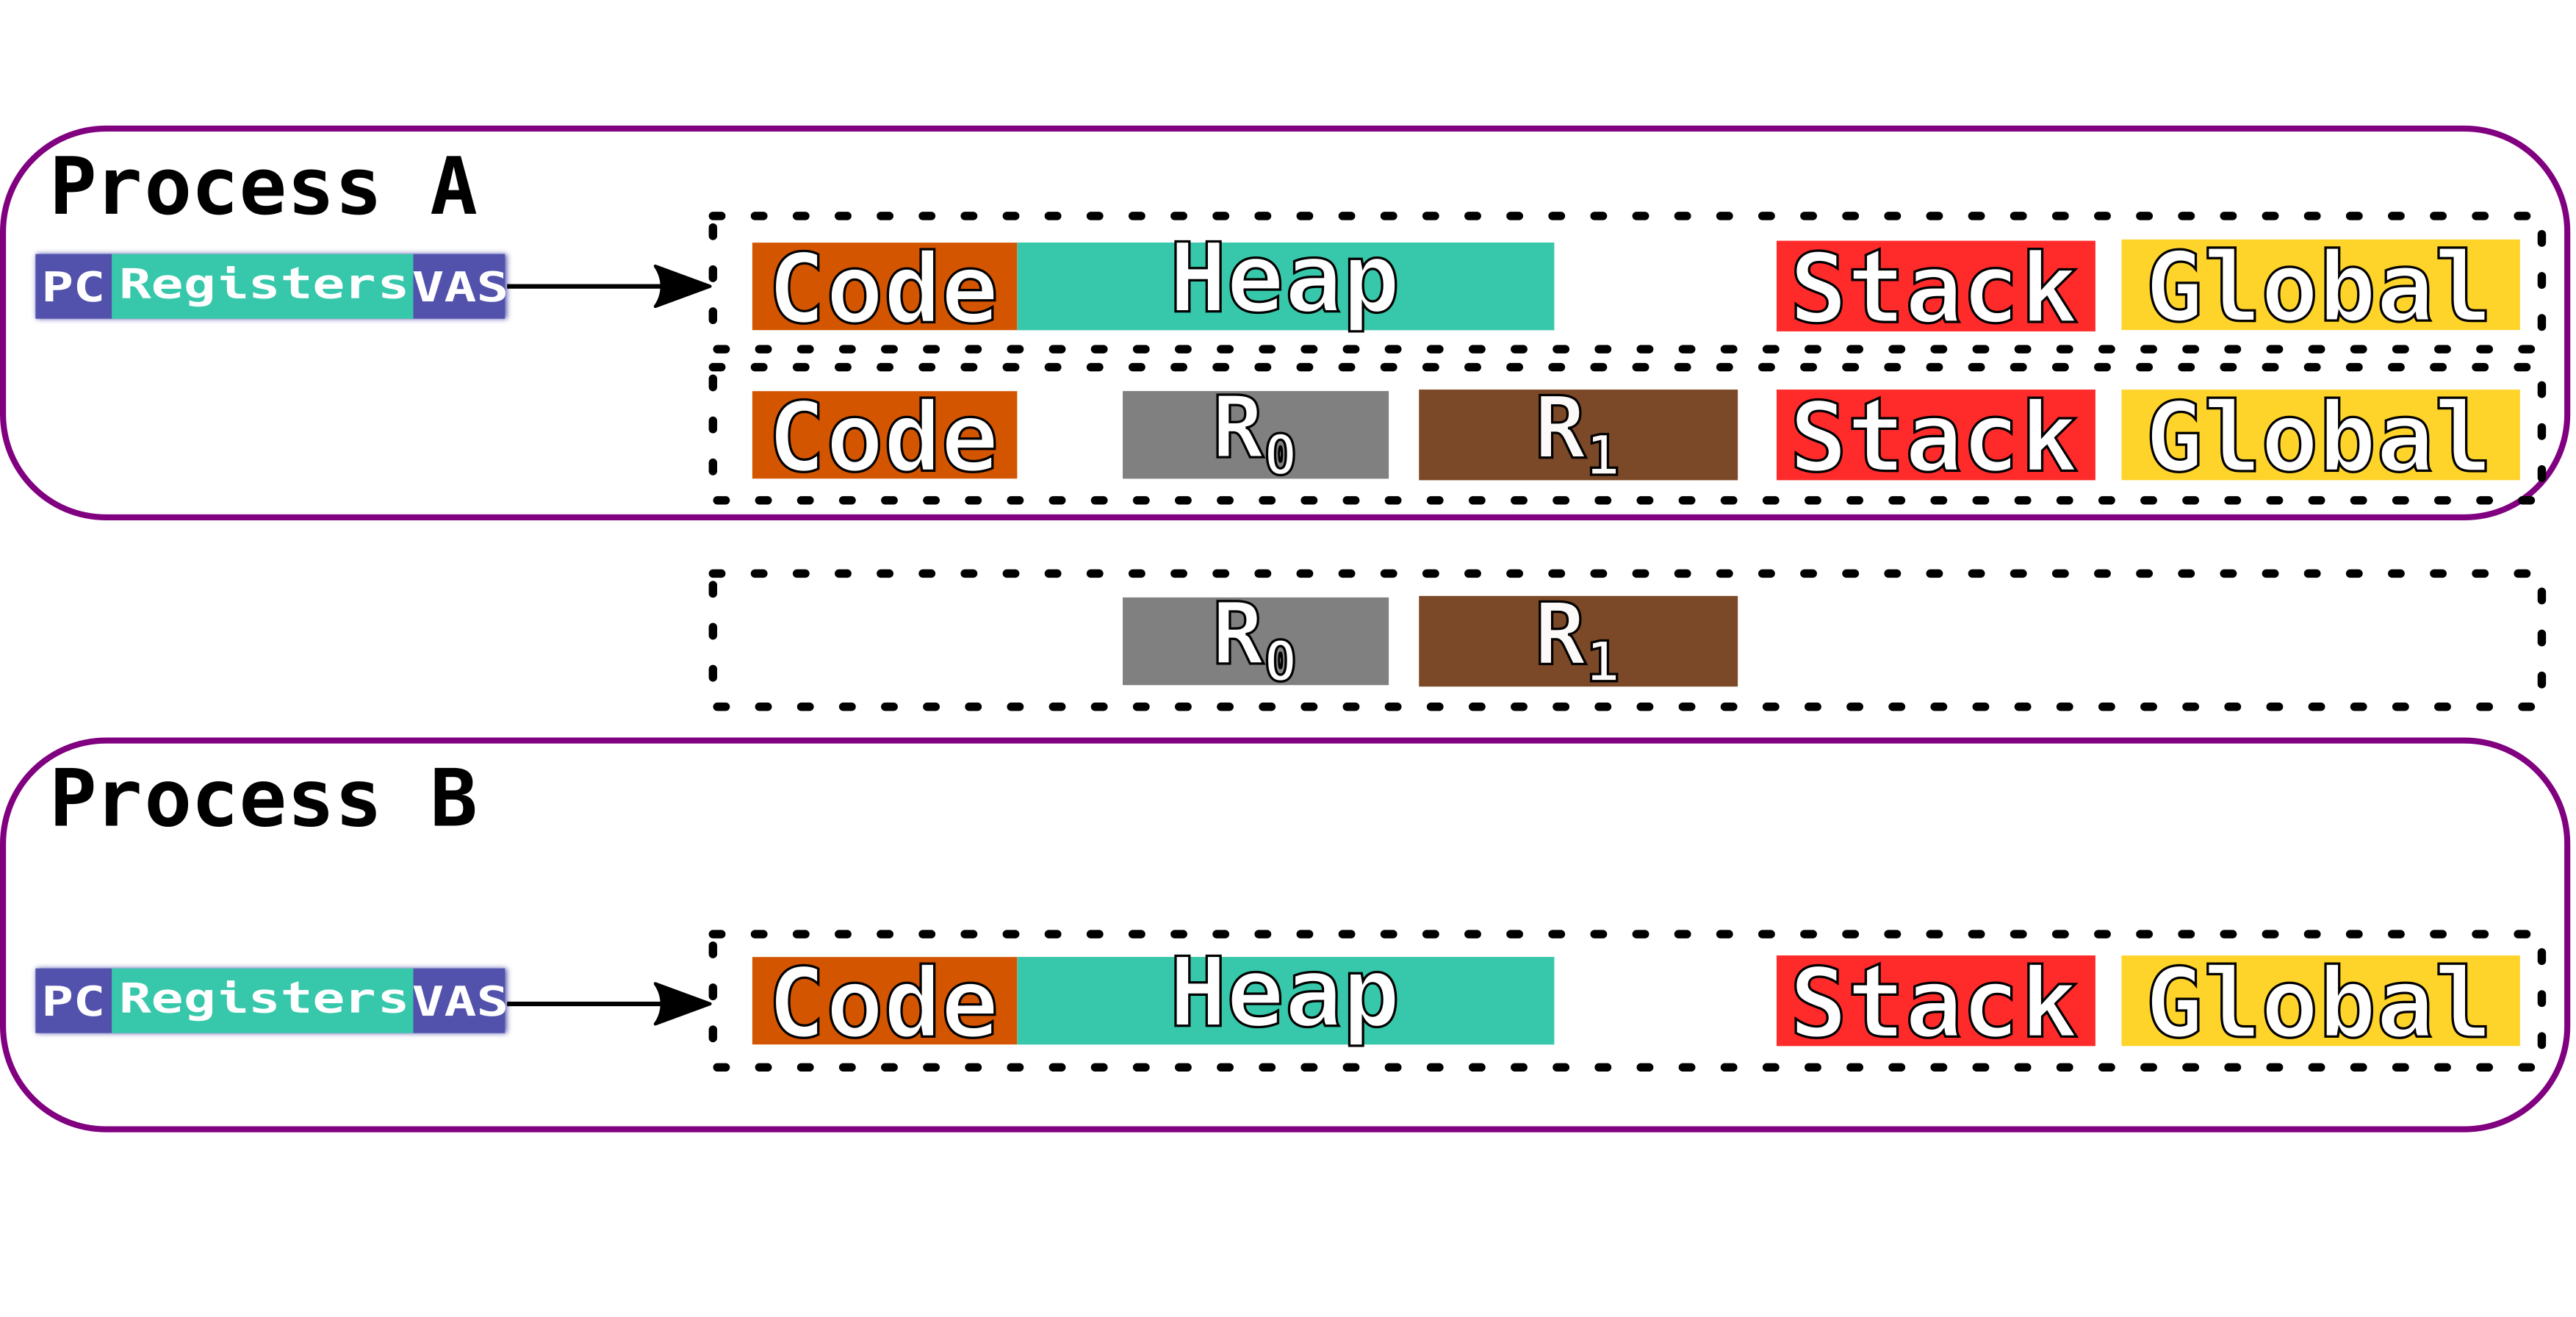
\includegraphics[width=1\textwidth, keepaspectratio=true]{images/spacejmp_example_h.png}
  \end{figure}
\end{frame}

\begin{frame}{Example}{Example}
  \begin{figure}[ht]
    \centering
    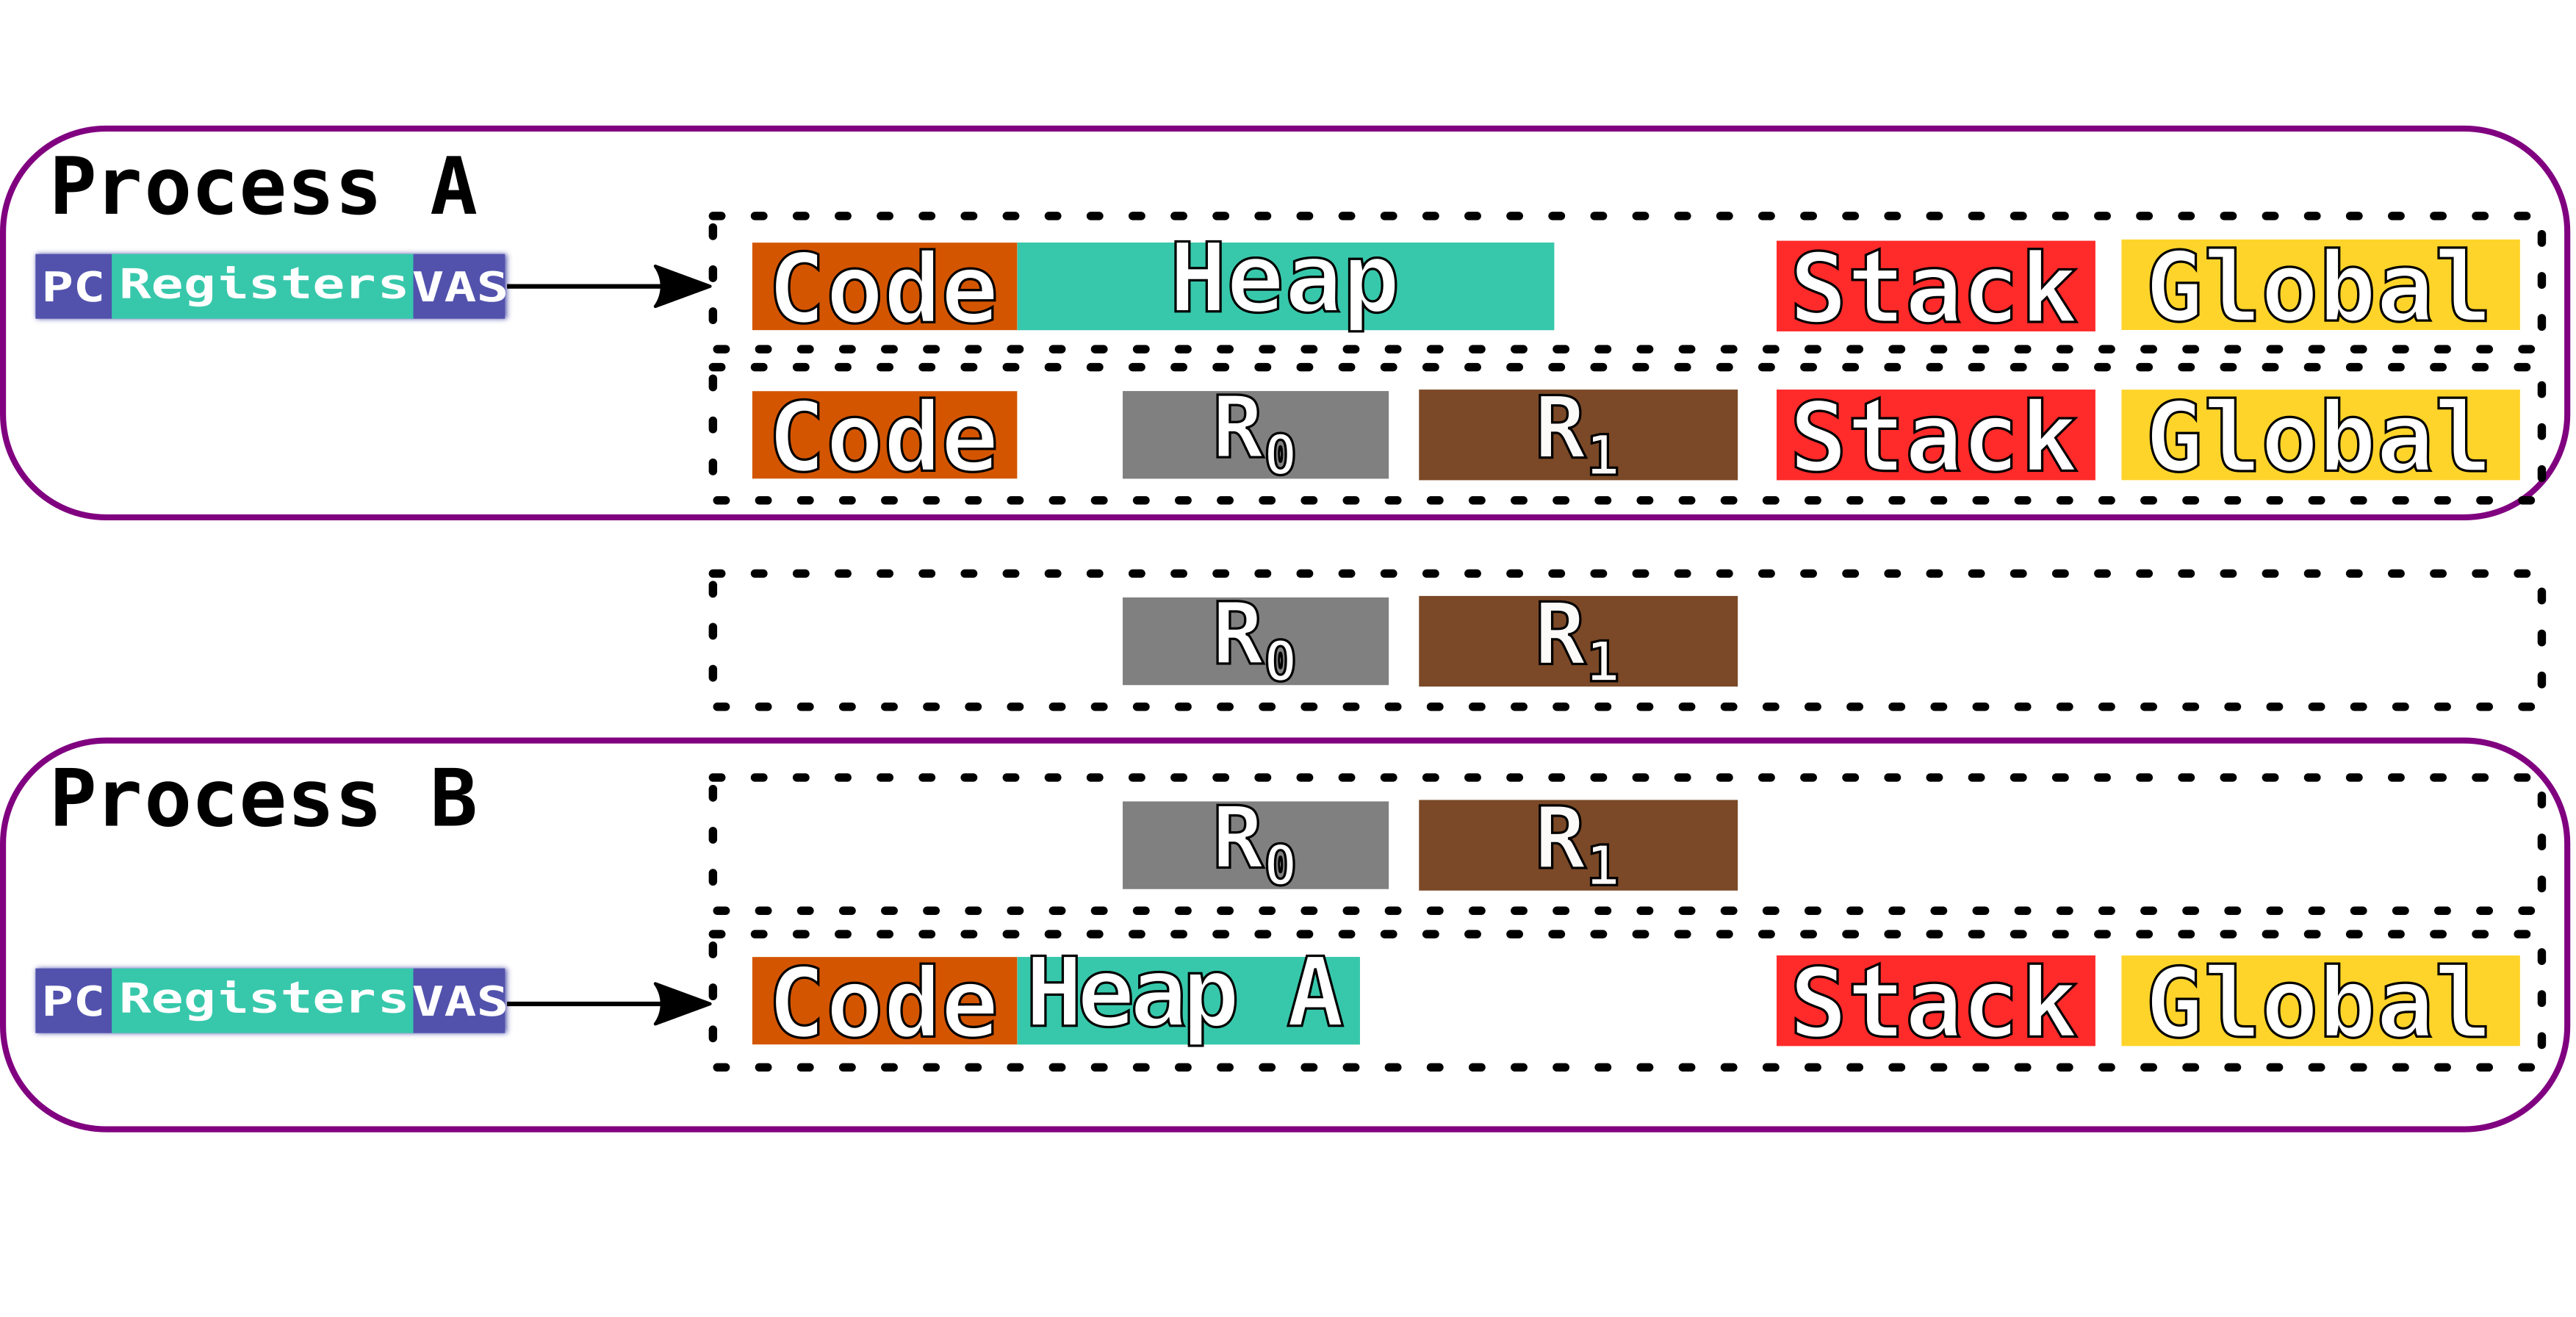
\includegraphics[width=1\textwidth, keepaspectratio=true]{images/spacejmp_example_i.png}
  \end{figure}
\end{frame}

\begin{frame}{Example}{Example}
  \begin{figure}[ht]
    \centering
    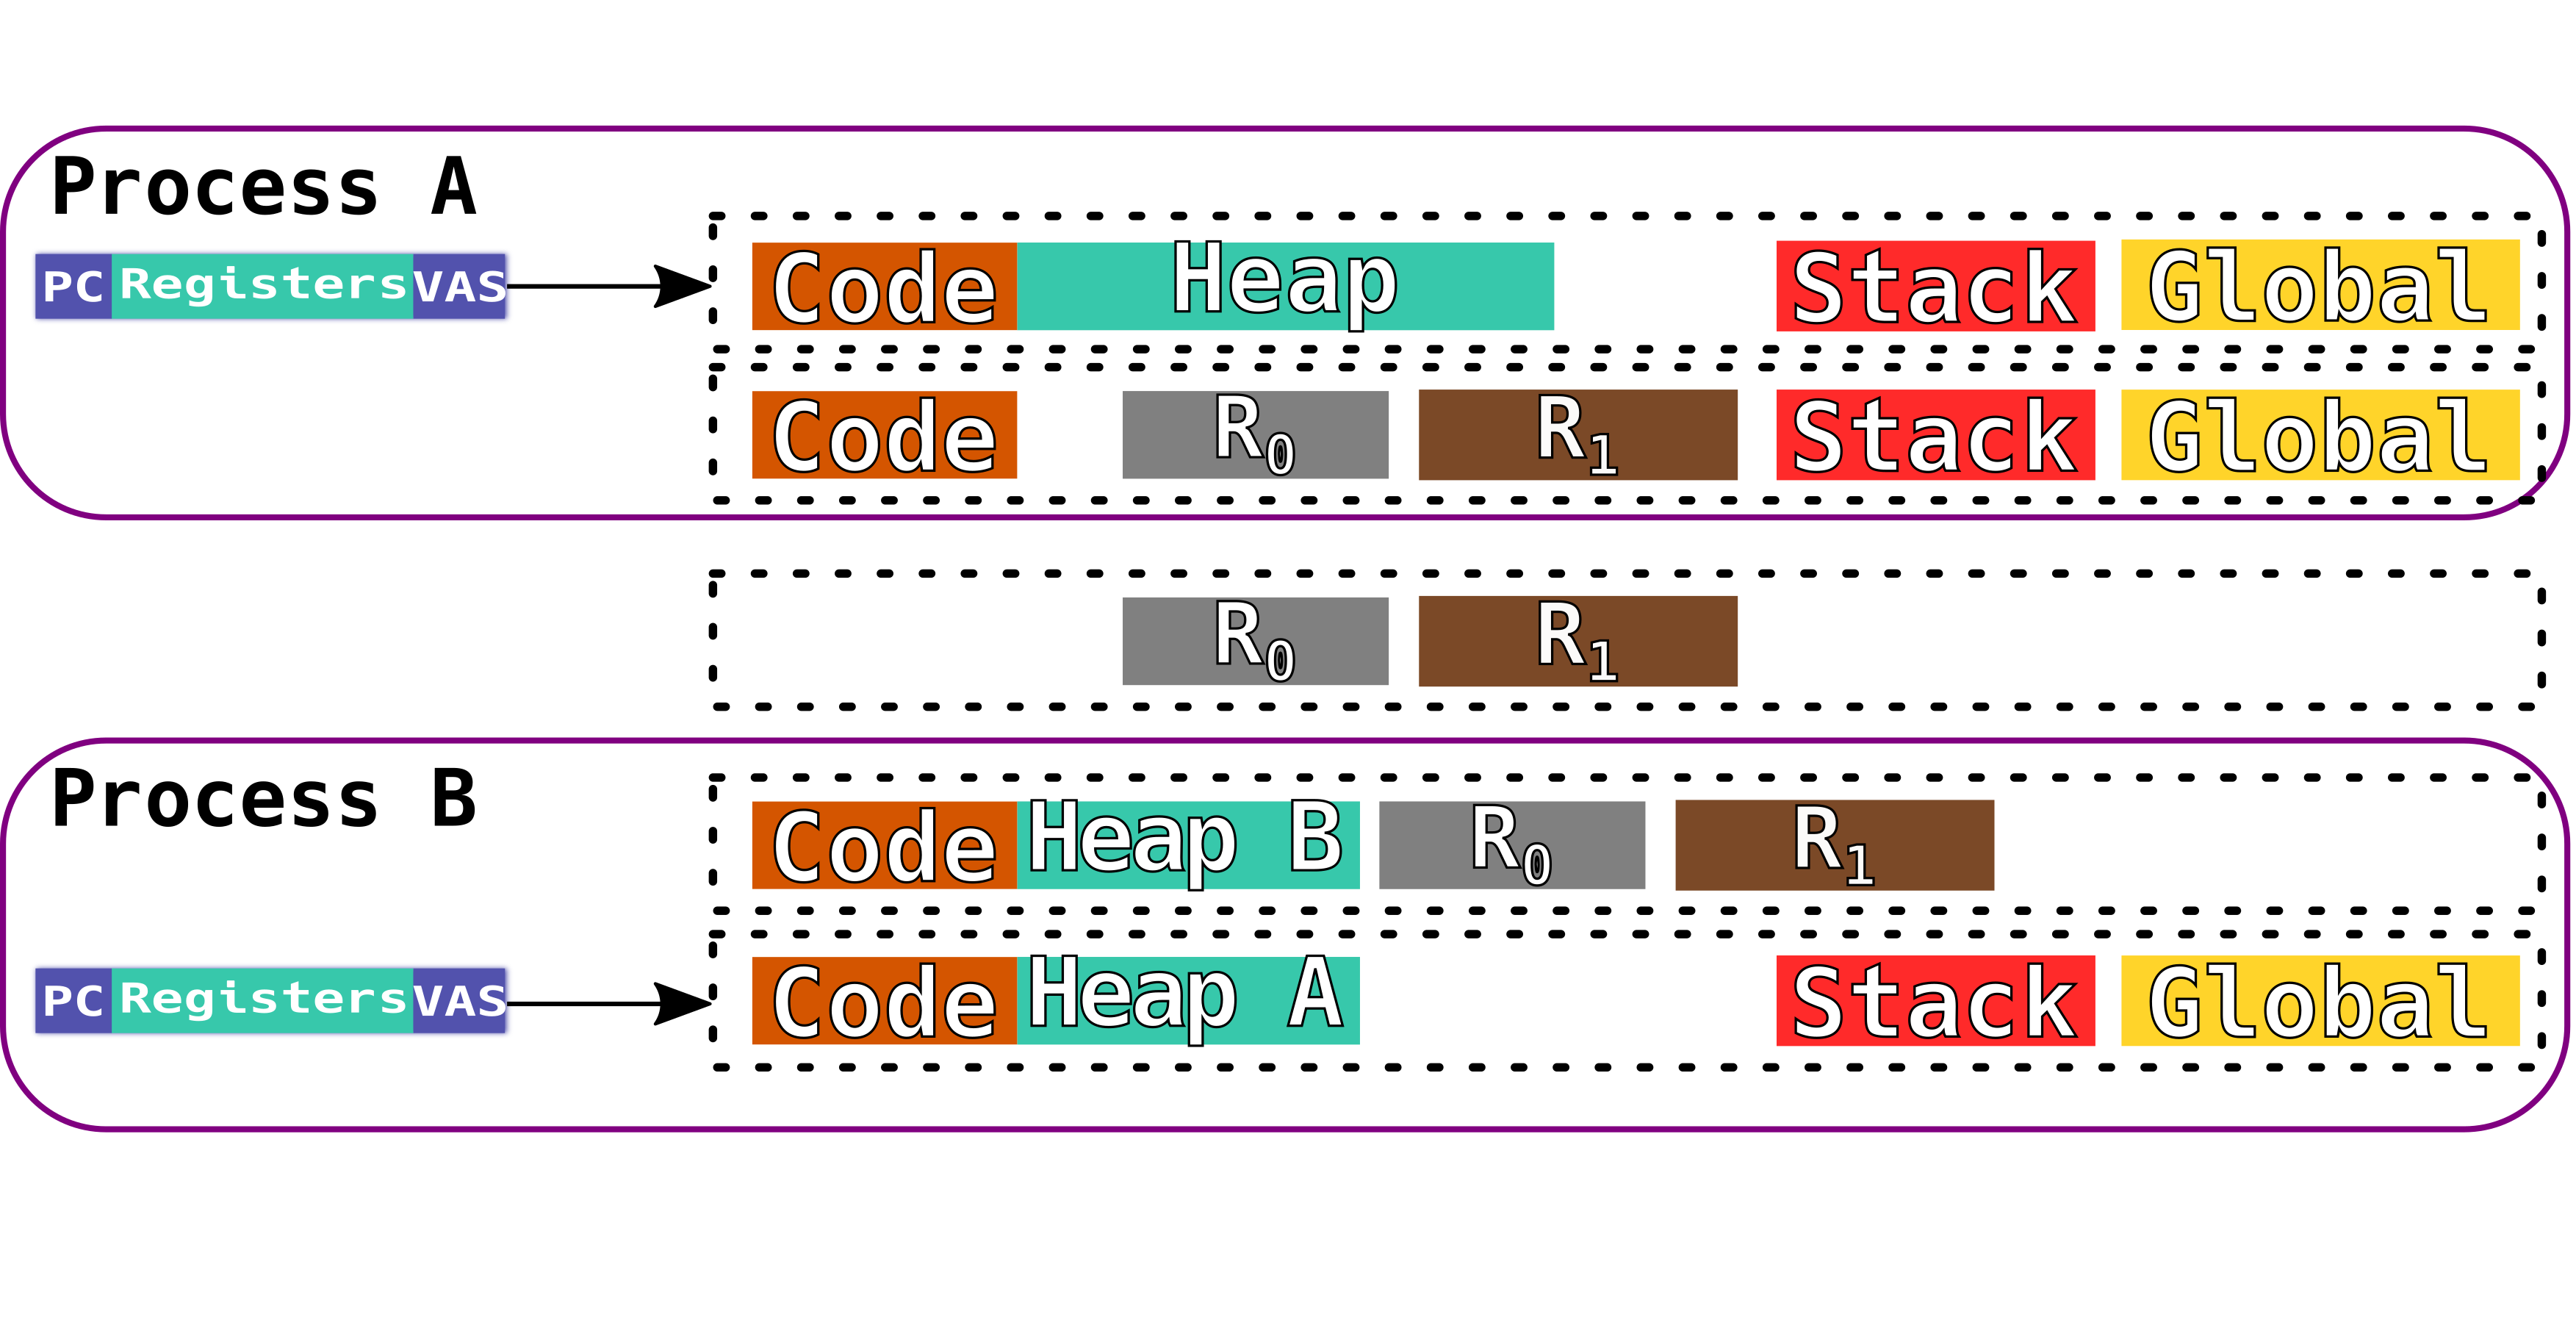
\includegraphics[width=1\textwidth, keepaspectratio=true]{images/spacejmp_example_j.png}
  \end{figure}
\end{frame}

\begin{frame}{Example}{Example}
  \begin{figure}[ht]
    \centering
    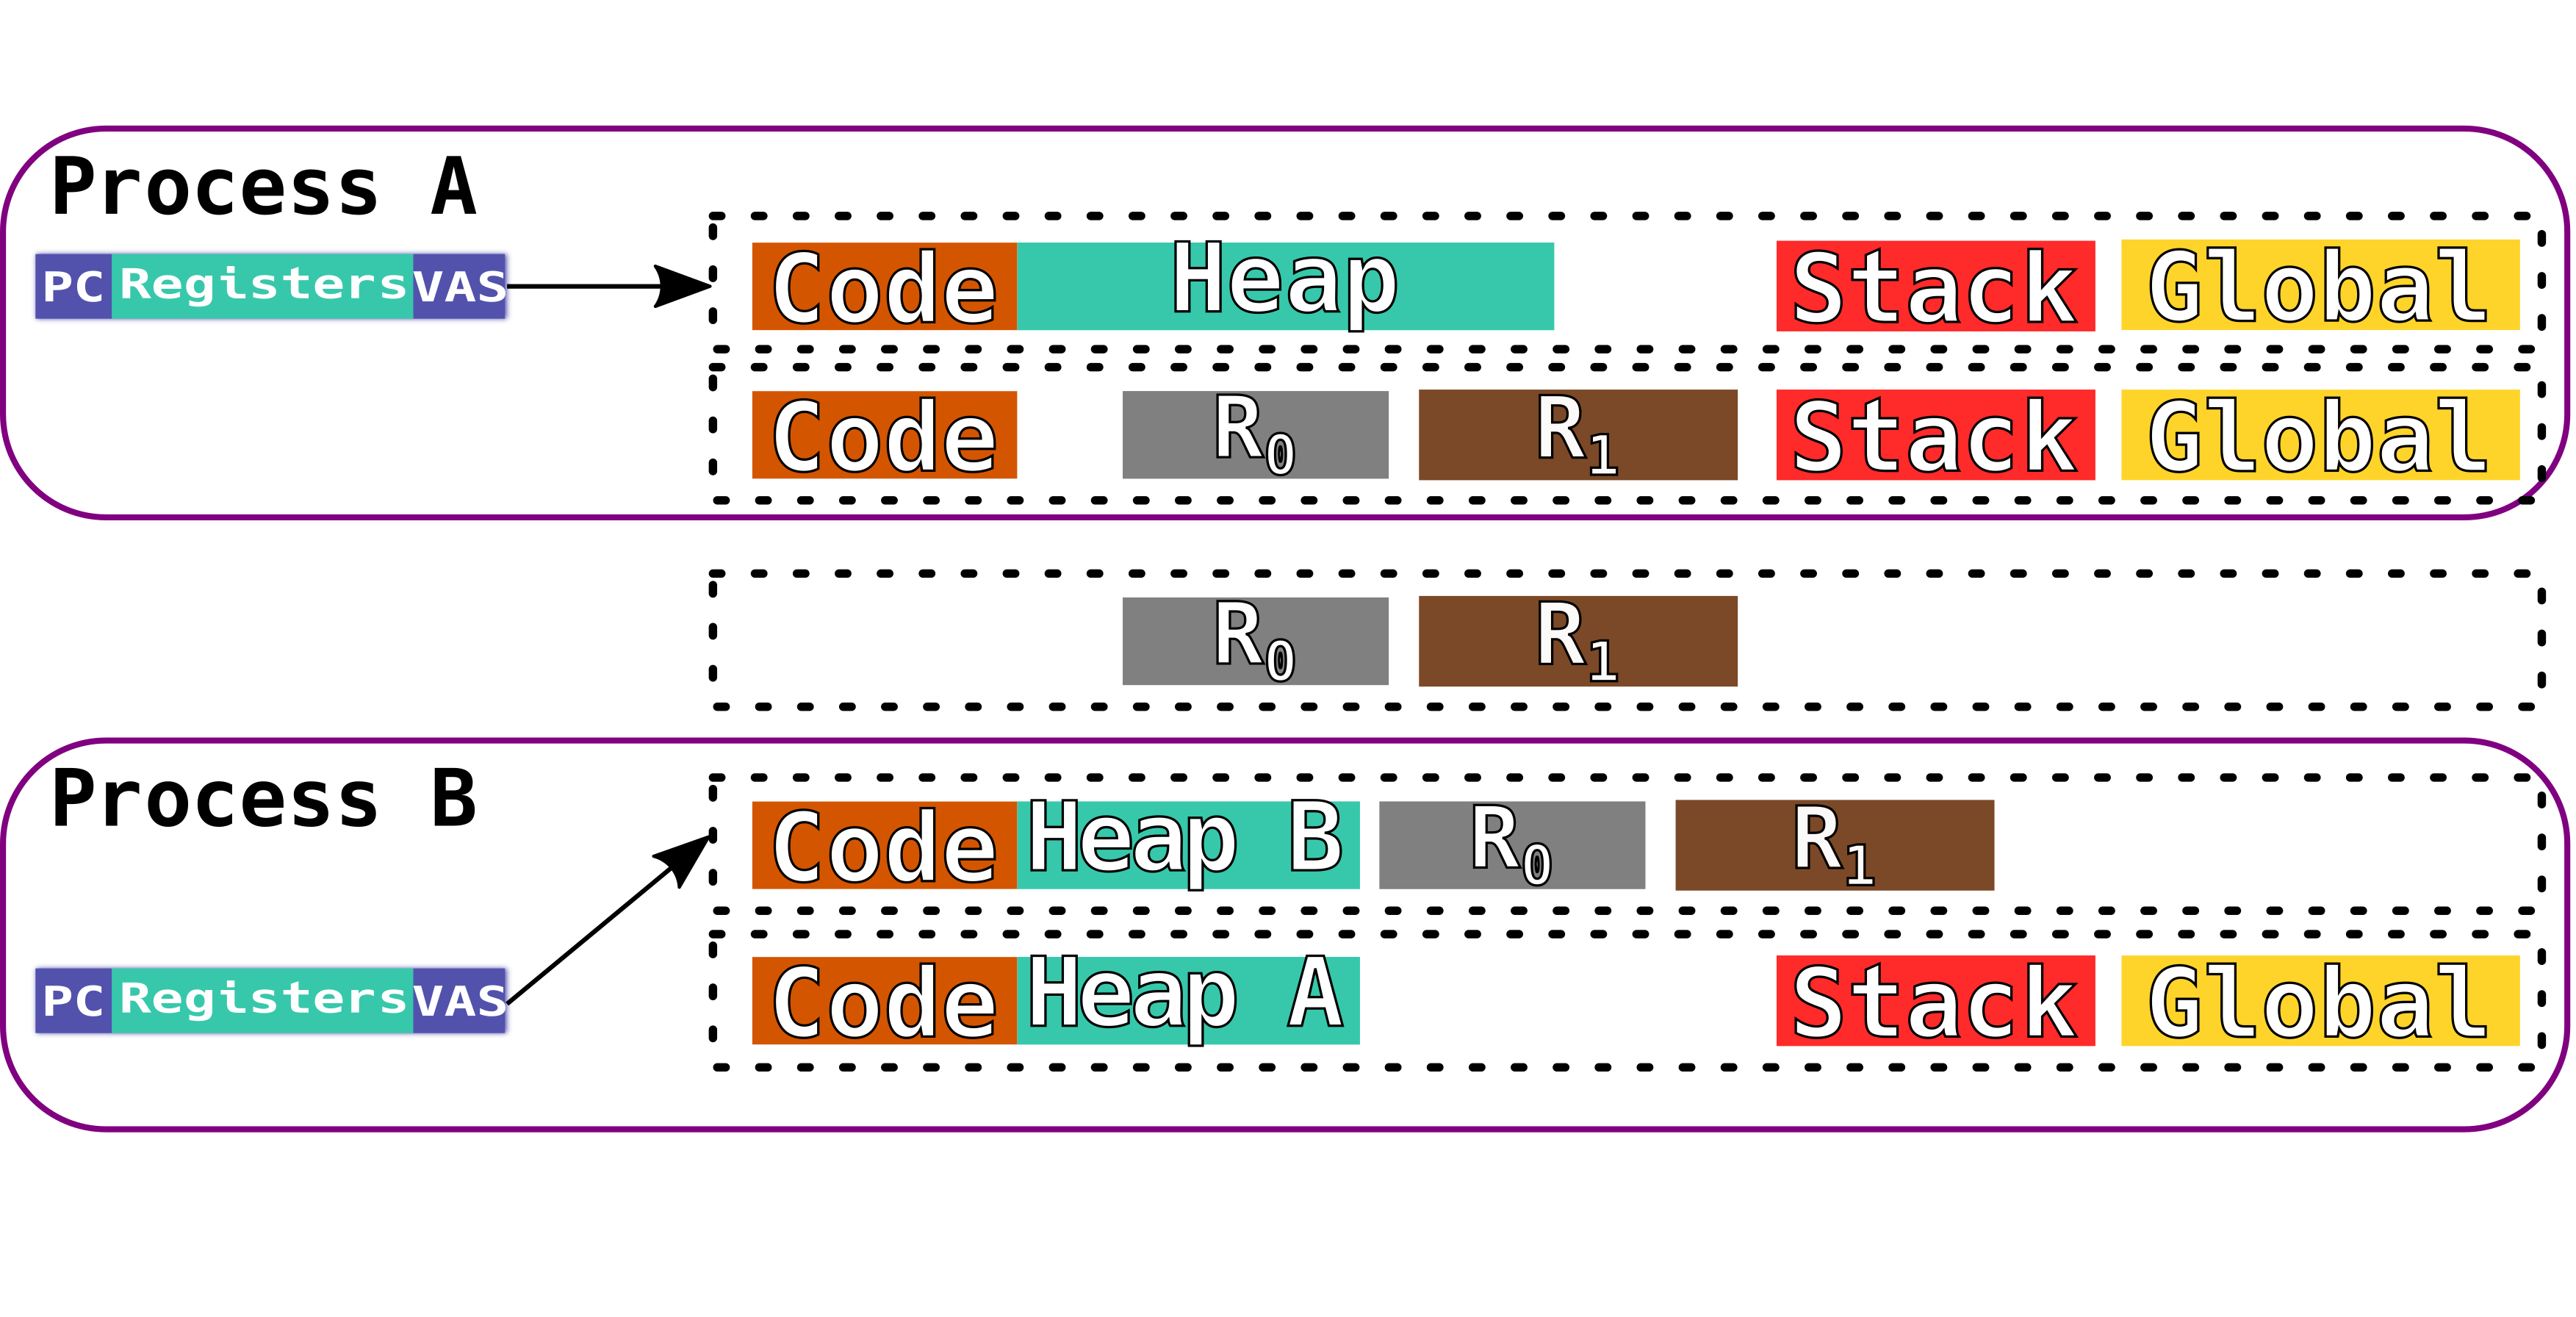
\includegraphics[width=1\textwidth, keepaspectratio=true]{images/spacejmp_example_k.png}
  \end{figure}
\end{frame}

\begin{frame}{Example}{Example}
  \begin{figure}[ht]
    \centering
    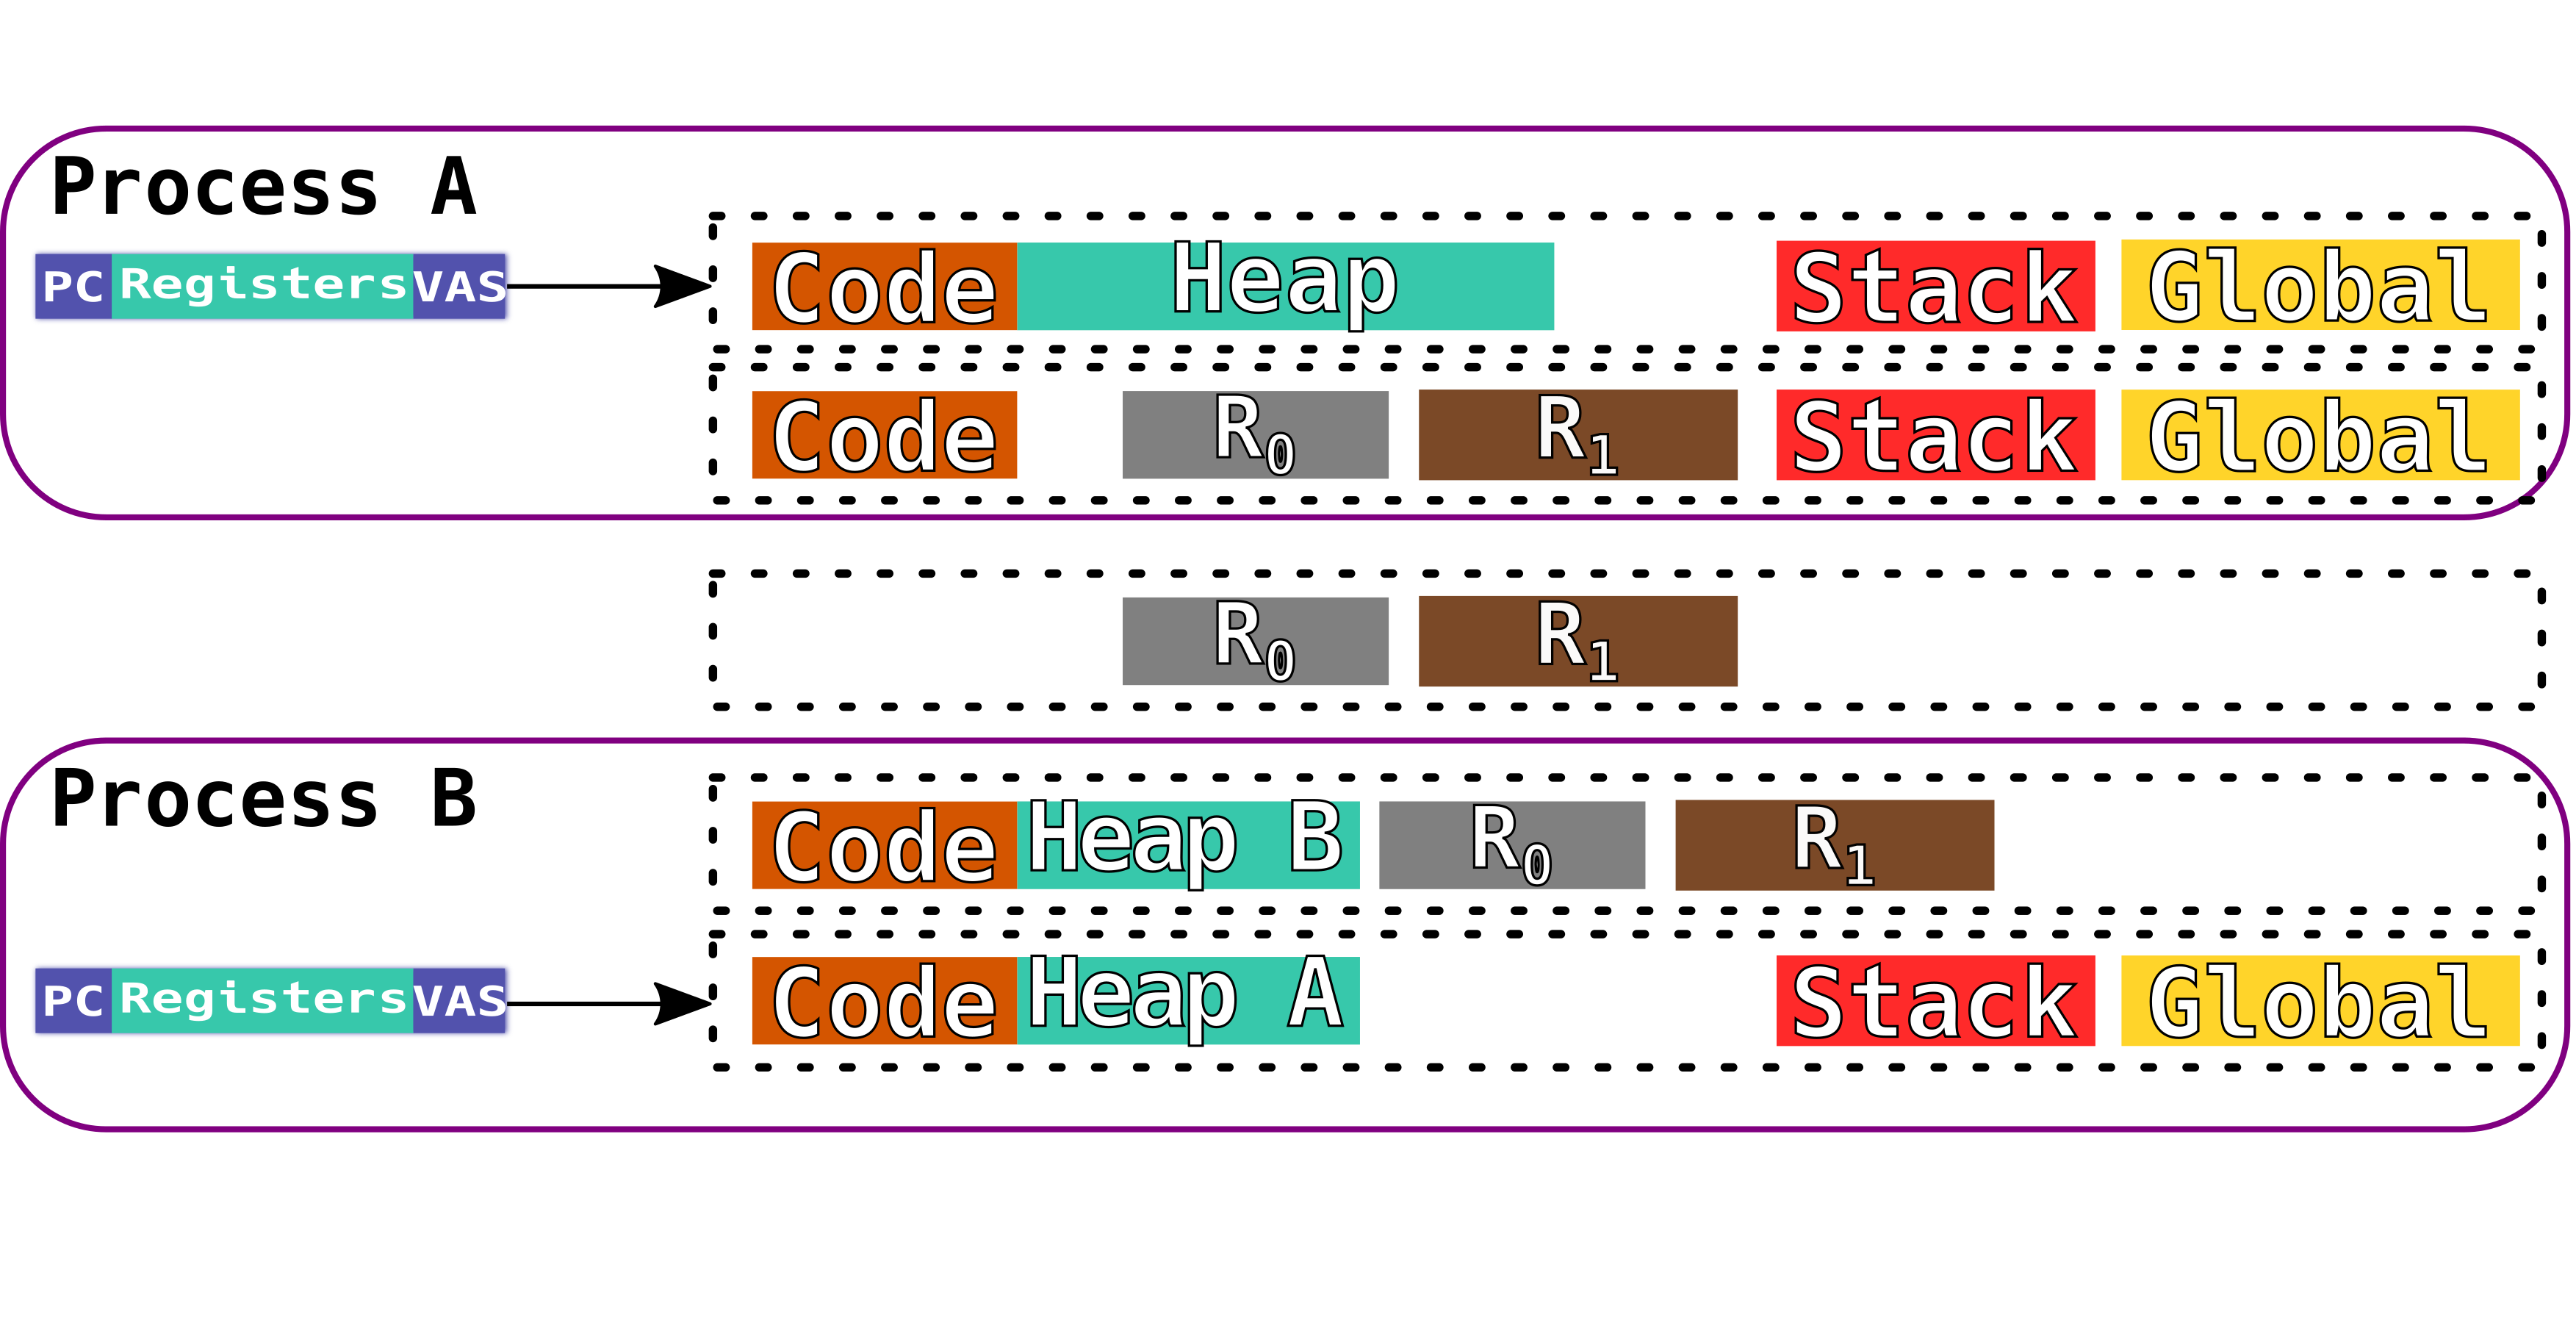
\includegraphics[width=1\textwidth, keepaspectratio=true]{images/spacejmp_example_l.png}
  \end{figure}
\end{frame}

\begin{frame}{Example}{Example}
  \begin{figure}[ht]
    \centering
    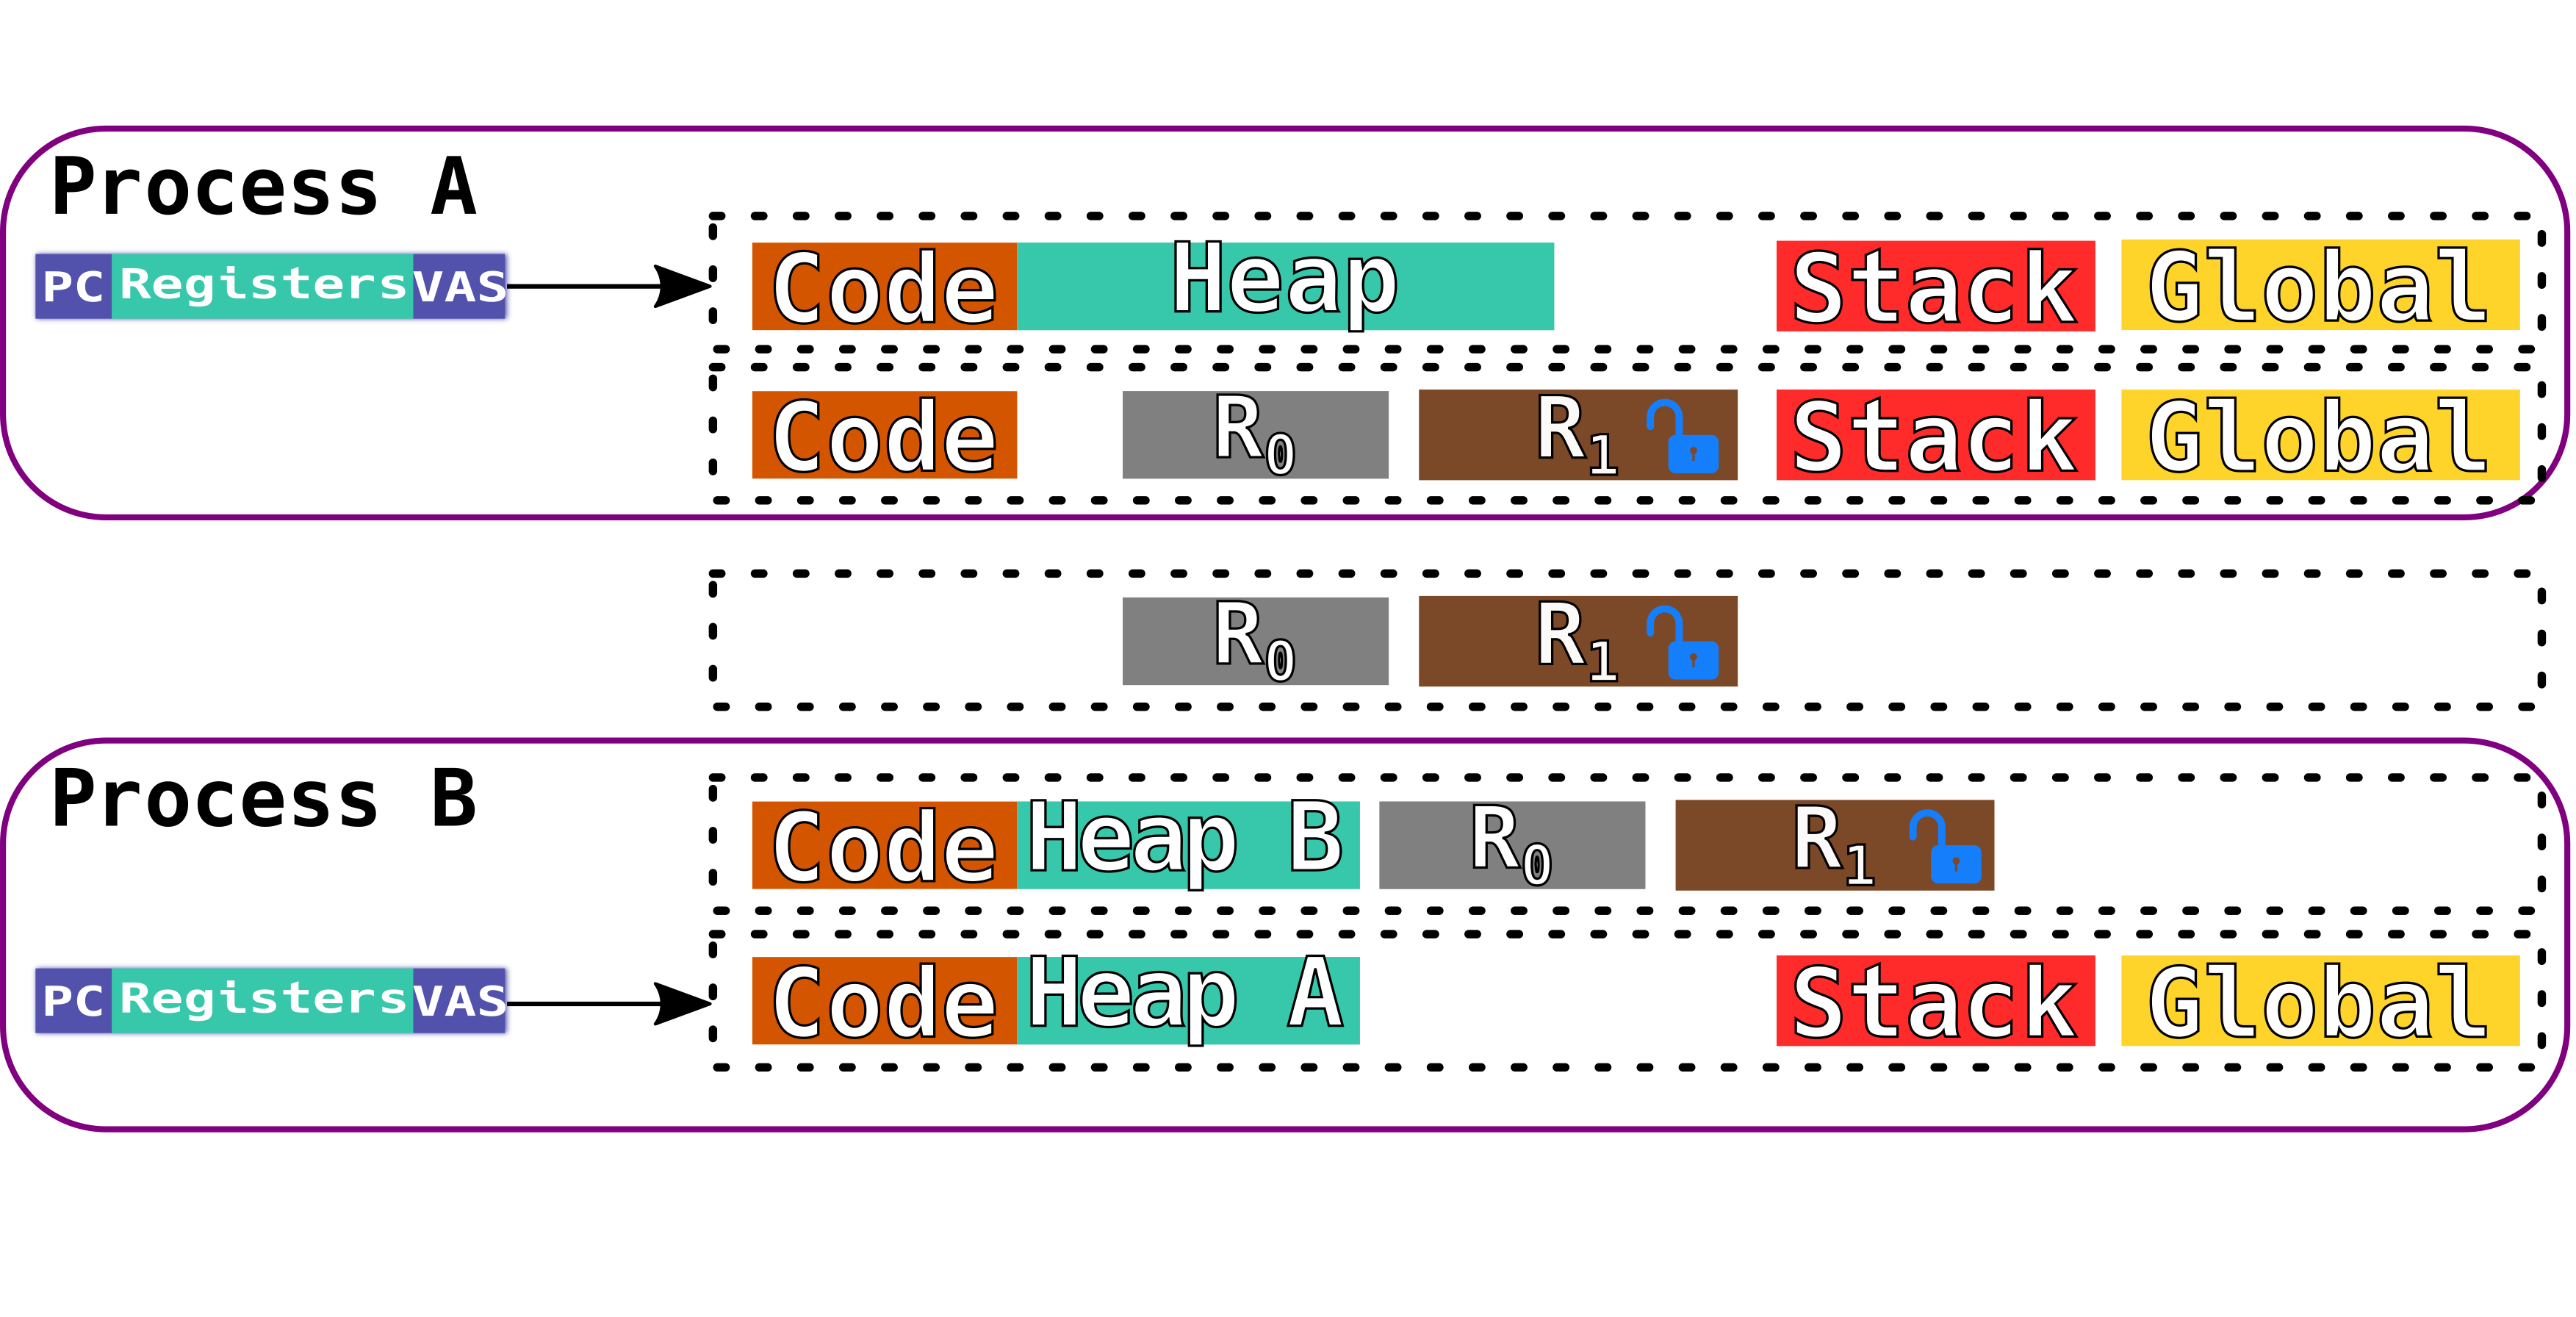
\includegraphics[width=1\textwidth, keepaspectratio=true]{images/spacejmp_example_m.png}
  \end{figure}
\end{frame}

\begin{frame}{Example}{Example}
  \begin{figure}[ht]
    \centering
    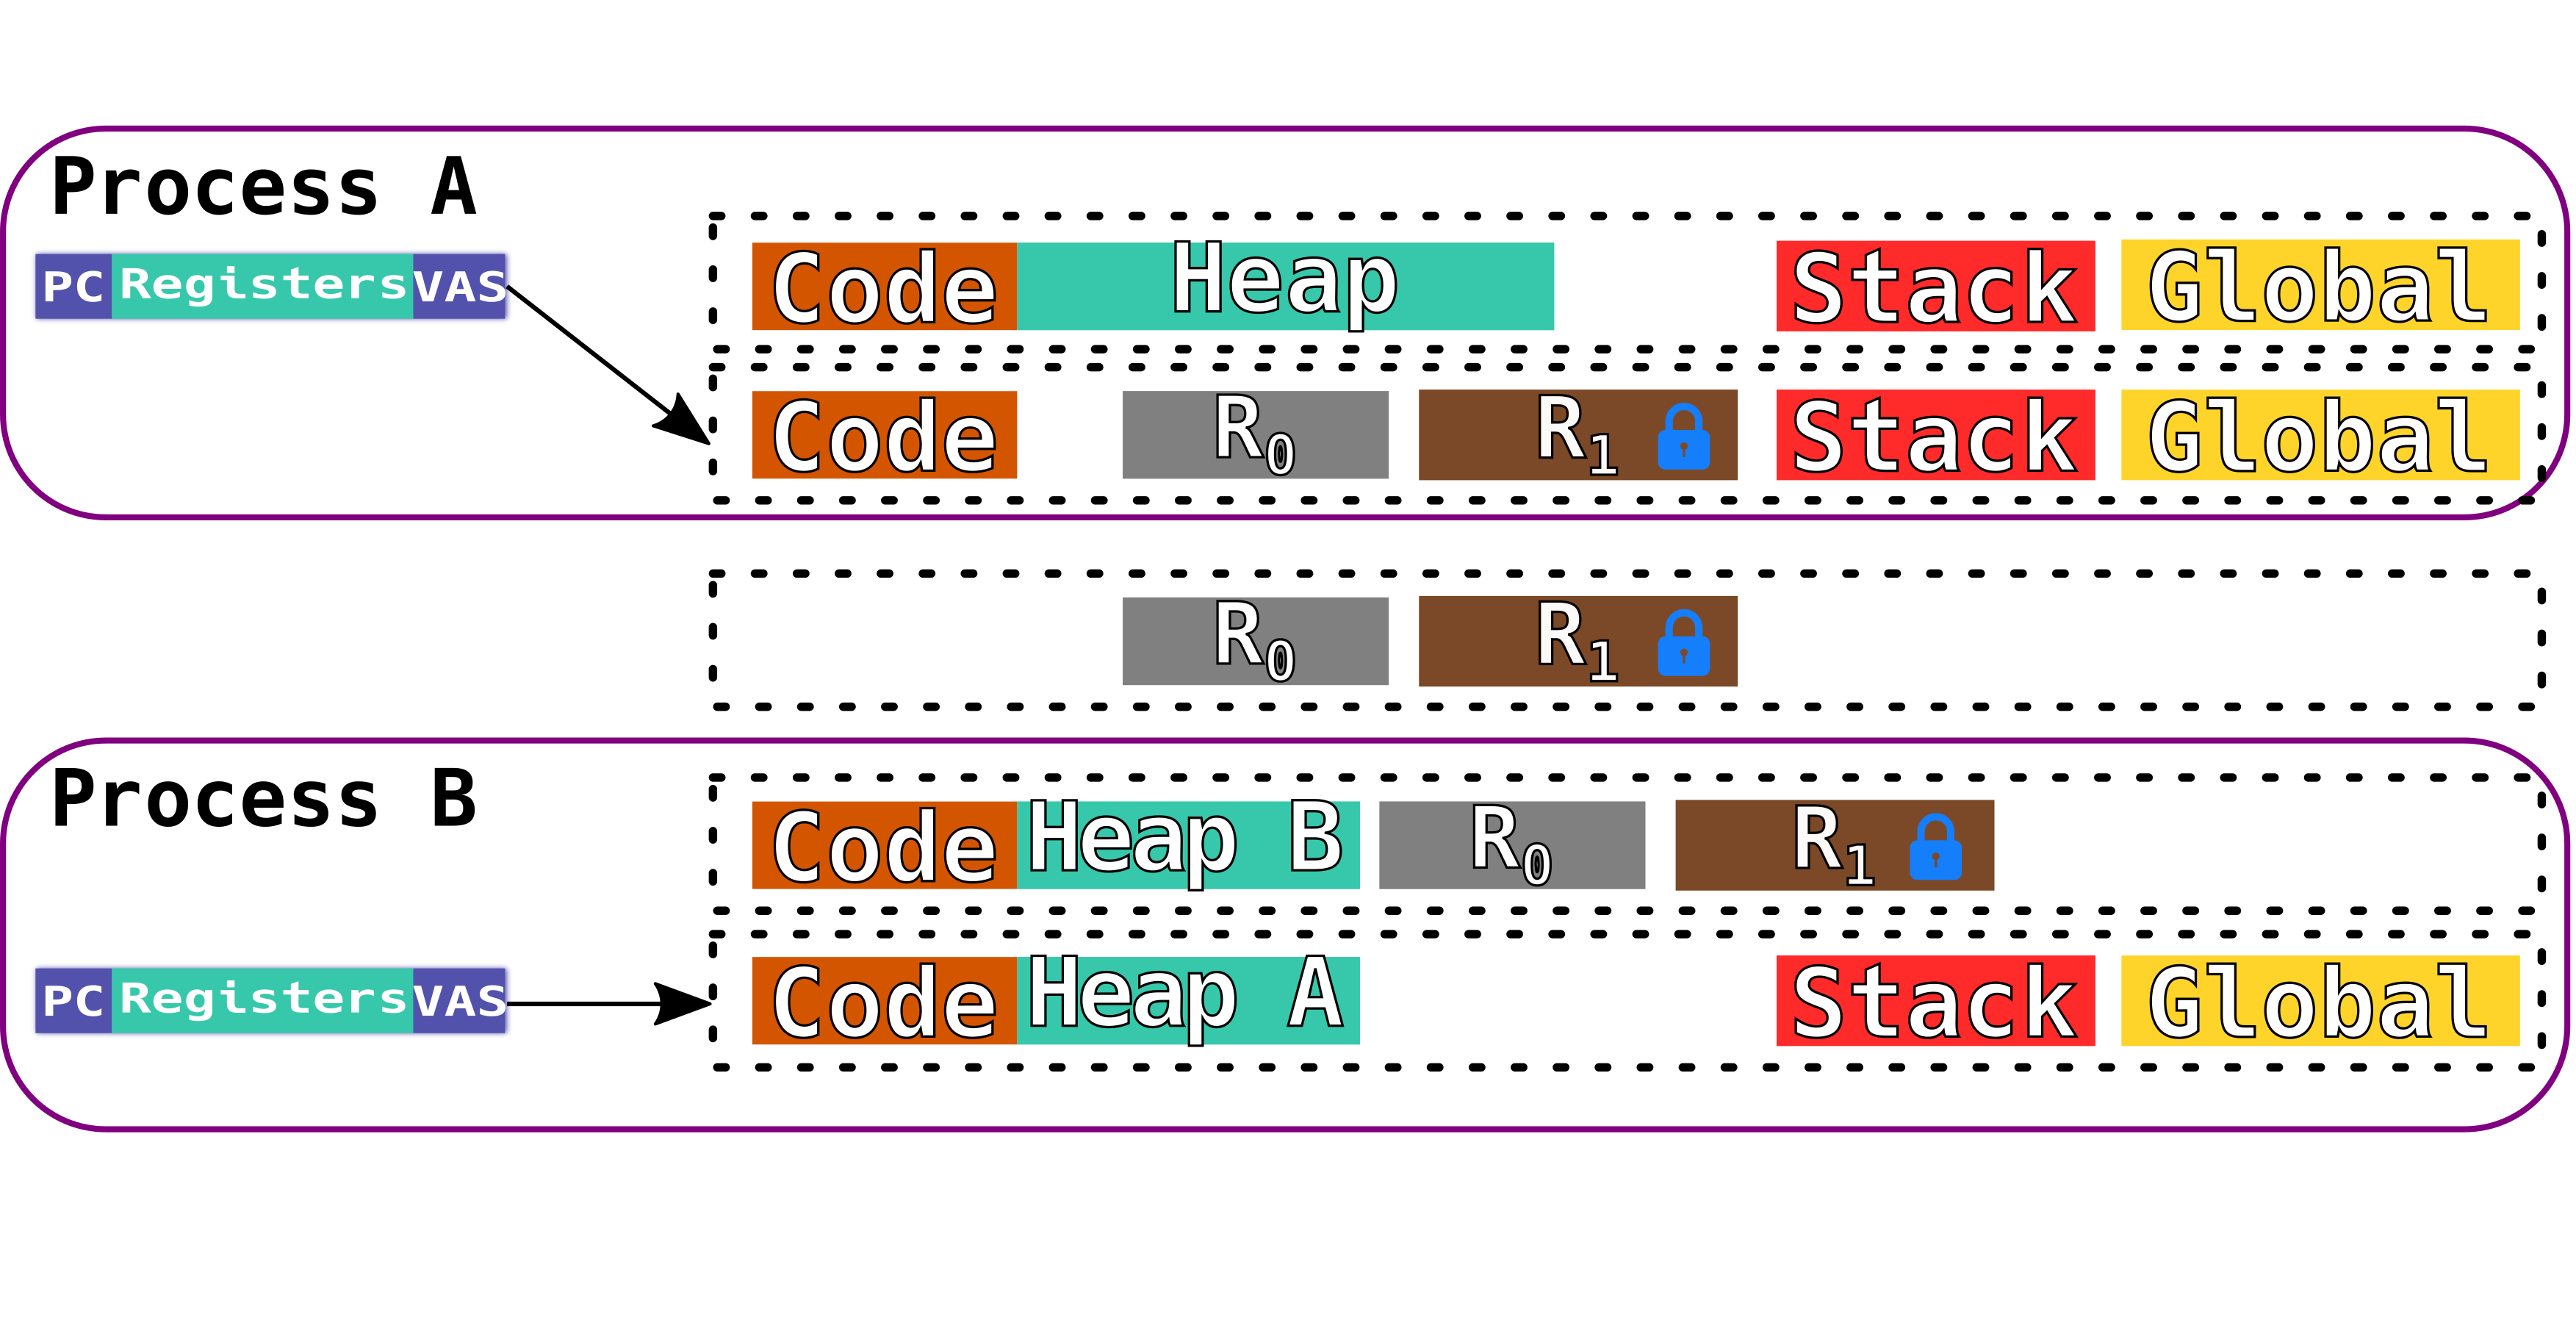
\includegraphics[width=1\textwidth, keepaspectratio=true]{images/spacejmp_example_n.png}
  \end{figure}
\end{frame}

\begin{frame}{Example}{Example}
  \begin{figure}[ht]
    \centering
    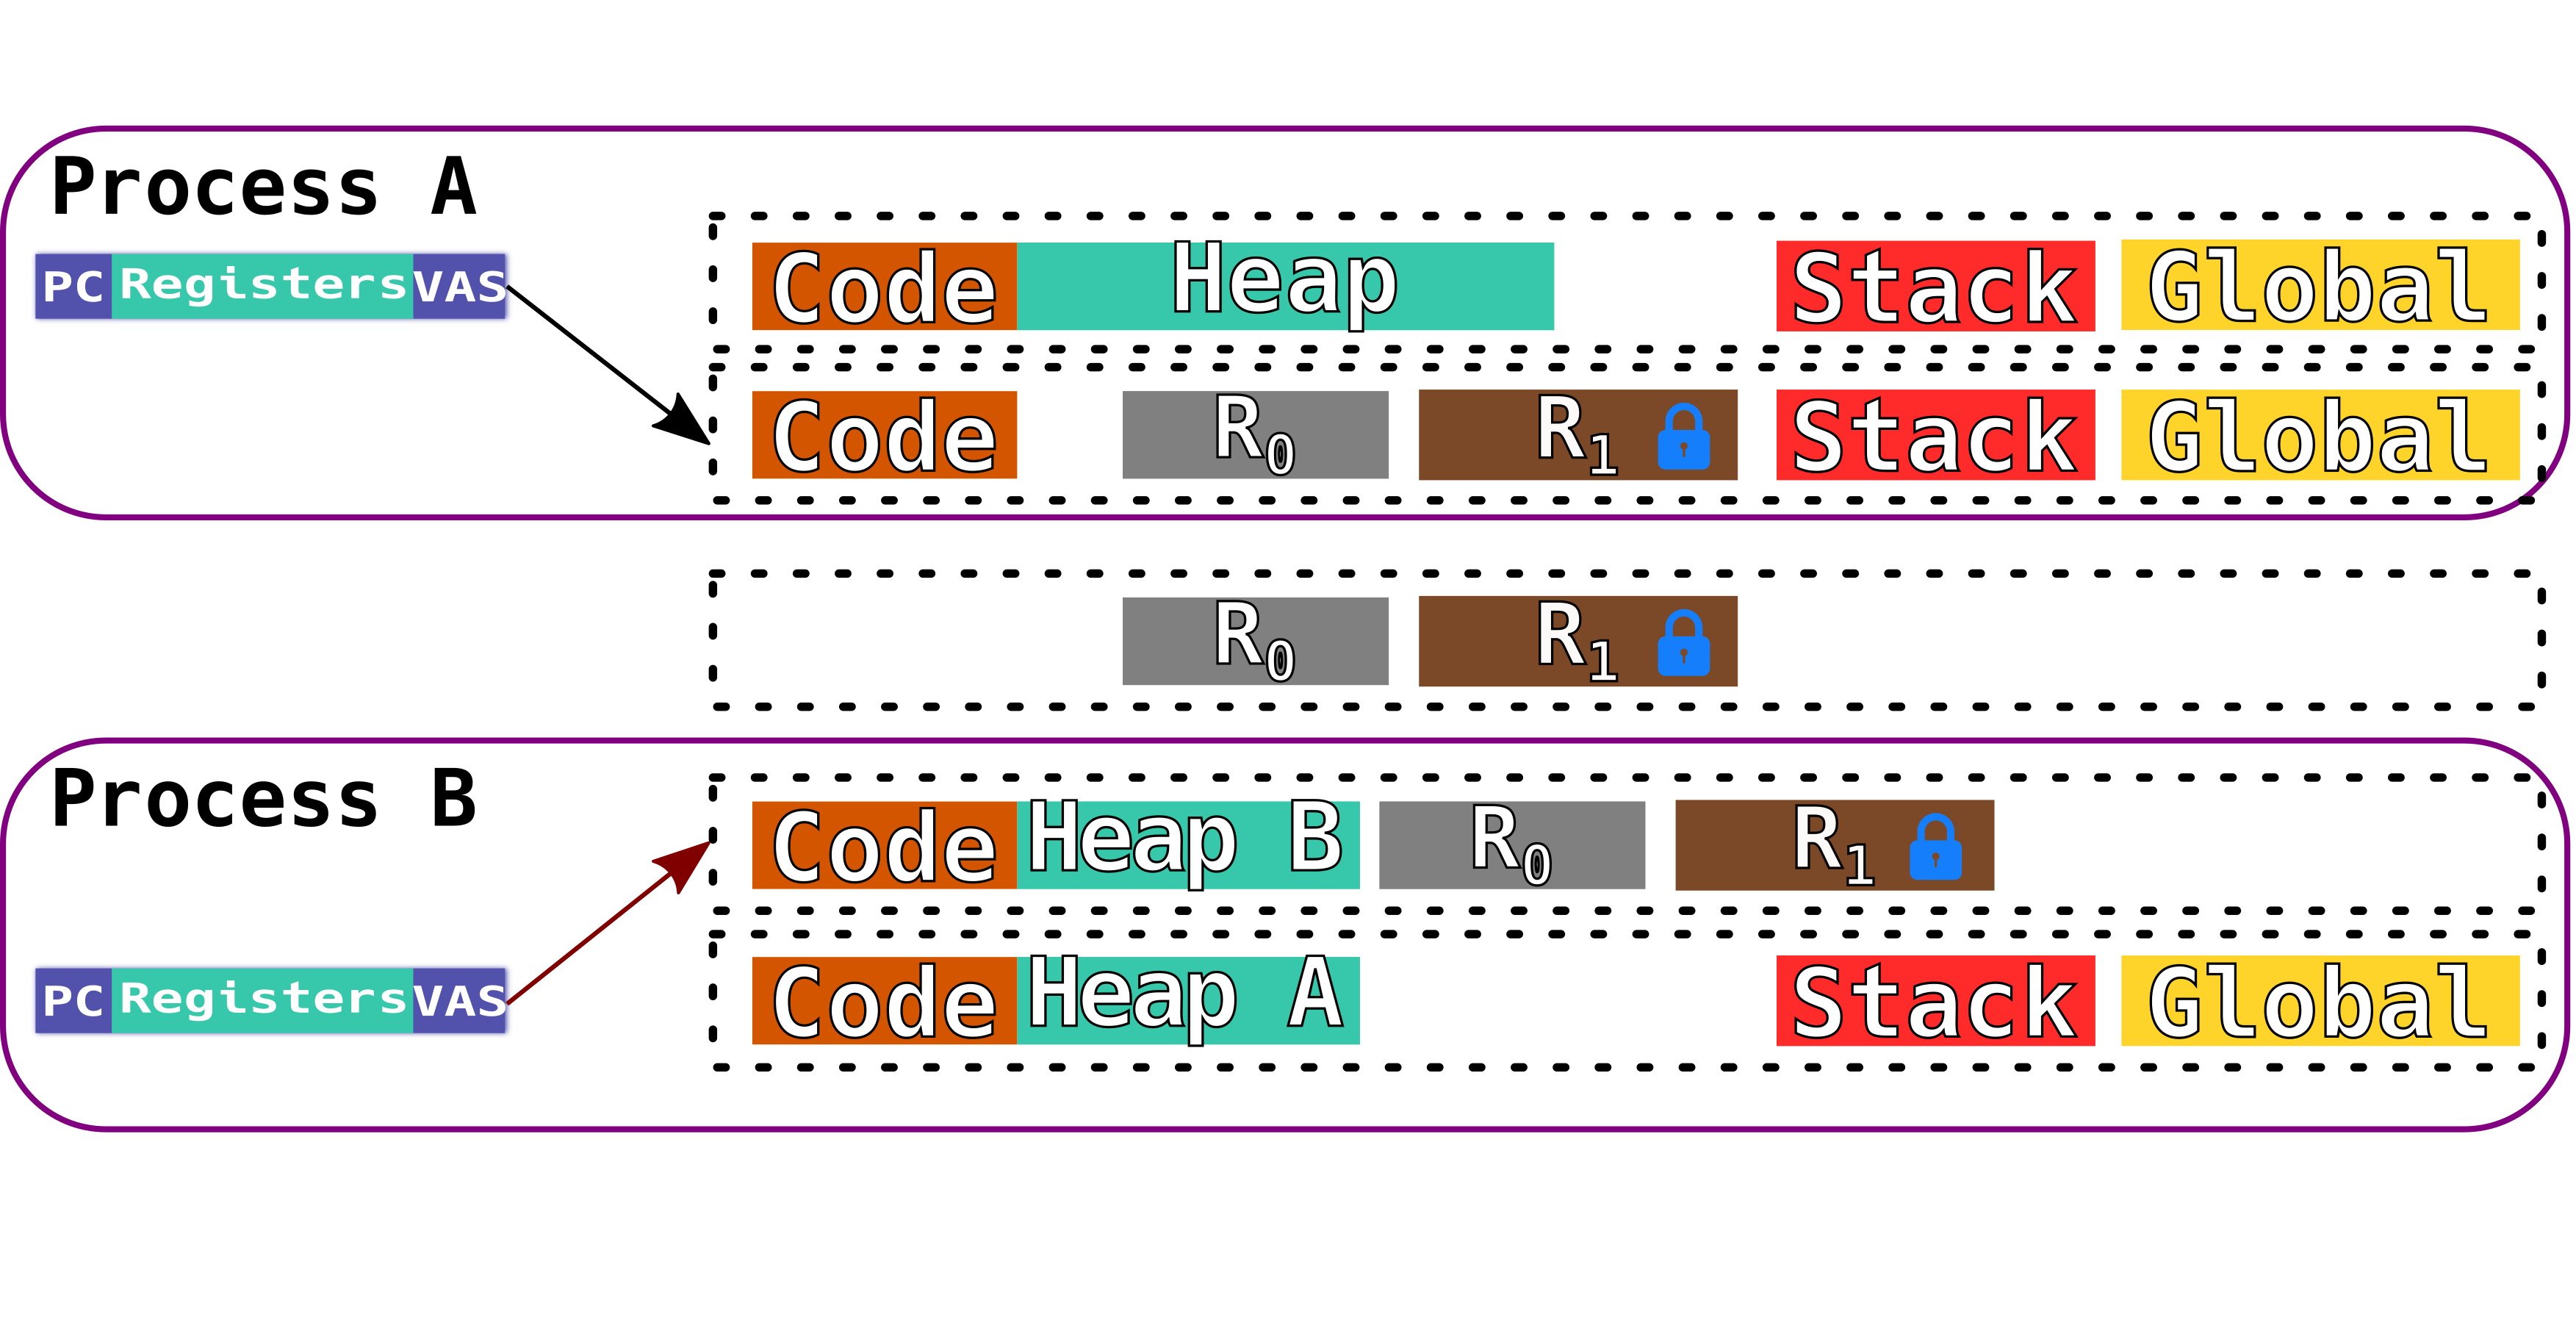
\includegraphics[width=1\textwidth, keepaspectratio=true]{images/spacejmp_example_o.png}
  \end{figure}
\end{frame}

%-------------------------------------------------------
% Implementation
%-------------------------------------------------------
\section{Implementation and Conclusion}
\begin{frame}{Implementation}{Implementation and Conclusion}
%-------------------------------------------------------
  \begin{columns}[T]
    \begin{column}{.5\textwidth}
      \begin{figure}[ht]
        \centering
        
\includegraphics[width=0.6\textwidth, keepaspectratio=true]{images/DragonFlyBSD.png}
      \end{figure}
      \url{http://www.barrelfish.org/}
    \end{column}

    \pause

    \hfill
    \begin{column}{.5\textwidth}
      \begin{figure}[ht]
        \centering
        
\includegraphics[width=0.5\textwidth, keepaspectratio=true]{images/barrelfish.png}
      \end{figure}
      \url{https://www.dragonflybsd.org/}
    \end{column}
  \end{columns}
\end{frame}

%-------------------------------------------------------
% End
%-------------------------------------------------------
{\1
\begin{frame}[plain,noframenumbering]
  \finalpage{New memory management \\ Rodrigo Siqueira \\ siqueira@kuniri.org}

\end{frame}}

\end{document}
